\documentclass[11pt]{article}
\usepackage[a4paper,margin=1in]{geometry}
\usepackage{graphicx}
\usepackage{booktabs}
\usepackage{amsmath,amssymb}
\usepackage[expansion=false]{microtype}
\usepackage[hidelinks]{hyperref}
\usepackage{caption}
\usepackage{titlesec}
\usepackage{float}
\usepackage{xcolor}
\captionsetup{font=small,labelfont=bf,skip=6pt}
\titleformat{\section}{\normalfont\Large\bfseries}{\thesection}{0.6em}{}
\titleformat{\subsection}{\normalfont\large\bfseries}{\thesubsection}{0.6em}{}
\titlespacing*{\section}{0pt}{14pt}{6pt}
\setlength{\parskip}{0.4em}
\setlength{\parindent}{0pt}

\newcommand{\eps}{\varepsilon}
% --- review aids (REMOVE before submission) -------------------------------
% \needsinfo{...}  inline red flag: a claim that needs YOUR data/confirmation.
% \reviewnote{...} margin/inline note explaining a change or a check to run.
\definecolor{nired}{rgb}{0.78,0.05,0.05}
\definecolor{rnblue}{rgb}{0.05,0.30,0.65}
\newcommand{\needsinfo}[1]{\textcolor{nired}{\textbf{[NEEDS INFO: #1]}}}
\newcommand{\reviewnote}[1]{\textcolor{rnblue}{\small[\,note: #1\,]}}

\begin{document}

\begin{center}
{\LARGE\bfseries Memory-, Latency-, and Energy-Aware Allocation of\\[2pt]
Quantized Small Language Models on a Single 8\,GB GPU\par}
\vspace{6pt}
{\large A measured, coupling-aware mixed-integer optimization for an\\
on-device multi-agent legal-assistant pipeline\par}
\vspace{8pt}
{\normalsize (Author names withheld for review)}\\
\vspace{2pt}
{\small Target hardware: NVIDIA RTX~4070 Laptop GPU (8\,GB) \quad$\bullet$\quad Case study: an on-device legal assistant}
\end{center}

\vspace{4pt}
\hrule
\vspace{8pt}

\begin{abstract}
\noindent
Deploying a multi-agent language-model pipeline on a single consumer GPU is
constrained by a fixed memory budget and by the latency and energy cost of
generation. We make three contributions, all grounded entirely in on-device
measurement. \emph{First}, we characterize the performance of $75$ quantized
small-language-model (SLM) configurations---$10$ open-weight models
($0.36$--$7.2$\,B parameters) at three \texttt{llama.cpp} K-quantization levels
and three context lengths---measured on one NVIDIA RTX~4070 Laptop GPU. We
report time-to-first-token, decode throughput, peak VRAM, and energy per token,
and we distil them into the precision, context, and scale cost curves that
govern deployment. \emph{Second}, we pose and solve
a mixed-integer linear program (MILP) that, using only these measurements,
assigns a configuration to each of the pipeline's three generation roles so as to
maximize distinct-model capacity subject to a load-once memory budget and a
serial system-latency budget $\eps$, parametric in the number $k$ of activated
specialists. The frontier is memory-bound at ${\approx}11.9$\,B and shifts rightward
with $k$. We report a deliberately strict
baseline: for this (sortable) parameter objective a greedy heuristic matches the
MILP on $92\%$ of points, so optimization adds little---and we say so. Its value
appears once the objective is not sortable: with heterogeneous specialists
(distinct legal domains, per-domain model affinities) the MILP beats greedy on
$92\%$ of points and on all points when enough specialists are active. Finally,
we report the measured-quality campaign across all three roles: quality is
\emph{non-monotone} in parameter count for the specialists---the best model is
Llama-3.2-1B, beating Mistral-7B at $6\times$ fewer parameters---so the
capacity-maximizing allocation is sub-optimal in quality at every latency budget;
conversely, routing F1 (dispatcher) and synthesis quality both \emph{rise} with
model size. The three roles thus prefer opposite ends of the model-size spectrum.
Acting on this, we build a \emph{quality-aware} allocator---the same MILP with
measured quality replacing the proxy objective---and trace the measured
quality--latency frontier. Given only measured quality it independently recovers
the three-regime structure (large dispatcher, small specialist, large
synthesiser), beats both fixed-model policies, and at matched latency dominates
the parameter-proxy allocator at every budget (mean quality gap $0.13$): the
parameter proxy and a measured-quality objective induce materially different
optima. Finally, we model the router--specialist \emph{coupling} (a specialist is
wasted if the router misroutes) as a bilinear term, linearize it exactly with
McCormick envelopes, and solve it on measured data: the gated optimum dominates
the coupling-blind additive optimum at $42$ of $44$ budgets and selects a small,
high-recall router that global-F1-based selection misses. Finally, we ask which of
these modelling choices are load-bearing: a single-family ablation shows that
\emph{both} the non-monotone specialist regime and the value of modelling
router--specialist coupling are cross-family phenomena---each collapses within a
single dense family and re-appears only across families---whereas the
small-specialist optimum is robust to the serial-versus-batched execution
model. The diversity of the candidate pool, not the latency accounting, is what the
conclusions depend on. Throughout,
``capacity'' is a parameter-count \emph{proxy}, and the heterogeneous affinities of
the optimization section are \emph{synthetic} and labelled as such. \emph{Third},
holding the static allocation fixed, we add a dynamic per-query layer that selects
which specialists to activate from a calibrated, LLM-free retrieval gate adding no
model to the memory budget: on a held-out test set of $64$ queries it raises routing
$F_1$ from $0.33$ to $0.50$ and cuts latency $9$--$35\%$ (concurrent vs.\
sequential) with a gain independent of the underlying allocation, while abstaining on
out-of-scope queries; and a single-objective concurrent-batch MILP confirms batched
serving dominates sequential serving in quality and feasibility. All data, the MILP,
the baselines, and the plotting code are released.
\end{abstract}

\vspace{4pt}

\section{Introduction}
The practical bottleneck for running language models on laptop-class hardware is
memory, not arithmetic: a model and its key--value (KV) cache must fit in a fixed
VRAM budget, often $8$\,GB or less. A \emph{multi-agent} pipeline compounds this,
because several specialised agents must co-reside and cooperate on every query.
The motivating application here is an on-device assistant for a confidentiality-
sensitive domain (legal question answering), composed of a routing
\emph{dispatcher}, nine domain \emph{specialists}, and a \emph{synthesiser} that
produces the final answer---all of which must share one GPU.

\paragraph{Three questions, one thread.} This paper is organized around three
questions that build on one another, and we use them as a thread through the
results:
\begin{description}\itemsep2pt
\item[\textbf{Q1 (Cost).}] \emph{Which configurations are feasible, and what do
they cost?} We measure all $75$ quantized configurations on the GPU
(§\ref{sec:method}--\ref{sec:perf}) and pose an allocation MILP that maximizes a
transparent capability \emph{proxy}---distinct-model parameter count---under the
memory and latency budgets (§\ref{sec:milp}--\ref{sec:opt}). The honest finding: a
greedy sort matches the MILP on $92\%$ of points, so for a sortable proxy the
optimization barely earns its keep.
\item[\textbf{Q2 (Capability).}] \emph{Is the proxy the right objective?} We run a
measured-quality campaign across all three roles (§\ref{sec:quality}) and
re-optimize on measured quality (§\ref{sec:qmilp}). The answer is no: quality is
non-monotone in size, the roles follow three distinct scaling laws, and the
quality-aware optimum is a \emph{mixed} allocation that beats the proxy at every
budget.
\item[\textbf{Q3 (Coupling).}] \emph{Do the roles interact?} A specialist is wasted
if the dispatcher misroutes it, so we model the router--specialist coupling as a
\emph{bilinear} term, solve it exactly on measured data (§\ref{sec:bilinear}), and
sweep the coupling strength to show \emph{when} optimization is worth it. The gated
optimum differs from the additive one, and the value of optimization grows with
coupling.
\item[\textbf{Q4 (Generality).}] \emph{Which modelling choices are load-bearing?}
The results rest on two deliberate choices: a \emph{heterogeneous} pool spanning
six model families, and a \emph{serial} latency chain. We test both---we
restrict the pool to a single dense family (§\ref{sec:family-ablation}) and we
re-solve the quality-aware allocator under an exact \emph{batched} execution
model (§\ref{sec:batching})---and find an asymmetry: the non-monotone
specialist regime collapses within one family, whereas the small-specialist optimum
is robust to the execution model. Heterogeneity is load-bearing for the
\emph{finding}; the latency model is not load-bearing for the \emph{optimum}.
\item[\textbf{Q5 (Adaptivity).}] \emph{Once the substrate is allocated, can the
pipeline adapt per query?} The allocation above is \emph{static}: every query pays
for the same activated specialists. We add a \emph{dynamic} layer
(§\ref{sec:dynamic}) that, holding the allocation fixed, decides per query
\emph{which} specialist domains to run---making the activation count $k(q)$
endogenous---from a calibrated, LLM-free retrieval gate that loads no model and so
adds nothing to the memory budget. On held-out queries it raises routing $F_1$ from
$0.33$ to $0.50$ and cuts latency $9$--$35\%$ (concurrent vs.\ sequential) with a
gain \emph{independent} of the underlying allocation, and a single-objective
concurrent-batch MILP confirms batched serving dominates sequential serving in
quality and feasibility.
\end{description}
The arc is therefore: cost says ``optimization is optional,'' capability says ``the
objective was wrong,'' coupling says ``the roles do not decouple, so a
per-role exact allocator is what the problem needs,'' generality says ``and the
result depends on pool diversity, not on the execution accounting,'' and adaptivity
says ``and the allocated substrate can be made query-adaptive at no extra memory
cost.'' Throughout we separate
\emph{cost} (measured) from \emph{capability} (measured quality), and we are
explicit about what each step establishes.

\section{Related Work}
\label{sec:related}
Our problem sits at the intersection of five lines of work: model cascades and
cost-aware serving, query-level routing, multi-agent LLM pipelines, reference-free
RAG evaluation, and on-device quantized inference. We review each and then state
precisely how MAMAP-Edge differs.

\paragraph{Model cascades and cost-aware serving.}
Cascades route easy queries to small models and defer hard ones to large models,
trading latency for quality~\cite{cascadetrain,semanticcascade}. The closest work
to ours is \textbf{Cascadia}~\cite{cascadia}, which also uses a mixed-integer
linear program for LLM serving: at its inner level it selects resource allocations
and parallelism strategies, while an outer level co-optimizes the routing policy.
Chen et al.~\cite{cascaderouting} unify routing and cascading into a single
framework, prove optimality conditions, and---most relevant to us---identify
\emph{when} each paradigm helps, showing that the quality of the per-model quality
estimator is the deciding factor. A recent survey~\cite{routingsurvey} catalogues
this fast-growing area. These systems share our concern with the cost--quality
frontier and our use of integer programming, but they all operate \emph{per query}
on a cascade or routing decision over interchangeable general-purpose models. We
instead make a \emph{static} allocation of \emph{fixed} models to \emph{fixed
heterogeneous roles} in a parallel multi-agent pipeline, under a hard single-GPU
memory budget---a different decision variable and a different constraint regime.

\paragraph{Query-level routing.}
\textbf{RouteLLM}~\cite{routellm} learns, from human-preference data, to route each
query to a strong or weak model, cutting cost by more than $2\times$ without quality
loss and transferring across model pairs. Routing answers ``which single model for
\emph{this} query''; our dispatcher does route queries to specialist domains, but
the paper's optimization question is orthogonal: ``which model should permanently
\emph{serve} each role,'' given that all roles must co-reside on one GPU. Routing
and our allocation are complementary---a deployed MAMAP-Edge pipeline still routes
queries at run time; we optimize the fixed substrate it routes over.

\paragraph{Multi-agent LLM pipelines.}
Multi-agent systems decompose a task across collaborating LLMs. \textbf{Mixture-of-Agents}~\cite{moa}
layers ``proposer'' models whose outputs an ``aggregator'' synthesizes---structurally
identical to our specialists-plus-synthesiser stage---and shows open models can
collaborate to match a larger one. Surveys~\cite{masurvey} taxonomize collaboration
structures (centralized, peer-to-peer), and recent work questions when mixing
\emph{different} models actually helps. This literature studies the \emph{quality}
benefit of collaboration but almost never the \emph{deployment} question of fitting
the agents onto constrained hardware, nor the \emph{coupling} between an upstream
router's accuracy and a downstream agent's usefulness, which we model explicitly.

\paragraph{Reference-free RAG evaluation.}
\textbf{RAGAS}~\cite{ragas} introduced reference-free metrics---faithfulness,
answer relevance, and context relevance---for RAG pipelines, validated against
human judgement and now widely used. Our quality campaign adopts the RAGAS metric
family (faithfulness, answer relevancy, context precision/recall) but computes the
generation metrics with embedding similarities under an \emph{oracle-retrieval}
protocol, isolating generation quality from retrieval quality
(§\ref{sec:setting-retrieval}); we use these scores not to evaluate a single system
but as the \emph{objective} of an allocation optimizer.

\paragraph{On-device and quantized small models.}
A growing body of work studies running quantized models at the edge with
\texttt{llama.cpp}/GGUF and related runtimes~\cite{edgeslm,ondevicellm}. Notably,
\textbf{SLMQuant}~\cite{slmquant} shows that small models have \emph{different}
quantization sensitivity from large ones, so LLM-tuned recipes transfer poorly---
direct evidence that SLM behaviour must be characterized, not extrapolated, which
motivates our exhaustive $75$-configuration measurement. Unified quantization
evaluations on single models~\cite{quanteval} report per-format quality/throughput
trade-offs; we extend this from a single model to a pool of $11$ models across a
multi-role pipeline, and---crucially---tie the measured quality back into an
allocation decision.

\paragraph{What is new here.}
To our knowledge, no prior work combines these threads as we do: (i) a \emph{static,
role-aware} allocation of fixed quantized SLMs to the three generation roles of a
multi-agent pipeline, under a hard load-once memory budget and a serial latency
budget on a single consumer GPU; (ii) a \emph{measured-quality} objective across all
roles, showing that a parameter-count proxy and measured quality induce materially
different optima, and that quality is non-monotone in model size with three distinct
per-role scaling laws; and (iii) an explicit \emph{bilinear} model of
router--specialist coupling, linearized exactly and solved on measured data, with a
coupling sweep that quantifies \emph{when} optimization beats a greedy heuristic.
Cascadia~\cite{cascadia} and cascade routing~\cite{cascaderouting} are the nearest
neighbours in method (integer programming for serving), but they optimize per-query
cascade/routing over interchangeable models, whereas we optimize a fixed multi-agent
substrate with heterogeneous roles and measured, coupled per-role quality.

\section{Experimental Setting}
\label{sec:setting}
This section specifies, precisely, the system under study: its agents and their
roles, the model pool, the evaluation data and legal corpora, the inference
stack, and the quality metrics. All artifacts are released.

\subsection{Agent architecture and roles}
The application is an on-device assistant for \textbf{Italian family law},
organized as an eleven-agent pipeline with three role types
(Table~\ref{tab:agents}). A single \textbf{dispatcher} reads the incoming query
and routes it to a subset of the nine domain \textbf{specialists}; the activated
specialists answer in parallel using retrieved legal context; and a single
\textbf{synthesiser} composes the activated specialists' answers into the final
user-facing response. The dispatcher is on the critical path but generates only a
short routing decision; the specialists and the synthesiser generate full answers.
Each agent declares a minimum context length $c_{\min}$ it requires
(Table~\ref{tab:agents}), which constrains which configurations may serve it. The
per-query execution order---dispatcher, then the activated specialists run serially
on their shared instance (stage cost $k\,L_{\mathrm{spec}}$), then synthesiser---defines
the system latency chain (§\ref{sec:milp}); the batched alternative, in which the
stage cost is a single specialist generation, is reported as the opposite extreme in
§\ref{sec:batching}.

\begin{table}[H]
\centering
\caption{The eleven agents (from \texttt{agents.yaml}). The nine specialists map
one-to-one to Italian family-law domains. $c_{\min}$ is the minimum context the
agent requires.}
\label{tab:agents}
\small
\begin{tabular}{@{}llr@{}}
\toprule
Role & Agent (domain) & $c_{\min}$ \\
\midrule
dispatcher & routing / classification & $2048$ \\
\midrule
specialist & testate succession (\emph{succ.\ testamentaria}) & $4096$ \\
specialist & intestate succession (\emph{succ.\ legittima}) & $4096$ \\
specialist & consensual separation (\emph{sep.\ consensuale}) & $4096$ \\
specialist & contested separation (\emph{sep.\ contenziosa}) & $8192$ \\
specialist & assisted negotiation \& mediation & $4096$ \\
specialist & minor protection (\emph{tutela minori}) & $8192$ \\
specialist & community of property (\emph{patr.\ comunione}) & $4096$ \\
specialist & separation of property (\emph{patr.\ separazione}) & $4096$ \\
specialist & non-contentious jurisdiction (\emph{vol.\ giurisdizione}) & $4096$ \\
\midrule
synthesiser & final-answer composition & $8192$ \\
\bottomrule
\end{tabular}
\end{table}

\subsection{Model pool}
Any agent can be served by any of \textbf{10 open-weight instruction-tuned models}
spanning $0.36$--$7.2$\,B parameters (Table~\ref{tab:models}), each available in
$2$--$3$ \texttt{llama.cpp} K-quantizations and three context lengths
($2048/4096/8192$). The full grid yields \textbf{75 candidate configurations}
(model $\times$ quantization $\times$ context). The pool deliberately mixes six
dense decoder-only families (Qwen2.5, Llama-3.2, Gemma-2, Phi-3.5, SmolLM2,
Mistral).

\begin{table}[H]
\centering
\caption{The 10-model pool (from \texttt{catalog\_zoo.yaml}). Each model is built
at the listed quantizations and three contexts ($2048/4096/8192$), giving $75$
configurations in total.}
\label{tab:models}
\small
\begin{tabular}{@{}llr l@{}}
\toprule
Key & HuggingFace id & Params & Quantizations \\
\midrule
smollm2-360m & SmolLM2-360M-Instruct & $0.36$ & Q3/Q5/Q8 \\
qwen2.5-0\_5b & Qwen2.5-0.5B-Instruct & $0.5$ & Q3/Q5/Q8 \\
llama3.2-1b & Llama-3.2-1B-Instruct & $1.2$ & Q5/Q8 \\
qwen2.5-1\_5b & Qwen2.5-1.5B-Instruct & $1.5$ & Q3/Q5/Q8 \\
smollm2-1\_7b & SmolLM2-1.7B-Instruct & $1.7$ & Q3/Q5/Q8 \\
gemma2-2b & gemma-2-2b-it & $2.6$ & Q5/Q8 \\
qwen2.5-3b & Qwen2.5-3B-Instruct & $3.0$ & Q3/Q5/Q8 \\
llama3.2-3b & Llama-3.2-3B-Instruct & $3.2$ & Q5/Q8 \\
phi3.5-mini & Phi-3.5-mini-instruct & $3.8$ & Q3/Q5 \\
mistral-7b & Mistral-7B-Instruct-v0.3 & $7.2$ & Q3/Q5 \\
\bottomrule
\end{tabular}
\end{table}

\subsection{Evaluation data and legal corpora}
\textbf{Query set.} Evaluation uses \textbf{25 hand-curated Italian family-law
queries} (\texttt{calib\_clean\_with\_gold\_text.yaml}), each annotated with: the
expected specialist set (gold routing), a difficulty label
(simple/medium/complex: $5/8/12$), a risk level (low/medium/high: $8/8/9$), a
category, and a \textbf{gold answer with gold supporting authorities}---both
statute IDs/passages and case IDs/passages. Queries activate $2.68$ specialists
on average (median $2$, max $6$), so most require multi-specialist synthesis. We
note plainly that $25$ queries is a small evaluation set
(§\ref{sec:quality}, §\,Limitations).

\textbf{Retrieval corpora.} Specialists answer with retrieval-augmented generation
over two curated Italian legal corpora: a \textbf{statute corpus} of $63$ articles
(\texttt{LawCorpus\_IT}; $60$ Codice Civile, $2$ Codice di Procedura Civile, and
Art.~$5$ D.Lgs.~$28$/$2010$ on mediation), and a \textbf{case-law corpus} of $61$
items (\texttt{CaseCorpus\_IT}; $57$ court decisions identified by ECLI, $3$
mediation records, $1$ notarial act). The gold authorities annotated on each query
are drawn from these corpora, enabling the retrieval and grounding metrics below.

\subsection{Inference stack and measurement}
All models run fully GPU-offloaded via \texttt{llama.cpp} on a single
\textbf{NVIDIA RTX 4070 Laptop GPU ($8$\,GB, $\approx$$6.99$\,GB usable}) under the
Windows WDDM driver, with greedy decoding. For every configuration we measure peak
VRAM, time-to-first-token, throughput, and energy per token
(\texttt{perf\_table.parquet}; medians over repeated runs), as detailed in
§\ref{sec:method}. Latencies for an $N$-token answer are derived as
$\mathrm{TTFT}+N/\mathrm{throughput}$, with role-specific $N$ ($15$ routing tokens
for the dispatcher, $384$ for specialists and the synthesiser).

\subsection{Retrieval: corpus indexing, chunking, and FAISS}
\label{sec:setting-retrieval}
The specialists and synthesiser are retrieval-augmented. We describe the indexing
pipeline (\texttt{build\_faiss.py}, \texttt{scoring/\{corpus,embeddings,retrieval\}.py})
exactly as implemented.

\textbf{Unit of indexing (``chunking'').} The corpora are pre-segmented at the
\emph{legal-unit} level rather than by fixed-size windows: each statute article
(e.g.\ \texttt{IT\_CC\_art\_602}) and each case/mediation/notarial passage (e.g.\
\texttt{ECLI:IT:TRGO:2018:431}) is one atomic document with its own id and text.
The index is therefore built over $63$ statute units and $61$ case units
(§\ref{sec:setting}); there is no sub-article windowing or overlap, because Italian
civil-code articles are already short, self-contained legal norms and splitting
them would fragment a single rule across chunks. Each \texttt{(id, text)} pair maps
one-to-one to a vector and a manifest entry.

\textbf{Embeddings.} Documents and queries are embedded with \textbf{BAAI/bge-m3}
(multilingual, including Italian; $1024$-dimensional) via \texttt{sentence-trans\-formers}.
All vectors are \textbf{L2-normalized}, so inner product equals cosine similarity.
A dependency-free hashing embedder (also $1024$-d, unigram$+$bigram) is provided
solely to validate the pipeline offline; all reported results use bge-m3.

\textbf{FAISS index.} For each corpus we build a \textbf{\texttt{IndexFlatIP}}
(exact, brute-force inner-product) index and persist it alongside a JSON
\emph{manifest} listing the document ids in index-add order---FAISS stores only
vectors, so the manifest is what maps a hit back to its id and text. We keep two
separate indexes (statutes and case law) mirroring the gold-set split. Because the
corpora are small ($\mathcal{O}(10^2)$ vectors), an exact flat index is both
feasible and preferable to an approximate one (IVF/HNSW): retrieval latency is
negligible and recall is not sacrificed to quantization. At query time the
embedded query searches both indexes for the top-$k$, results are merged,
deduplicated by id, and the top-$k$ passage texts are returned as RAG context (the
live retriever uses $k{=}5$).

\textbf{Oracle-retrieval evaluation (important).} For the quality campaign in this
paper, the generation metrics are computed under \emph{oracle retrieval}: each
query carries gold supporting-authority ids, and their texts are supplied directly
as the context (\texttt{CorpusStore.contexts\_for}). This isolates
\emph{generation} quality from \emph{retrieval} quality---we measure how well a
model uses the correct context, not whether FAISS surfaces it. A direct consequence
is that context-precision/recall against the gold ids are trivially high by
construction and are \emph{not} informative about the live retriever in these runs;
the separate retriever diagnostic (§\ref{sec:quality-retriever}) reports the live
FAISS retrieval quality. We state this explicitly because it bounds what the quality
numbers do and do not establish.

\subsection{Quality metrics}
\label{sec:setting-metrics}
Quality is scored \textbf{judge-free}: routing by set comparison, generation by
embedding similarity, with no LLM judge in the reported pipeline (a RAGAS-with-judge
path exists but is optional). All sub-scores lie in $[0,1]$. Let $\mathrm{emb}(\cdot)$
be the L2-normalized bge-m3 embedding and $\cos(u,v)=u^\top v$.

\textbf{Dispatcher --- routing F1.} Routing is multi-label set prediction. With
predicted specialist set $P$ and gold set $G$,
\begin{equation}
\mathrm{prec}=\frac{|P\cap G|}{|P|},\quad
\mathrm{rec}=\frac{|P\cap G|}{|G|},\quad
F_1=\frac{2\,\mathrm{prec}\cdot \mathrm{rec}}{\mathrm{prec}+\mathrm{rec}},
\label{eq:routingf1}
\end{equation}
and the dispatcher's quality is $Q_{\mathrm{disp}}=F_1$.

\textbf{Specialists/synthesiser --- generation metrics.} Given the produced answer
$a$, the gold answer $g$, and retrieved contexts $\{c_1,\dots,c_m\}$:
\begin{align}
\textsc{correctness} &= \max\!\big(0,\ \cos(\mathrm{emb}(a),\mathrm{emb}(g))\big),
\label{eq:corr}\\
\textsc{faithfulness} &= \max\!\big(0,\ \max_{1\le i\le m}\cos(\mathrm{emb}(a),\mathrm{emb}(c_i))\big),
\label{eq:faith}\\
\textsc{ans.\ relevancy} &= \cos\!\big(\mathrm{emb}(a),\mathrm{emb}(q)\big),
\label{eq:rel}
\end{align}
i.e.\ correctness is semantic agreement with the gold answer, faithfulness is the
answer's maximal support by any single context passage, and relevancy is
answer--question alignment. Context precision/recall are computed by id-set
comparison against the gold authorities and, under oracle retrieval
(§\ref{sec:setting-retrieval}), are reported only as diagnostics.

\textbf{Aggregate.} The scalar quality used everywhere (and as the quality-aware
MILP objective, §\ref{sec:qmilp}) is
\begin{equation}
Q=w_c\cdot \textsc{correctness}+(1-w_c)\cdot
\tfrac{1}{2}\big(\textsc{faithfulness}+\textsc{ans.\ relevancy}\big),
\quad w_c=0.5,
\label{eq:agg}
\end{equation}
with NaN sub-scores dropped and weights renormalized. \textbf{Context
precision/recall are deliberately excluded from $Q$}: they characterize the
retriever, not the candidate model, and would otherwise reward a model for the
retriever's behaviour. For the \textbf{synthesiser} we set $Q=\textsc{correctness}$
(grounding is still measured and stored), because the synthesiser's job is a
correct final answer; §\ref{sec:quality} shows this choice and the aggregate above
coincide closely in practice (correctness dominates the aggregate).

The campaign scores each (agent, configuration, query) triple and aggregates to
per-(agent, configuration) scores (\texttt{quality\_scorecard.csv}). One evaluation
convention is load-bearing and stated here: the synthesiser is scored on the
activated specialists' \emph{reference} answers (their largest-context
configuration), so its score is independent of the allocation and keeps the
optimizer linear (§\ref{sec:milp}).

\section{Measurement Methodology}
\label{sec:method}
\textbf{Configuration space.} We evaluate $10$ instruction-tuned open-weight
models spanning $0.36$--$7.2$\,B parameters (SmolLM2-360M/1.7B,
Qwen2.5-0.5B/1.5B/3B, Llama-3.2-1B/3B, Gemma-2-2B, Phi-3.5-mini, and Mistral-7B),
each in GGUF format at three
\texttt{llama.cpp} K-quantizations (Q3\_K\_M, Q5\_K\_M, Q8\_0) and three context
lengths ($2048,4096,8192$). Not every model is built at all three quantizations
(Llama-3.2, Gemma-2, Phi-3.5, and Mistral-7B omit some), so the catalogue yields
\textbf{$75$ configurations} (model $\times$ quantization $\times$ context), all of
which we measure.

\textbf{Measured quantities.} For each configuration, fully GPU-offloaded, we
record time-to-first-token (TTFT), decode throughput (tok/s), peak VRAM (NVML,
warm minus baseline), and energy per token (board power via \texttt{nvidia-smi},
minus idle, per token), each the median over repeated runs. Decoding is greedy,
with identical GGUF artefacts, so measurements are deterministic.

\textbf{Derived latency and energy.} Because end-to-end latency depends on output
length, we separate the device-fixed rate from the token count. For an answer of
$T$ tokens,
\begin{equation}
L(T)=\mathrm{TTFT}+\frac{T}{\text{throughput}},\qquad E(T)=T\cdot e_{\text{tok}},
\label{eq:derive}
\end{equation}
and we report $L,E$ at $T=384$ throughout. Equation~\eqref{eq:derive} assumes
throughput is independent of $T$, so $L$ is mildly optimistic for very long
outputs.

\textbf{Hardware and budget.} All numbers are from one NVIDIA RTX~4070 Laptop GPU
($8$\,GB GDDR6); the auto-detected usable budget at test time is
$M\approx6.99$\,GB. The device is the unit of measurement.

\section{Performance Characterization}
\label{sec:perf}
\textbf{Feasibility and throughput.} All $75$ measured configurations fit within
$M$ (Fig.~\ref{fig:heatmap}): the catalogue's quantization choices already exclude
the configurations that would not fit (notably $8$-bit variants of the largest
models), so feasibility is governed almost entirely by precision---every retained
$3$-, $5$-, and $8$-bit configuration fits the $6.99$\,GB budget. Decode throughput
falls as an approximate power law $\propto N^{-0.6}$ in parameter count $N$, from
$247$\,tok/s ($0.36$\,B) to $39$\,tok/s (the $7.2$\,B Mistral), with heavier quantization consistently slower at fixed size
(Fig.~\ref{fig:throughput}).

\begin{figure}[H]
\centering
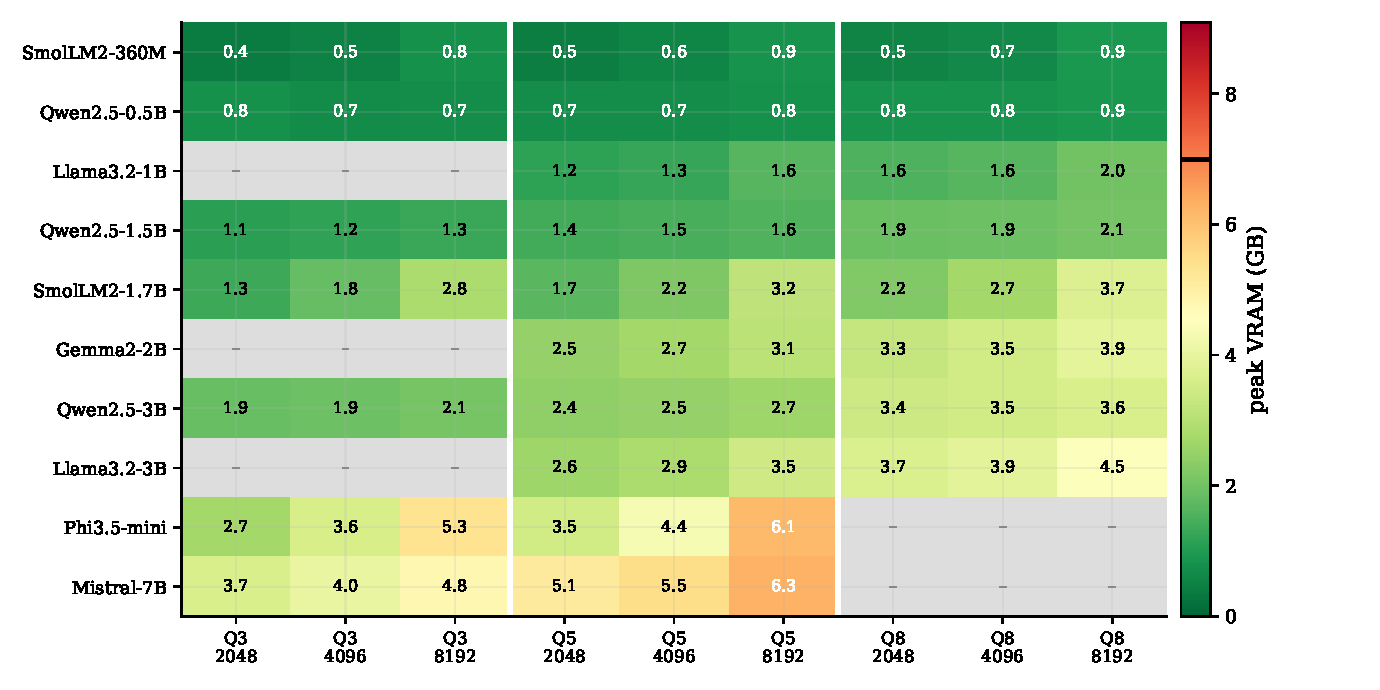
\includegraphics[width=\textwidth]{fig/heatmap.pdf}
\caption{Complete feasibility map: measured peak VRAM (GB) for all $75$
configurations ($10$ models $\times$ $3$ quantizations $\times$ $3$ contexts; grey
``--'' marks the fifteen catalogue-excluded cells: five model--quantization
combinations, at three contexts each, notably the $8$-bit builds of the two
largest models). Colour runs green (light) to red (heavy). Every released
configuration fits the $6.99$\,GB budget.}
\label{fig:heatmap}
\end{figure}

\begin{figure}[H]
\centering
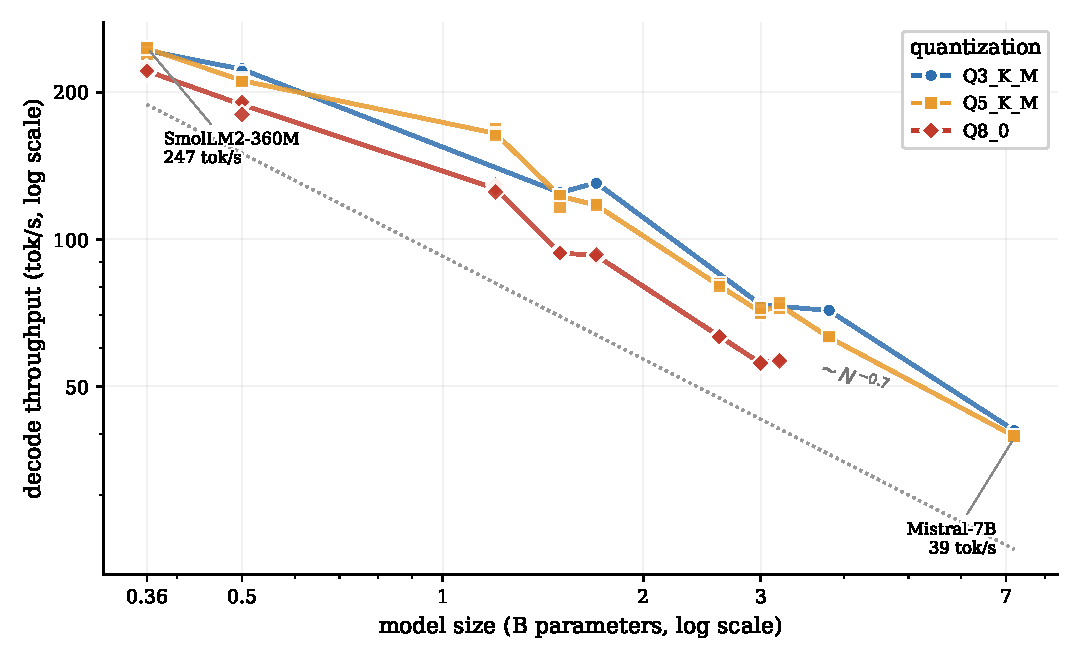
\includegraphics[width=0.82\textwidth]{fig/throughput.pdf}
\caption{Decode throughput versus model size on log--log axes (all $75$
configurations; lines are per-quantization medians). Throughput follows an
approximate power law $\propto N^{-0.6}$; heavier quantization is slower at fixed
size.}
\label{fig:throughput}
\end{figure}

\textbf{The cost of precision.} Moving from $3$- to $8$-bit weights costs, on
average at $4096$ context, $1.5\times$ in peak VRAM and $0.80\times$ in
throughput (a $20\%$ slowdown), shown per model in Fig.~\ref{fig:quant}. This
memory penalty is why the catalogue excludes the $8$-bit builds of the two largest
models (Mistral-7B, Phi-3.5) a priori; within the released grid every
configuration fits, so precision can be chosen for quality rather than forced by
memory.

\begin{figure}[H]
\centering
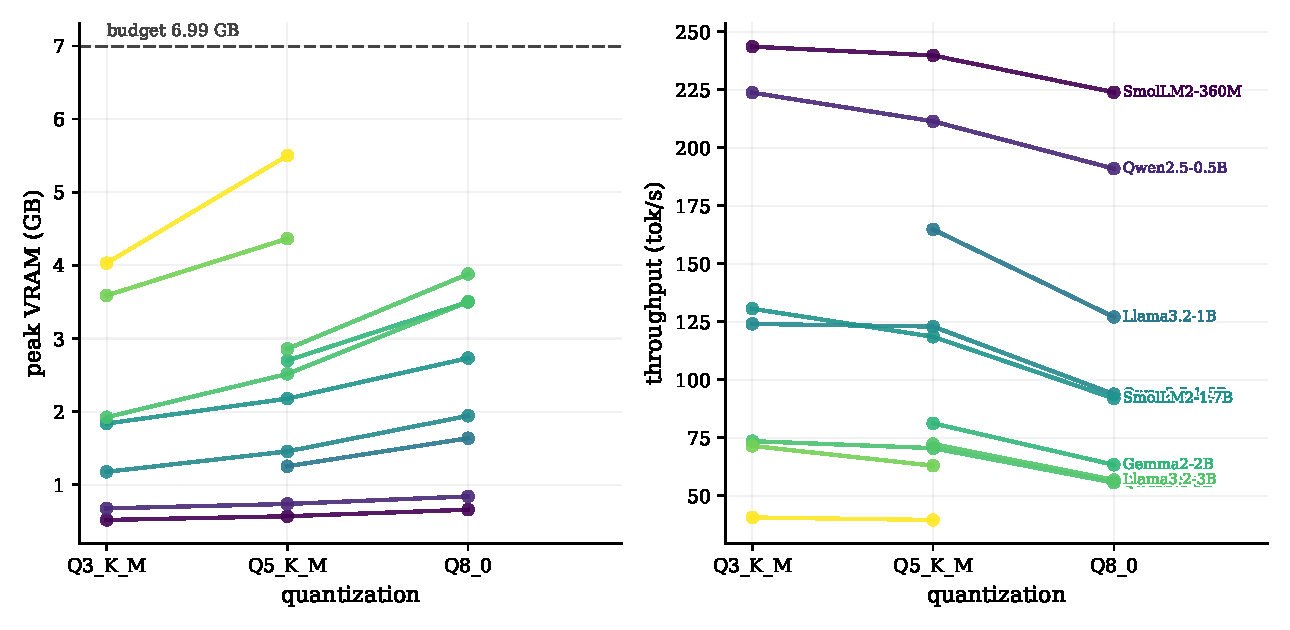
\includegraphics[width=0.92\textwidth]{fig/quant_cost.pdf}
\caption{The cost of weight precision at $4096$ context (one line per model,
colour = size). \textbf{Left:} peak VRAM rises ${\sim}1.5\times$ from Q3 to Q8;
every released configuration stays under the budget. \textbf{Right:} throughput
falls ${\sim}20\%$.}
\label{fig:quant}
\end{figure}

\textbf{The joint cost of scale.} Latency, energy, and memory rise together with
model scale, forming a coherent diagonal band in the joint cost space
(Fig.~\ref{fig:landscape}). Energy and derived latency are near-perfectly
correlated in this all-dense pool ($r{=}0.99$), so a latency budget doubles as a
tight energy budget; energy is nonetheless reported as its own measured axis
rather than folded into the latency constraint.

\begin{figure}[H]
\centering
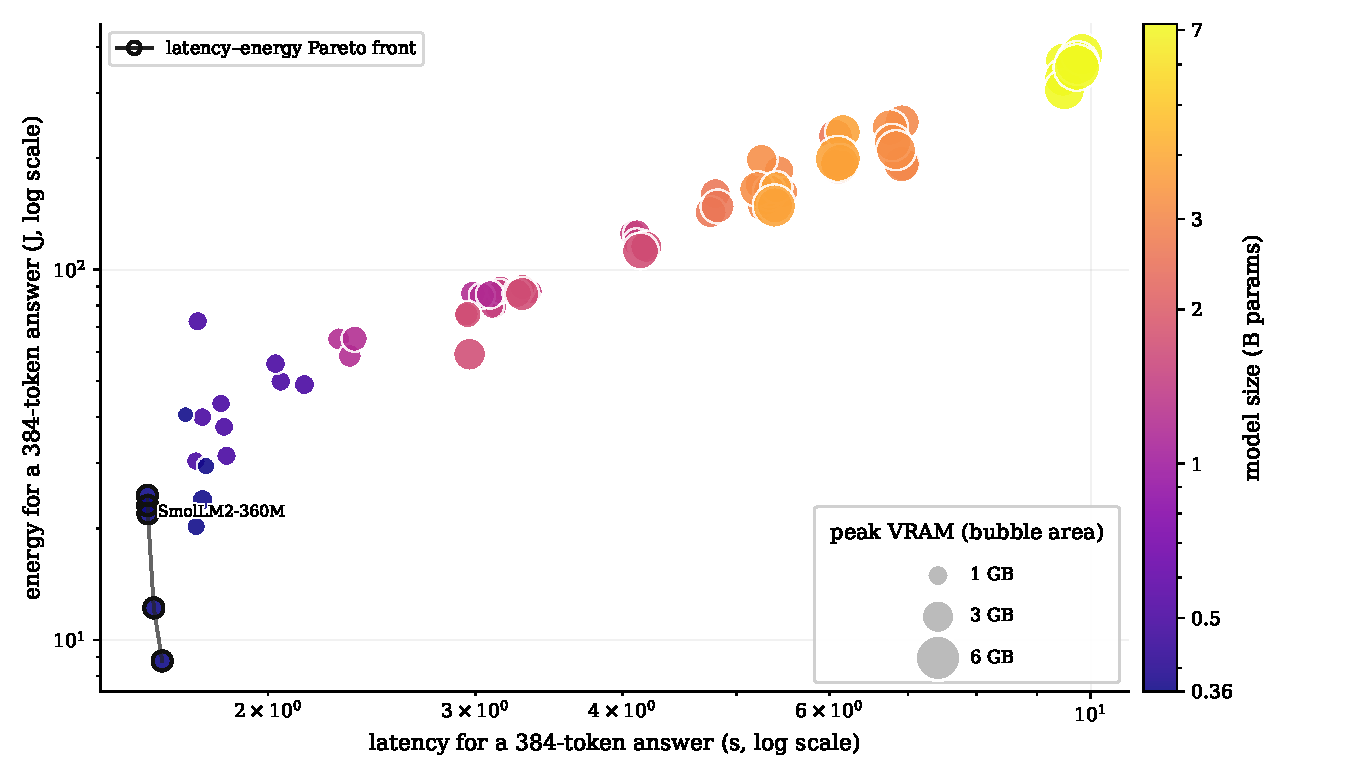
\includegraphics[width=\textwidth]{fig/cost_landscape.pdf}
\caption{The full cost landscape of all $75$ configurations, encoding
four dimensions at once: derived latency ($x$, log), derived energy ($y$, log),
peak VRAM (bubble area), and parameter scale (colour). Cost grows coherently
along the diagonal. The black curve is the latency--energy Pareto front (all its
points are the smallest model, cheapest on every axis---motivating the need for a
capability axis in Section~\ref{sec:opt}).}
\label{fig:landscape}
\end{figure}

\textbf{Cost by model family.} Grouping by family confirms the regularity the
optimizer relies on: \emph{within} a family, latency and energy scale smoothly
and predictably with size (Fig.~\ref{fig:family}); \emph{across} families at
equal size the differences are modest in this all-dense pool (at ${\approx}3$\,B,
Gemma-2 answers in $4.8$\,s against $5.3$\,s for Llama-3.2-3B and $5.5$\,s for
Qwen2.5-3B). This within-family smoothness is the structure the single-family
ablation of §\ref{sec:family-ablation} later exploits.

\begin{figure}[H]
\centering
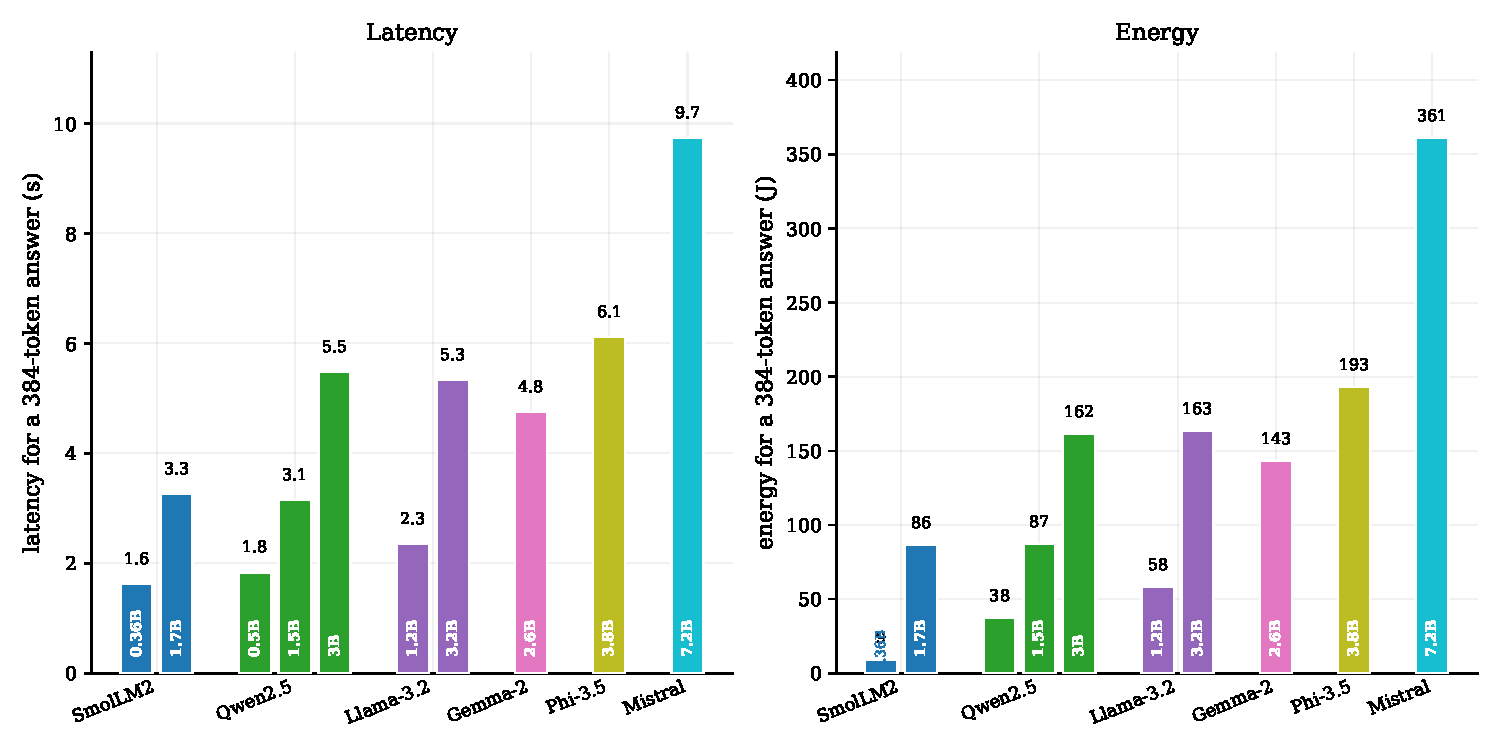
\includegraphics[width=\textwidth]{fig/family_cost.pdf}
\caption{Cost by model family (Q5\_K\_M, $4096$ context); bars grouped by family,
the parameter count printed vertically inside each bar. \textbf{Left (latency)}
and \textbf{right (energy)}: both costs grow smoothly with size within every
family.}
\label{fig:family}
\end{figure}

\textbf{How the metrics relate.} Figure~\ref{fig:corr} summarises the pairwise
Pearson correlations across all $75$ configurations. Three patterns stand out and
recur throughout the paper. Parameter count is strongly tied to peak VRAM
($0.85$) and inversely to throughput ($-0.80$), and in this all-dense pool it
predicts derived latency almost perfectly ($0.96$): bigger models are larger in
memory and slower, with no architectural exceptions. Energy per token and derived
latency are near-perfectly correlated ($0.99$), and both track parameter count
($0.95$/$0.96$)---the empirical basis for treating a latency budget as an
approximate energy budget. TTFT is the loosest axis ($|r|$ between $0.51$ and
$0.75$): it is dominated by fixed prefill overhead, though it is not independent
of scale.

\begin{figure}[H]
\centering
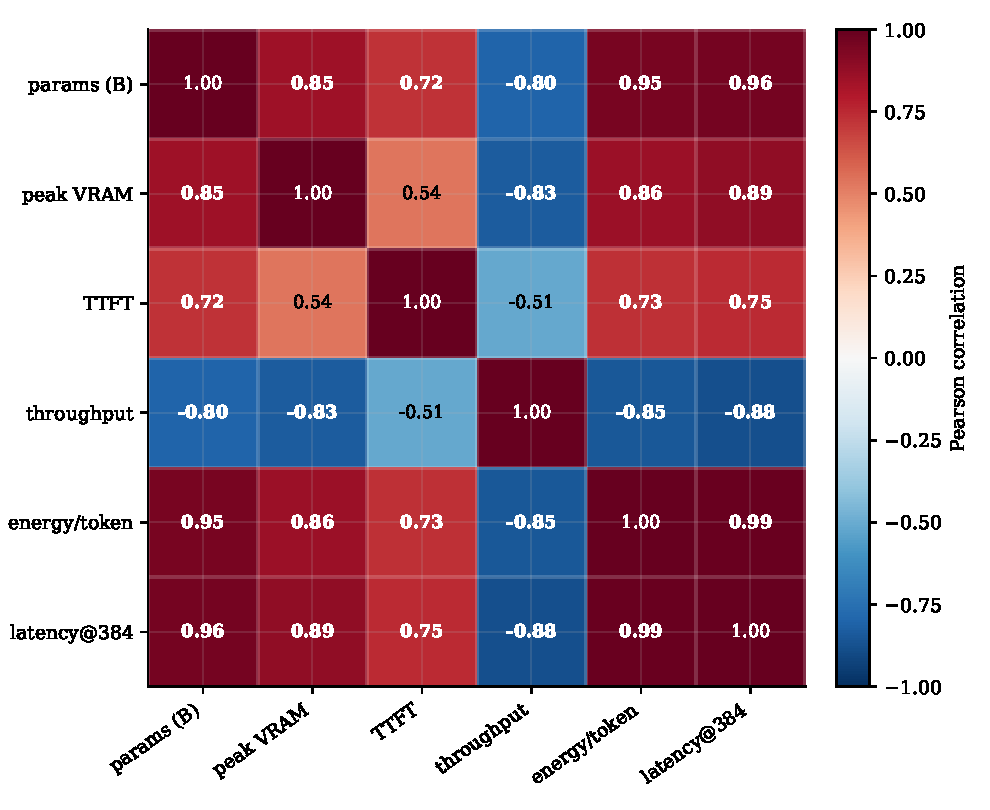
\includegraphics[width=0.72\textwidth]{fig/corr_heatmap.pdf}
\caption{Pearson correlation between the measured performance metrics (and
parameter count) across all $75$ configurations. Red is positive, blue negative.
Note the tight size/VRAM/throughput/latency couplings and the near-perfect
energy--latency correlation ($0.99$); TTFT is the loosest axis.}
\label{fig:corr}
\end{figure}

\section{The Allocation Model}
\label{sec:milp}

\subsection{The problem in plain terms}
The measurements above tell us what each configuration \emph{costs}. We now use
them to make a decision: \emph{which model should each of the eleven agents run?}
The agents are not interchangeable. One \emph{dispatcher} reads the query and
decides which specialists to invoke; nine \emph{specialists} each answer from
their own domain; one \emph{synthesiser} composes the specialists' outputs into
the final reply. Every agent needs a model resident in VRAM, and all of them
share a single $8$\,GB GPU. The allocation must therefore respect two hard
limits---a \emph{memory} budget (everything loaded must fit) and a \emph{latency}
budget (the end-to-end response must not be too slow)---while making the pipeline
as capable as possible.

\subsection{The key subtlety: how latency adds up}
\label{sec:latency-subtlety}
On a single GPU the pipeline holds \emph{one} loaded instance per model, and the
agents on the critical path execute one after another. The system latency is a
\emph{sum} along that path, and---crucially---the specialists are not all on it: the
dispatcher activates only a subset per query (that is the point of routing). The
dispatcher emits a short routing decision while the specialists and the synthesiser
emit full answers. Writing $k$ for the number of activated specialists, and treating
the specialists as running on the shared instance one after another (the conservative
accounting; see below), the chain is
\begin{equation}
L_{\text{sys}}(k) \;=\; \underbrace{L_{\text{disp}}(T_{\text{r}})}_{\text{router}}
\;+\; \underbrace{k\cdot L_{\text{spec}}(T_{\text{g}})}_{k\text{ activated specialists}}
\;+\; \underbrace{L_{\text{synth}}(T_{\text{g}})}_{\text{synthesiser}},
\label{eq:chain-intuition}
\end{equation}
where $T_{\text{r}}{\approx}15$ routing tokens and $T_{\text{g}}{=}384$ answer
tokens, and $L(\cdot)$ uses the measured per-token rate of the chosen model
(Eq.~\ref{eq:derive}). Because the specialists do the same kind of work they share
one model, so the $k$ activated terms collapse to $k\cdot L_{\text{spec}}$. This is
what makes the allocation non-trivial: every distinct model on the critical path
\emph{adds} latency, while capacity wants \emph{distinct} models---a genuine tension
between the two budgets.

\emph{Why a sum, and the batched alternative.} A specialist stage cost of
$k\cdot L_{\text{spec}}$ describes the activated specialists executing serially on the
shared instance---the \emph{conservative worst case} on latency, since several
specialists sharing one loaded model cannot run truly in parallel on one GPU. We
adopt this sum~\eqref{eq:chain-intuition} as the primary model: it is consistent with
the load-once memory accounting, and any deployment that instead \emph{batches} the
shared specialists into a single forward pass can only \emph{reduce} the specialist
term. We test that opposite extreme---an exact \emph{batched} (concurrent-stage)
model in which the stage cost is a single specialist generation $\max_{s\in\mathcal{A}}
L_{\text{spec}}$, the \texttt{worst\_case} latency mode of the released solver---in
§\ref{sec:batching}, and find the optimal allocation unchanged across the whole range
from serial to batched over the realistic budget. Since which specialists fire is
query-dependent, we do not fix $k$; we trace the frontier parametrically over
$k\in\{1,3,5,9\}$ (the calibration set activates $2.68$ specialists on average,
median $2$, maximum $6$).

\subsection{What we maximize, and the honest caveat}
The pipeline has three generation roles: the dispatcher $d$, one specialist model
$s$ shared by all specialists, and the synthesiser $y$. We maximize the
pipeline's \emph{distinct-model capacity}: the summed parameter count of the
\emph{distinct} models placed on these three slots, each model counted
\emph{once} even if two slots share it. This is the corrected objective: an
earlier version summed parameters per agent, which counted a shared model many
times and rewarded placing one large model everywhere; counting distinct models
removes that degeneracy and forces the optimizer to trade memory for variety.

\textbf{This remains a deliberate proxy, not measured answer quality.} The model
answers ``how much distinct model can the pipeline afford at a given latency,''
not ``how good are its answers.'' We use parameter count only as a stand-in for
capability; §\ref{sec:perf} showed cost scales coherently with size in this dense
pool, but cost is not capability---§\ref{sec:quality} will show the proxy is
actively misleading for specialist quality. Substituting measured per-role quality for parameter
count---once the quality campaign completes---turns the same program into a
quality-aware allocator.

\subsection{The mixed-integer linear program}
\textbf{Sets.} Three role-slots $\mathcal{R}=\{d,s,y\}$ (dispatcher, shared
specialist, synthesiser). Candidate configurations $\mathcal{C}$, each a triple
$c=(\text{model},\text{quant},\text{context})$; let $\textsf{m}(c)$ be its model
and $\mathcal{M}$ the set of models. Configurations sharing weights (same model
and quant, differing in context) form a group $g\in\mathcal{G}$.

\textbf{Measured data.} Each $c$ has parameter count $\pi_{\textsf{m}(c)}$ (B),
peak VRAM $\mu_c$ (GB), and two derived latencies---$\ell^{\text{r}}_c$ at
$T_{\text{r}}$ tokens and $\ell^{\text{g}}_c$ at $T_{\text{g}}$ tokens
(Eq.~\ref{eq:derive}). Budgets: VRAM $M=6.99$\,GB, latency $\eps$, and the
activation count $k$.

\textbf{Decision variables.}
\begin{align}
x_{r,c}&\in\{0,1\}: && \text{role $r$ runs configuration $c$;}\\
z_{c}&\in\{0,1\}: && \text{configuration $c$ is loaded in VRAM;}\\
u_{m}&\in\{0,1\}: && \text{model $m$ is used by some role (for capacity).}
\end{align}

\textbf{Objective}---maximize distinct-model capacity:
\begin{equation}
\max\ \sum_{m\in\mathcal{M}} \pi_m\,u_{m}.
\label{eq:obj}
\end{equation}

\textbf{Constraints.} In words: (\ref{eq:assign})~each role runs one
configuration; (\ref{eq:loaduse})~a role may run a configuration only if it is
loaded; (\ref{eq:onectx})~at most one context per weight-sharing group is loaded;
(\ref{eq:mem})~loaded configurations fit in VRAM, each counted once;
(\ref{eq:caplink})~a model counts toward capacity only if some role uses it;
(\ref{eq:lat})~the serial latency chain~\eqref{eq:chain-intuition} stays
within budget.
\begin{align}
\sum_{c\in\mathcal{C}} x_{r,c} &= 1 && \forall r\in\mathcal{R}
\label{eq:assign}\\
x_{r,c} &\le z_{c} && \forall r\in\mathcal{R},\,c\in\mathcal{C}
\label{eq:loaduse}\\
\sum_{c\in g} z_{c} &\le 1 && \forall g\in\mathcal{G}
\label{eq:onectx}\\
\sum_{c\in\mathcal{C}} \mu_c\,z_{c} &\le M
\label{eq:mem}\\
u_{m} &\le \!\!\sum_{r\in\mathcal{R}}\sum_{c:\textsf{m}(c)=m}\!\! x_{r,c}
&& \forall m\in\mathcal{M}
\label{eq:caplink}\\[-1pt]
\sum_{c} \ell^{\text{r}}_c x_{d,c} + k\!\sum_{c} \ell^{\text{g}}_c x_{s,c}
+ \sum_{c} \ell^{\text{g}}_c x_{y,c} &\le \eps
\label{eq:lat}
\end{align}

\textbf{Properties.} Constraint~\eqref{eq:lat} is the serial chain of
Eq.~\eqref{eq:chain-intuition}: the specialist term $k\sum_c \ell^{\text{g}}_c
x_{s,c}$ charges the $k$ activated specialists running one after another on the
shared instance (the conservative worst case; §\ref{sec:batching} shows the optimum
is unchanged under the batched alternative). The program is linear and tiny---three
role-slots over $\sim$$30$ model--quant groups---and solves in well under a second
with CBC. It is genuinely constrained on \emph{both} axes: capacity~\eqref{eq:obj}
pushes toward three distinct models, while memory~\eqref{eq:mem} and the serial
latency~\eqref{eq:lat} push back. A \emph{quality-aware} version replaces $\pi_m$
in~\eqref{eq:obj} with measured per-role quality and gates the specialist term by
the dispatcher's routing accuracy; that gating is bilinear (a product of two
binaries) and needs McCormick linearization (§\ref{sec:bilinear}).

\section{Optimization Results}
\label{sec:opt}
\emph{This section answers Q1's second half: given the measured costs, what does the
proxy-optimal allocation look like, and is the optimization even necessary?}
We solve the MILP over a sweep of the latency budget $\eps$ for each activation
level $k\in\{1,3,5,9\}$, from the smallest feasible $\eps$ (the fastest
configuration on all three slots) upward. The result is the \textbf{system
capacity--latency frontier} (Fig.~\ref{fig:frontier}).

\begin{figure}[H]
\centering
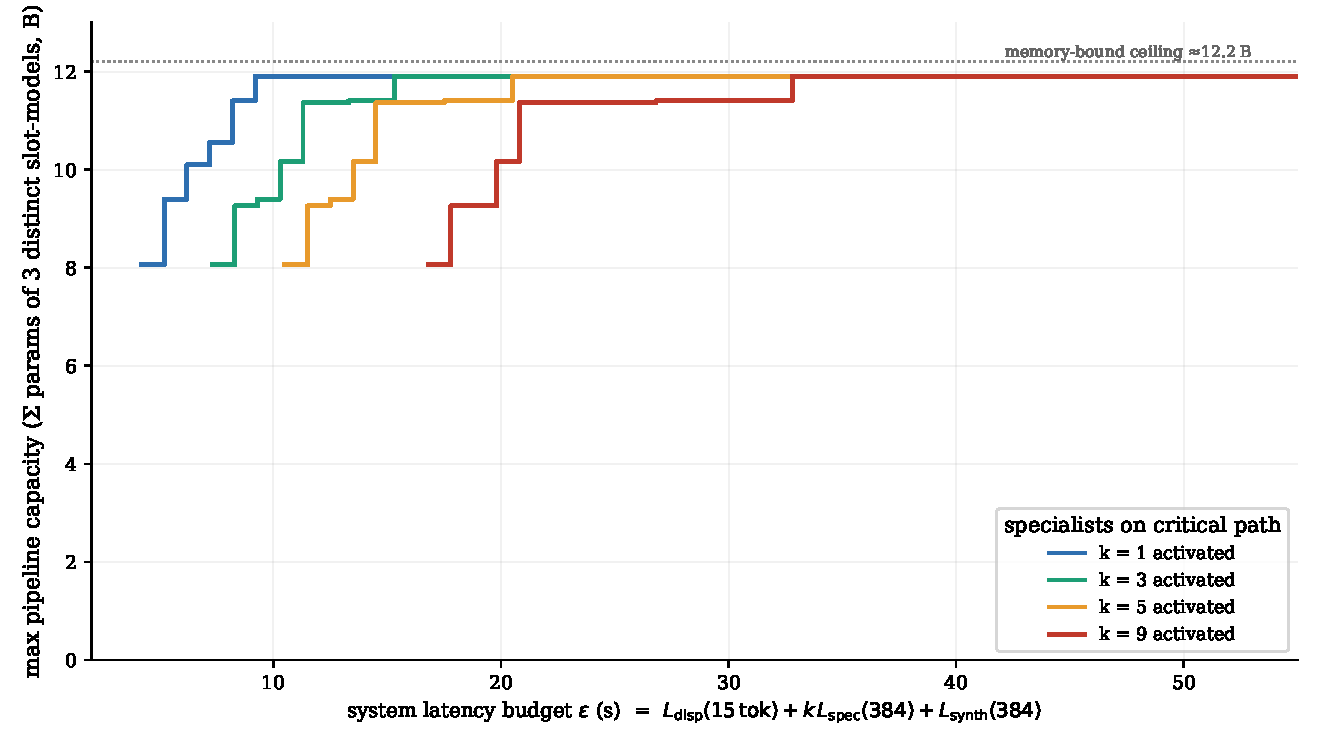
\includegraphics[width=\textwidth]{fig/syscap3_frontier.pdf}
\caption{System capacity--latency frontier under the $6.99$\,GB budget,
for $k\in\{1,3,5,9\}$ activated specialists (serial chain). Capacity (sum of the
three distinct slot-models' parameters) rises in a staircase to a memory-bound
ceiling of ${\approx}11.9$\,B. Increasing $k$ shifts the whole frontier rightward:
the same capacity costs more latency because each activated specialist adds to the
serial chain.}
\label{fig:frontier}
\end{figure}

\textbf{The ceiling is set by memory, not latency.} The frontier plateaus at
${\approx}11.9$\,B for every $k$ once $\eps$ is large enough. This ceiling is the
largest sum of three distinct models that fits in $6.99$\,GB---the optimizer
loads three models totalling $11.9$\,B and uses $6.8$\,GB at the
plateau. Memory, not the latency chain, is the binding constraint at capacity;
the latency budget only governs \emph{how soon} along $\eps$ the ceiling is
reached. (This corrects an earlier formulation in which double-counted capacity
and an inconsistent latency model produced an illusory $72$\,B figure; under
coherent accounting the realisable capacity is roughly six times smaller.)

\textbf{The cost of an active pipeline (the role of $k$).} The four curves
quantify the serial-chain penalty. With a single activated specialist
the full $11.9$\,B ceiling is reached already at $\eps{\approx}9$\,s; it requires
$\eps{\approx}15$\,s at $k{=}3$, ${\approx}21$\,s at $k{=}5$, and ${\approx}33$\,s
at $k{=}9$. Because the calibration set activates $2.68$ specialists on average,
the $k{=}3$ curve is the operationally relevant one: a full-capacity pipeline
needs a latency budget of roughly $15$\,s under realistic routing, not the
$\sim$$9$\,s a single-specialist reading would suggest. (§\ref{sec:batching} shows
that batching the shared specialists collapses this penalty---the same allocation
then reaches full capacity at a much tighter budget---without changing the optimal
allocation itself.)

\textbf{What the optimizer does (and what is \emph{not} an emergent rule).} Two
behaviours are worth noting, but neither is a deep discovery. First, the
dispatcher is consistently assigned a \emph{large} model, because with only
$T_{\text{r}}{\approx}15$ routing tokens its latency is ${\sim}0.4$\,s regardless of
size, so it is nearly free to make the dispatcher large and gain its parameters
toward capacity. This is a direct consequence of the realistic per-role token
counts, not an independent design principle. Second, the optimizer always selects
exactly three distinct models (one per slot); there is no incentive to load unused
models. Both behaviours follow mechanically from the objective and the batched
latency model.

\textbf{Frontier detail and the latency chain.} Figure~\ref{fig:annot} traces the
$k{=}3$ frontier with the specialist-tier transitions annotated, against the faint
$k\in\{1,5,9\}$ curves; Table~\ref{tab:frontier} lists its knots. The allocation
climbs by enlarging the specialist tier
(SmolLM2-360M\,$\to$\,Qwen-0.5B\,$\to$\,Llama-1B\,$\to$\,SmolLM2-1.7B) while the
dispatcher stays on a large model (cheap at $15$ routing tokens) and the
synthesiser acts as the swing slot, absorbing spare budget. Figure~\ref{fig:chain}
decomposes the critical-path latency at each knot: the dispatcher term is
negligible ($\sim$$0.4$\,s), the $k{=}3$ specialist term dominates and grows as
larger specialists are afforded, and the synthesiser fills the remaining budget;
the stacked totals track $\eps$, confirming the latency constraint binds at the
knots while memory binds at the ceiling.

\begin{figure}[H]
\centering
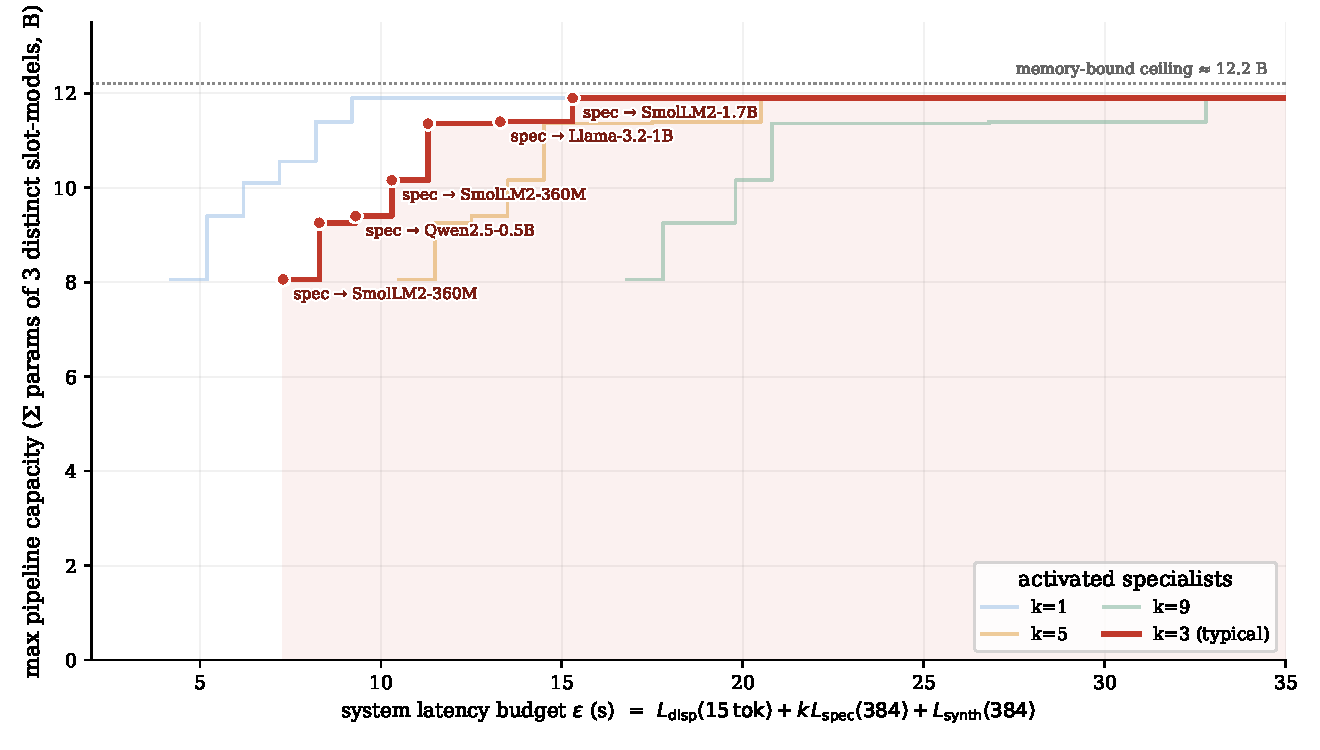
\includegraphics[width=\textwidth]{fig/frontier_annotated.pdf}
\caption{System capacity--latency frontier (serial chain) with the $k{=}3$ curve
highlighted and annotated at each specialist-tier change; faint curves are
$k\in\{1,5,9\}$. Capacity is the sum of the three distinct slot-models' parameters;
it rises in a staircase to a memory-bound ceiling of ${\approx}11.9$\,B. Larger $k$
shifts the curve rightward (more activated specialists cost more serial latency for
the same capacity).}
\label{fig:annot}
\end{figure}

\begin{table}[H]
\centering
\caption{Knots of the $k{=}3$ capacity--latency frontier (full data in
\texttt{syscap3\_frontier.csv}). ``Specialist'' is the model shared by all
specialists. Capacity counts the three distinct slot-models once each; VRAM is
the load-once total. Note the memory-bound ceiling at $11.9$\,B and the large
dispatcher (cheap at $15$ routing tokens). Listed configurations are the
\emph{canonical} optima: among objective-equal solutions the released code selects
the minimum-latency, then minimum-memory configuration, so the table is
machine-independent. $\eps$ values are under the serial $k{=}3$
chain; §\ref{sec:batching} shows the same allocations hold under batching, at tighter
budgets.}
\label{tab:frontier}
\small
\begin{tabular}{@{}rrrlll@{}}
\toprule
$\eps$ (s) & capacity (B) & VRAM (GB) & dispatcher & specialist & synthesiser \\
\midrule
7.3 & 8.1 & 5.16 & Mistral-7B & SmolLM2-360M / Q5 & Qwen2.5-0.5B \\
8.3 & 9.3 & 5.82 & Mistral-7B & SmolLM2-360M / Q5 & SmolLM2-1.7B \\
9.3 & 9.4 & 6.04 & Mistral-7B & Qwen2.5-0.5B / Q3 & SmolLM2-1.7B \\
10.3 & 10.2 & 6.81 & Mistral-7B & SmolLM2-360M / Q5 & Gemma-2-2B \\
11.3 & 11.4 & 6.82 & Mistral-7B & SmolLM2-360M / Q5 & Phi-3.5-mini \\
13.3 & 11.4 & 6.67 & Mistral-7B & Llama-3.2-1B / Q5 & Qwen2.5-3B \\
15.3 & 11.9 & 6.84 & Mistral-7B & SmolLM2-1.7B / Q3 & Qwen2.5-3B \\
\bottomrule
\end{tabular}
\end{table}

\begin{figure}[H]
\centering
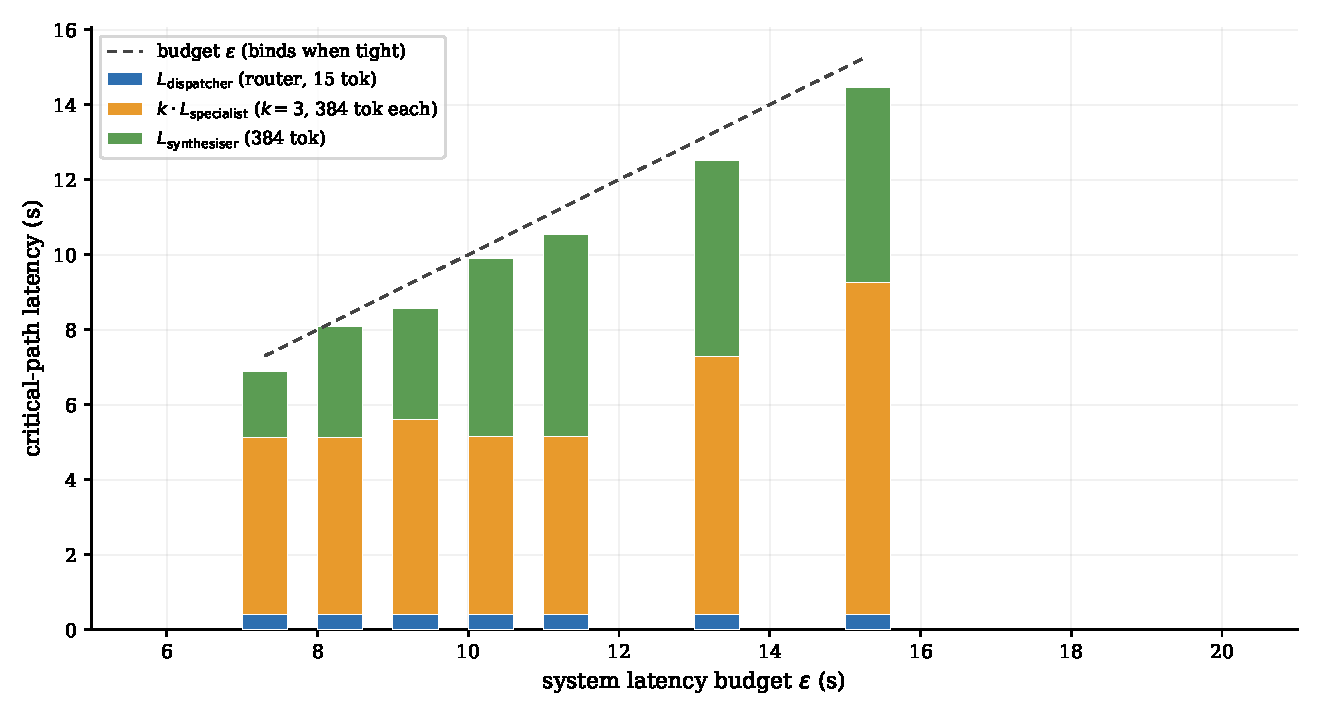
\includegraphics[width=\textwidth]{fig/chain_breakdown.pdf}
\caption{How the latency budget is spent along the serial critical path at
each $k{=}3$ knot: dispatcher (router, $15$ tokens) $+$ $k\,L_{\mathrm{spec}}$
($384$ tokens each) $+$ synthesiser ($384$ tokens). The dispatcher term is
negligible; the specialist term dominates and grows with the specialist tier; the
synthesiser absorbs the slack. The stacked totals track $\eps$, confirming the
latency constraint binds at the knots.}
\label{fig:chain}
\end{figure}

\subsection{Does the optimization beat a trivial heuristic? (performance-only)}
A strict test of whether the MILP earns its keep: we compare it against a
\emph{greedy} heuristic (independently give each slot the largest-parameter model
whose configuration keeps the chain within $\eps$ and fits memory) and a
\emph{uniform} baseline (the single largest model placed on all three slots).
Across $91$ $(\eps,k)$ points (Fig.~\ref{fig:baseline}), the honest result is
sobering: \textbf{the MILP ties the greedy heuristic at $84/91$ points
($92\%$) and strictly beats it at only $7$}, all in a narrow mid-latency band,
by $0.1$--$1.2$\,B (mean $0.56$\,B). The uniform baseline is far worse
everywhere. The reason is structural: with the parameter-count objective, the
best choice per slot is simply ``the largest model that fits the slot's latency
share,'' so the problem is \emph{sortable} and a one-line greedy reproduces it
except where the memory and latency constraints couple tightly. \textbf{On
performance-only data, the optimization adds little over a sort, and we say so.}

\begin{figure}[H]
\centering
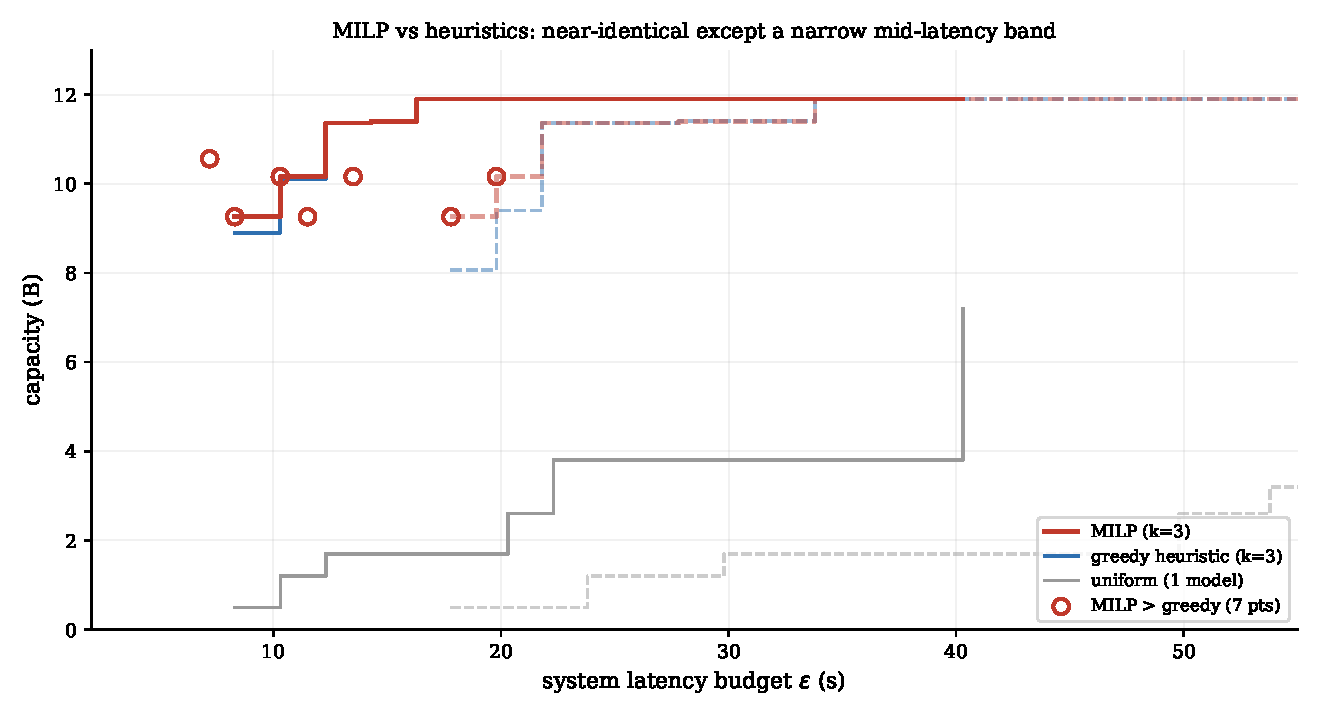
\includegraphics[width=\textwidth]{fig/baseline_cmp.pdf}
\caption{Performance-only objective (parameter capacity): MILP versus baselines
(solid $k{=}3$, dashed $k{=}9$). The MILP (red) and greedy heuristic (blue) are
nearly indistinguishable; circles mark the seven points where the MILP strictly
wins. The uniform single-model baseline (grey) is far below. When the objective
is sortable, optimization adds little over a greedy sort.}
\label{fig:baseline}
\end{figure}

\subsection{When optimization matters: heterogeneous specialists}
The greedy heuristic ties the MILP only because the parameter objective is
sortable. The realistic objective is not. The nine specialists cover
\emph{different} legal domains (testamentary vs intestate succession, consensual
vs contested separation, minor protection, family mediation, $\dots$), and a
model that is strong on one domain may be weak on another---``pick the largest''
is no longer ``pick the best.'' To quantify the effect we attach to each
$(\text{model},\text{domain})$ pair an \emph{affinity} $A_{m,\delta}\in[0,1]$ and
maximize the summed affinity of the $k$ activated specialist-domains plus the
synthesiser's quality (and a small routing-quality term for the dispatcher),
under the same memory and serial-latency constraints. The specialist slots
are now \emph{distinct} (slot $s_j$ serves domain $\delta_j$), so the MILP must
co-optimize which model serves which domain against the shared budgets---a
genuinely combinatorial problem.

\textbf{Honesty: these affinities are synthetic.} We do not yet have measured
per-domain quality (it requires the quality campaign, still running), so
$A_{m,\delta}$ here is \emph{synthetic but plausible}: each model has a latent
skill that increases with log-parameters but saturates and carries
model-specific noise, perturbed by $\pm0.12$ domain-specific deviations so that a
smaller model can top a given domain. This subsection is therefore a
\emph{demonstration of when optimization is needed}, on synthetic affinities, not
a measured result; when the quality table lands, $A_{m,\delta}$ is replaced by
measured per-domain quality and the same MILP runs unchanged.

Under this heterogeneous objective the picture inverts
(Fig.~\ref{fig:hetero}): \textbf{the MILP beats the greedy heuristic on $84/91$
points ($92\%$)}, and---tellingly---the advantage grows with the number of
activated specialists, from $25\%$ at $k{=}1$ (a near-sortable single-domain
problem, where greedy is adequate) to $94\%$ at $k{=}3$ and $100\%$ at $k{\ge}5$. The mechanism is exactly what the greedy cannot see: with
several domains competing for one shared memory budget and one serial
latency budget, the best global assignment trades a slightly worse model on one
domain for a much better one on another---a joint decision a per-slot sort cannot
make. This is the regime in which the MILP earns its keep, and it is the regime
the production system actually inhabits once answer quality, not parameter count,
is the objective.

\begin{figure}[H]
\centering
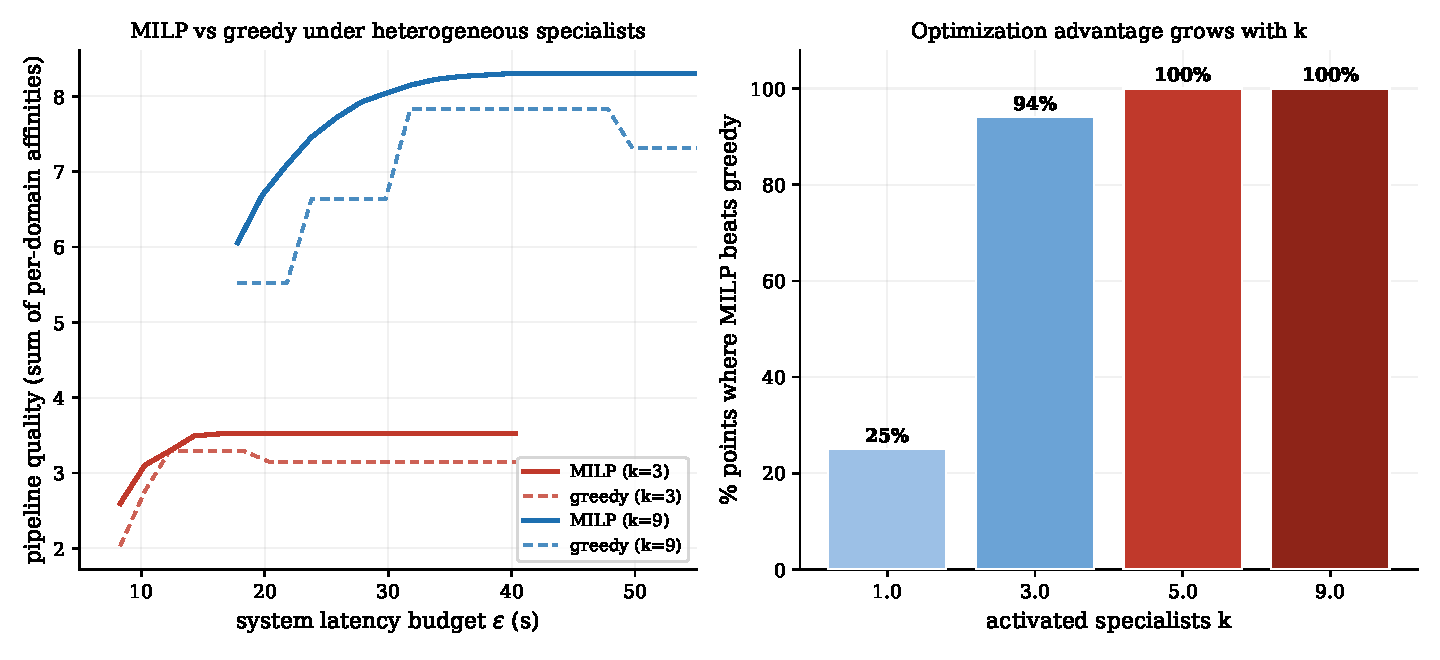
\includegraphics[width=\textwidth]{fig/baseline_hetero.pdf}
\caption{Heterogeneous-specialist objective (\emph{synthetic} per-domain
affinities, clearly labelled). \textbf{Left:} pipeline quality versus latency
budget for $k{=}3$ and $k{=}9$; the MILP (solid) dominates the greedy heuristic
(dashed) at every budget. \textbf{Right:} the fraction of points where the MILP
strictly beats greedy rises with the number of activated specialists $k$, from
$25\%$ ($k{=}1$, near-sortable) to $100\%$ ($k{\ge}5$). When the objective is not
sortable, optimization is necessary, not marginal.}
\label{fig:hetero}
\end{figure}

\subsection{Sensitivity of the frontier to measurement noise}
Lacking repeated raw runs, we test robustness by Monte-Carlo sensitivity: we
perturb every configuration's throughput and TTFT by independent lognormal noise
($\sigma{=}10\%$, a realistic laptop-GPU thermal-drift figure), recompute derived
latency, and re-solve at $k{=}3$ over $25$ draws (Fig.~\ref{fig:uncertainty}). The
frontier is stable: the $10$--$90$ percentile band is ${\pm}0.5$\,B around the
median and collapses to zero at high $\eps$, where memory binds hard and the
capacity ceiling is noise-independent. Tier transitions shift by at most a
fraction of one $\eps$ step. We label this a sensitivity analysis, not a
confidence interval from real replicates.

\begin{figure}[H]
\centering
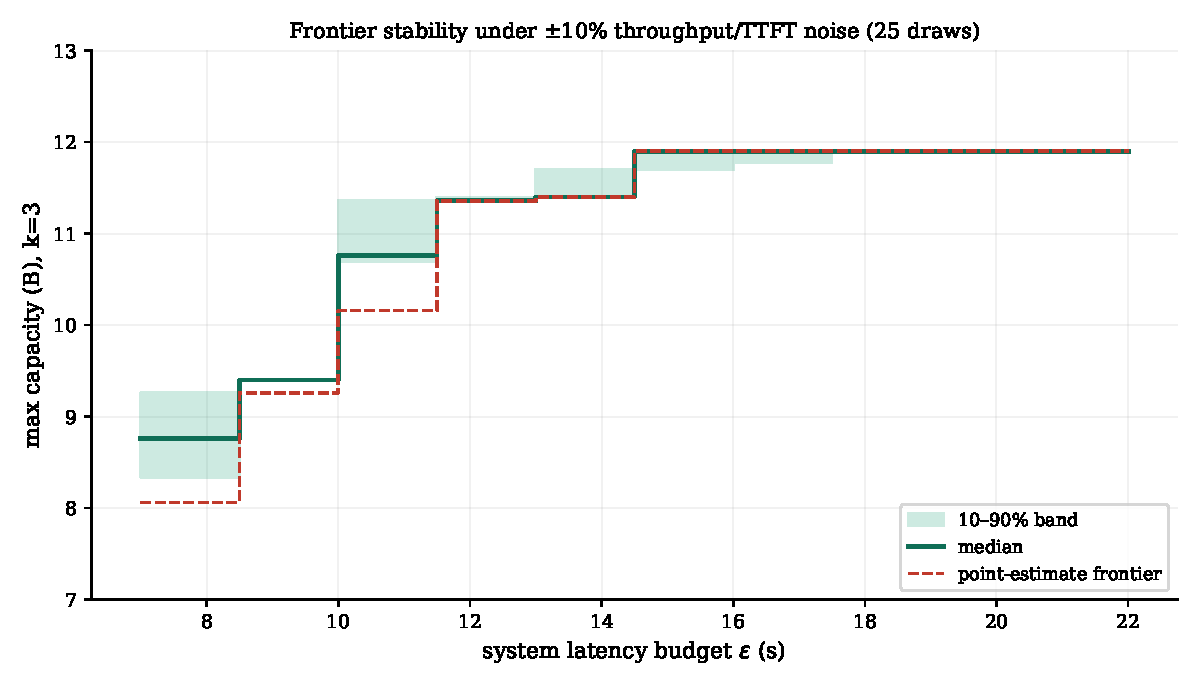
\includegraphics[width=0.86\textwidth]{fig/uncertainty.pdf}
\caption{Frontier stability at $k{=}3$ under ${\pm}10\%$ throughput/TTFT noise
($25$ draws). The $10$--$90\%$ band (shaded) is narrow and vanishes at high
$\eps$; the point-estimate frontier (dashed) sits inside it. Capacity tiers are
robust to plausible measurement variation.}
\label{fig:uncertainty}
\end{figure}

\section{Measured Quality Results (All Roles)}
\label{sec:quality}
The frontier above optimizes a parameter-count proxy. We now report the first
results of the \emph{measured}-quality campaign, which scores each agent's output
with judge-free, embedding-based metrics (routing F1 for the dispatcher; RAG
faithfulness, answer relevancy, context precision/recall, and correctness for the
specialists). These results let us answer the question the proxy cannot: \emph{is
the highest-capacity allocation actually the highest-quality one?}

\textbf{Status of the campaign.} The campaign covers all eleven agents over $75$
of $75$ configurations and $129$ query instances, with $7959$ scored
agent--query--config records: $3900$ for the dispatcher, $3439$ across the nine
specialists, and $620$ for the synthesiser. All three roles are now analyzed
below. Coverage is not yet exhaustive---a few weight-sharing groups and some
lower-frequency domains remain under-sampled---so per-domain confidence intervals
will tighten as the campaign completes, but the qualitative findings are stable.

\subsection{Quality does not track parameter count}
Across specialist configurations, measured quality correlates only weakly with
parameter count (Pearson $r{=}0.54$ at the configuration level, $0.31$ at the
per-query level) and, more importantly, the relationship is \emph{non-monotone}
(Fig.~\ref{fig:q_params}). The single best specialist model is
\textbf{Llama-3.2-1B} (mean quality $0.74$), which \emph{outscores every larger
model}, including Mistral-7B ($0.72$) at $6\times$ the parameters, and Phi-3.5.
Conversely, Qwen-0.5B is the \emph{worst} model despite not being the
smallest. Parameter count is thus an actively misleading capability proxy for the
specialist role.

\begin{figure}[H]
\centering
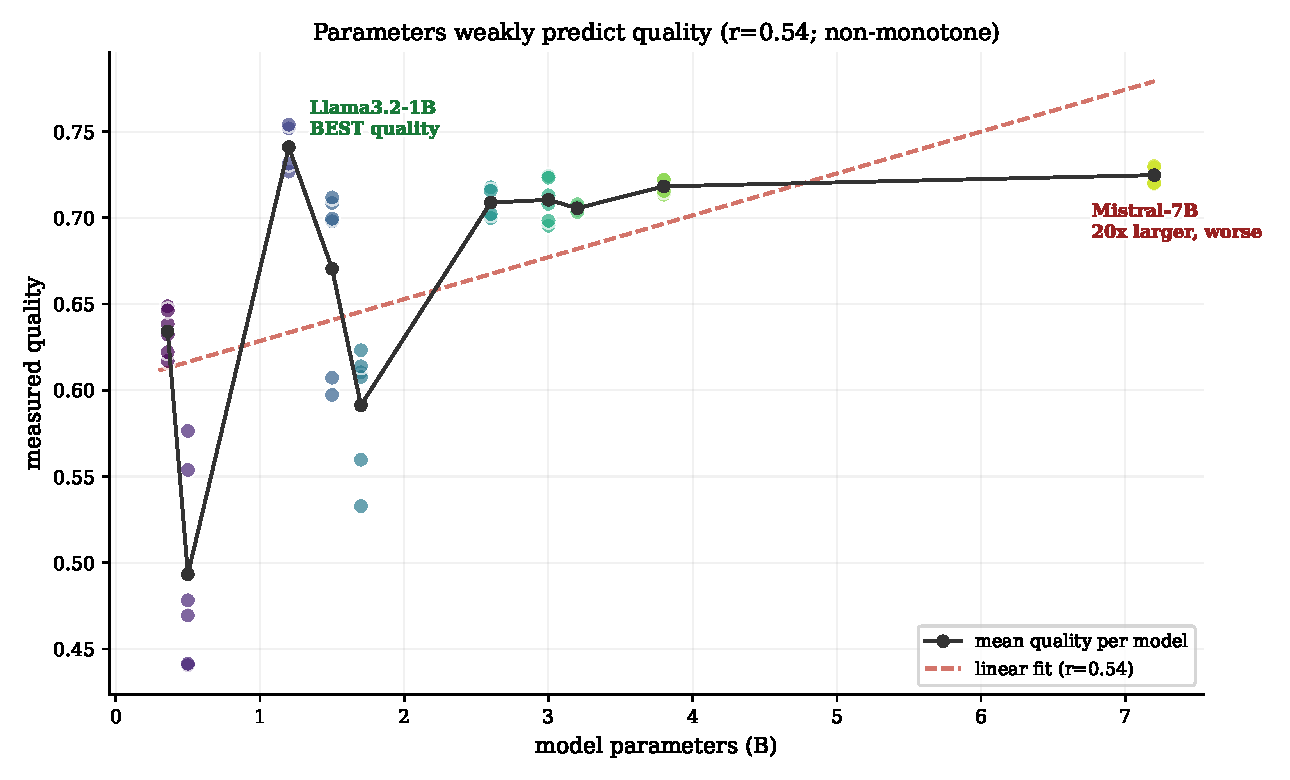
\includegraphics[width=0.92\textwidth]{fig/q2_params_quality.pdf}
\caption{Measured specialist quality versus parameter count. The per-model mean
(black) is non-monotone; the linear fit is weak ($r{=}0.54$). Llama-3.2-1B is the
best model overall, beating Mistral-7B at a fraction of the size.}
\label{fig:q_params}
\end{figure}

\subsection{The quality--latency frontier is dominated by small models}
Building the Pareto frontier of measured quality versus latency
(Fig.~\ref{fig:q_frontier}), \textbf{only $4$ of $50$ specialist configurations
are non-dominated, and none exceeds $1.2$\,B parameters}. Every large model
(Mistral-7B, Phi-3.5) is strictly dominated: it is matched or
beaten in quality by Llama-3.2-1B while costing $4$--$6\times$ the latency and up
to $6\times$ the VRAM. The quality frontier is therefore the near-opposite of the
parameter-capacity frontier of §\ref{sec:opt}.

\begin{figure}[H]
\centering
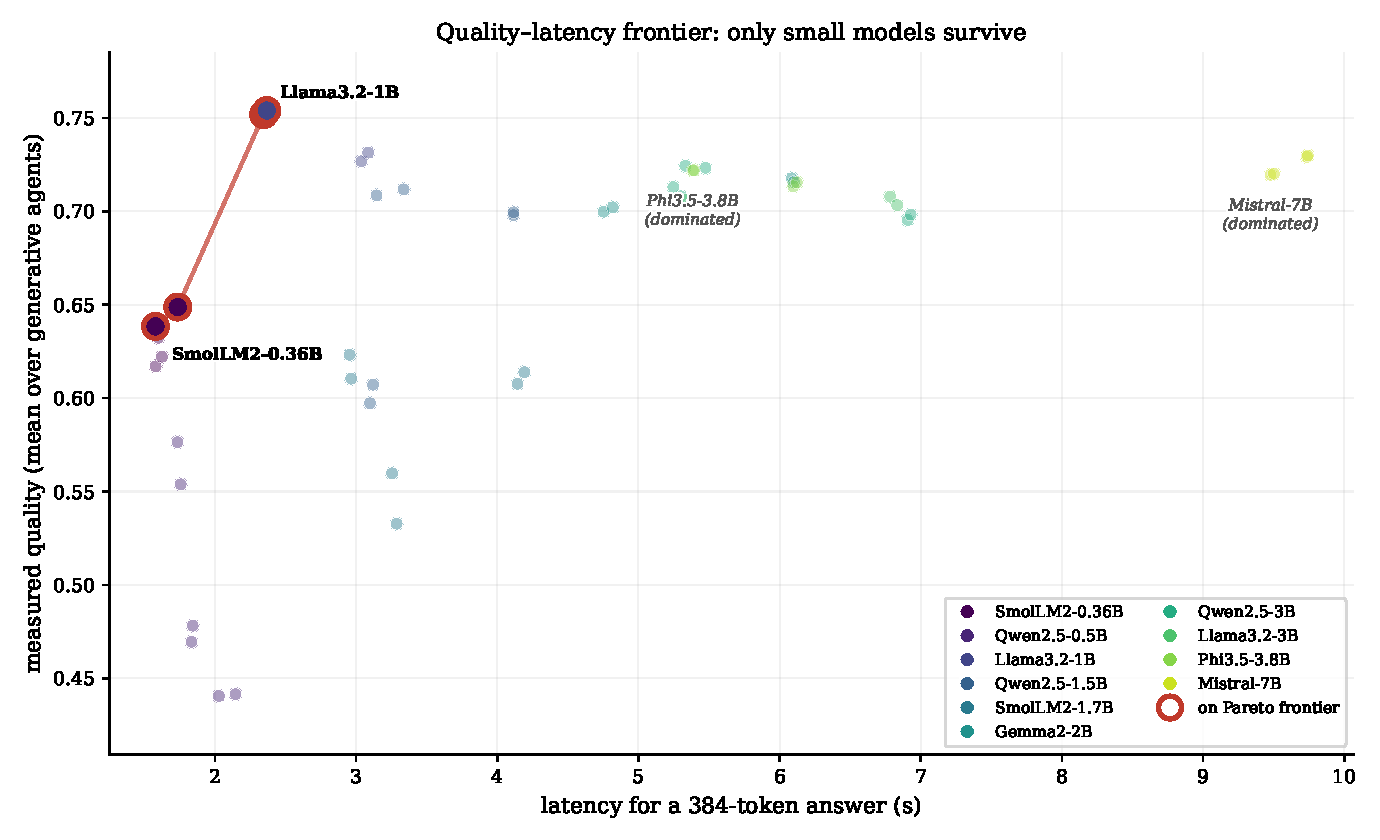
\includegraphics[width=\textwidth]{fig/q1_frontier_latency.pdf}
\caption{Measured quality versus latency for all specialist configurations. Only
four small-model configurations lie on the Pareto frontier (red rings); the large
models sit in the dominated upper-right region (same quality, far higher latency).}
\label{fig:q_frontier}
\end{figure}

\subsection{Validation: the highest-capacity allocation is sub-optimal in quality}
\label{sec:quality-validation}
We can now validate the parameter-proxy allocator directly. For each latency
budget we compare the model the capacity-maximizing policy (§\ref{sec:opt}) would
place in the specialist slot against the measured-quality-optimal choice
(Fig.~\ref{fig:q_policy}). The capacity policy is \textbf{sub-optimal at every one
of the $105$ budget steps tested}, by a mean of $0.051$ and up to $0.131$ quality
points. As the budget grows it spends the extra latency on ever-larger models
(SmolLM2-1.7B\,$\to$\,Gemma-2\,$\to$\,Phi-3.5\,$\to$\,Mistral-7B) without ever
matching the quality that Llama-3.2-1B delivers cheaply. This is direct,
measured evidence that maximizing capacity (or parameters) is the wrong
objective, and it quantifies the quality left on the table by a proxy-based
allocator---the gap a quality-aware MILP would close.

\begin{figure}[H]
\centering
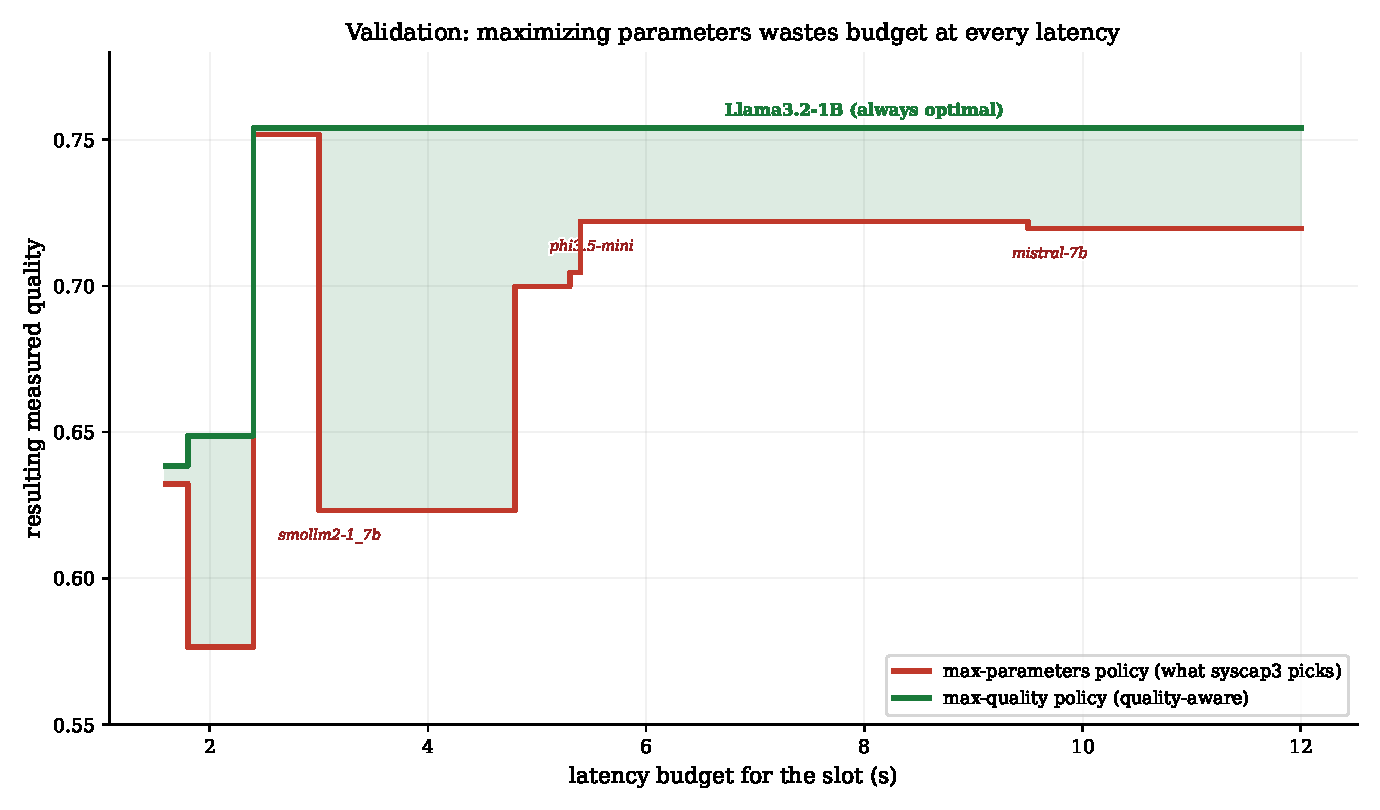
\includegraphics[width=\textwidth]{fig/q3_policy_compare.pdf}
\caption{Validation of the capacity proxy. At each latency budget, the
quality of the model chosen by the capacity-maximizing policy (red) versus the
measured-quality-optimal model (green). The capacity policy is dominated at every
budget; the shaded region is the quality forgone.}
\label{fig:q_policy}
\end{figure}

\subsection{Held-out validation: the small-specialist finding is not in-sample overfitting}
\label{sec:quality-heldout}
The quality-aware allocator selects the specialist using measured quality, and a
fair objection is that the resulting choice could be over-fit to the small
evaluation set---the reported quality being optimistic because the same queries
both select and score the model. We test this with a \emph{leave-one-domain-out}
(LODO) protocol, which is stricter than a random query split because it withholds an
entire legal domain: for each of the nine domains in turn, we select the
best specialist model using only the queries of the \emph{other eight} domains, then
evaluate that model on the held-out domain it was not allowed to see.

The finding survives the split cleanly. The model selected on the training domains
is Llama-3.2-1B in \textbf{$9$ of $9$ folds}; the choice never depends on the
held-out domain. Its held-out quality tracks the per-fold oracle (the best model
chosen \emph{with} access to the held-out domain) almost exactly---a mean
generalization gap of $0.001$ and at most $0.008$ quality points across all folds.
And the small-model advantage itself generalizes: on the held-out domain the
train-selected Llama-3.2-1B beats Mistral-7B in $7$ of $9$ folds (mean $+0.018$),
losing narrowly only on the two domains where a larger model is genuinely best
(family mediation and consensual separation, both Mistral-7B), consistent
with the per-domain heterogeneity reported next. The quality-aware optimum is
therefore a property of the measured data, not an artifact of selecting and scoring
on the same queries; the residual caveat is the absolute sample size
(§\ref{sec:limits}), not the selection procedure.

\subsection{Specialist evaluation by domain}
The nine specialists cover distinct legal domains, and the best model differs by
domain (Fig.~\ref{fig:q_matrix})---the structural premise of the heterogeneous
formulation (§\ref{sec:opt}), now measured rather than synthetic. Llama-3.2-1B is
the best specialist in $7$ of $9$ domains, but not all: family mediation
(\emph{negoziazione}) and consensual separation are both best served by
Mistral-7B. The quality spread across models within a domain is large (e.g.\
$0.47$--$0.76$ for \emph{volontaria giurisdizione}), confirming that model choice
per domain matters and is not reducible to a single ranking.

\begin{figure}[H]
\centering
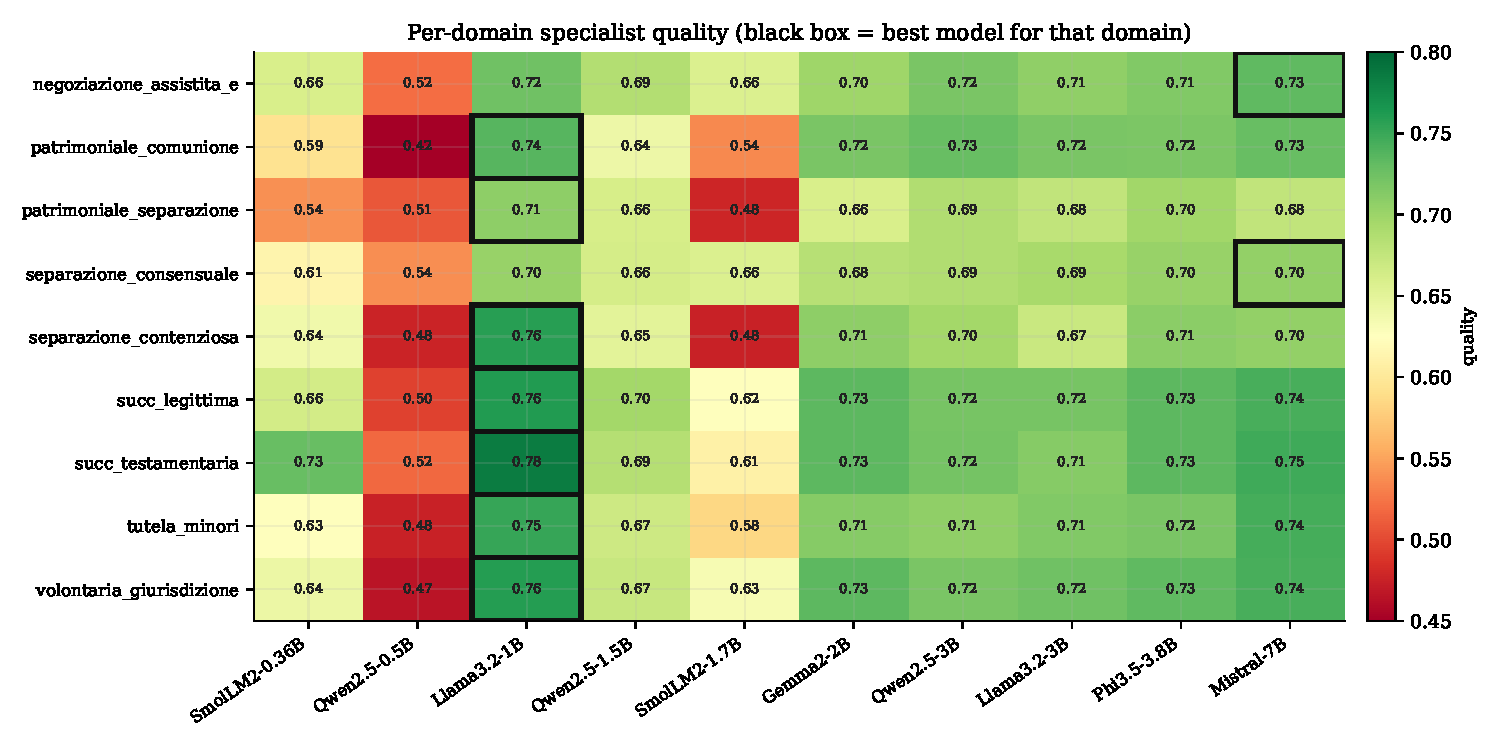
\includegraphics[width=\textwidth]{fig/q6_agent_matrix.pdf}
\caption{Per-domain specialist quality for every model (black box = best model in
that domain). Llama-3.2-1B (the strong column) wins most domains; Mistral-7B
wins the other two, illustrating genuine per-domain heterogeneity.}
\label{fig:q_matrix}
\end{figure}

\textbf{Statistical caveat (small per-domain samples).} These per-domain rankings
rest on few queries each: only $2$ of the $9$ domains
(\emph{succ.\ legittima}, $n{=}22$; \emph{succ.\ testamentaria}, $n{=}14$) have
$n\ge 10$; the other $7$ have $n\in\{3,\dots,9\}$. We therefore report
$95\%$ bootstrap confidence intervals on each domain's best-model quality
(Fig.~\ref{fig:domain_ci}) and flag the under-powered domains explicitly. The
intervals are wide where $n$ is small (e.g.\ \emph{separazione contenziosa},
$n{=}4$, CI $[0.68,0.83]$), so individual per-domain ``best model'' claims with
$n<10$ should be read as suggestive, not conclusive. The \emph{pooled} signal is
nonetheless strong: pooled over Llama-3.2-1B's $282$ specialist records (of
$3439$ in total), its lead is tight (CI $[0.743,0.764]$), and it is the best or
statistically-tied model in $7$ of $9$ domains. The robust claim is the pooled and
cross-role one (the three regimes); the per-domain winners are indicative.

\begin{figure}[H]
\centering
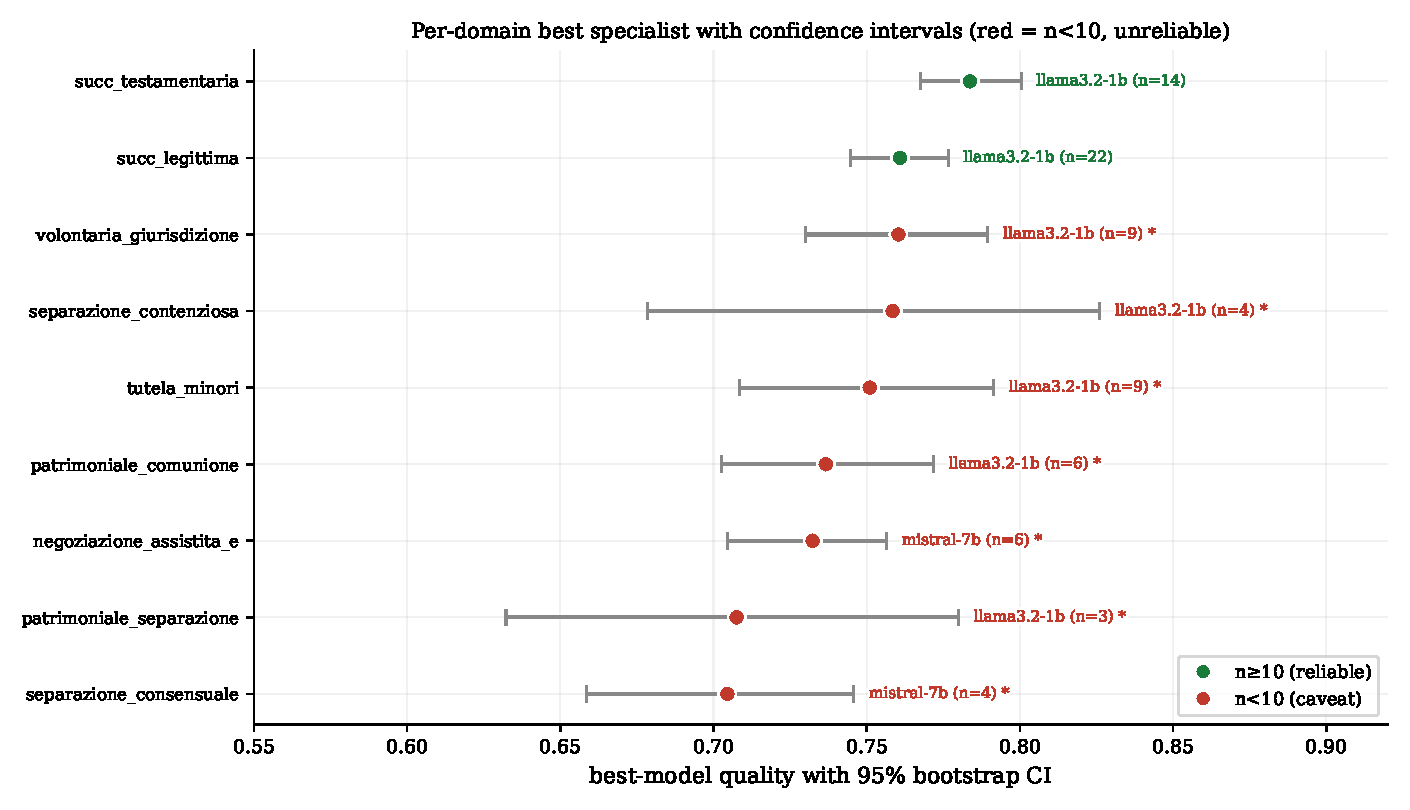
\includegraphics[width=\textwidth]{fig/q12_per_domain_ci.pdf}
\caption{Per-domain best-specialist quality with $95\%$ bootstrap confidence
intervals. Green = $n\ge 10$ (reliable); red = $n<10$ (caveat). Intervals widen
sharply at small $n$; the pooled specialist signal (not shown here) is far
tighter.}
\label{fig:domain_ci}
\end{figure}

\subsection{Dispatcher evaluation: routing F1 rewards larger models}
The dispatcher is scored by routing F1 (predicted vs.\ expected specialist set).
Routing quality increases with model size (Fig.~\ref{fig:q_dispatcher}), led by
Phi-3.5 ($0.65$), Mistral-7B ($0.59$), and Gemma-2 ($0.57$), while the sub-$2$\,B
models trail at $0.18$--$0.39$. One model is excluded from the trend reading:
across its $312$ dispatcher records, Llama-3.2-3B emits a \emph{constant}
specialist set independent of the query, a routing-format failure that yields
$F_1{=}0.06$---a degenerate outlier, not a noisy estimate. Routing---a short,
structured classification over the query---benefits from larger models, the
opposite of the generative specialist role.

\begin{figure}[H]
\centering
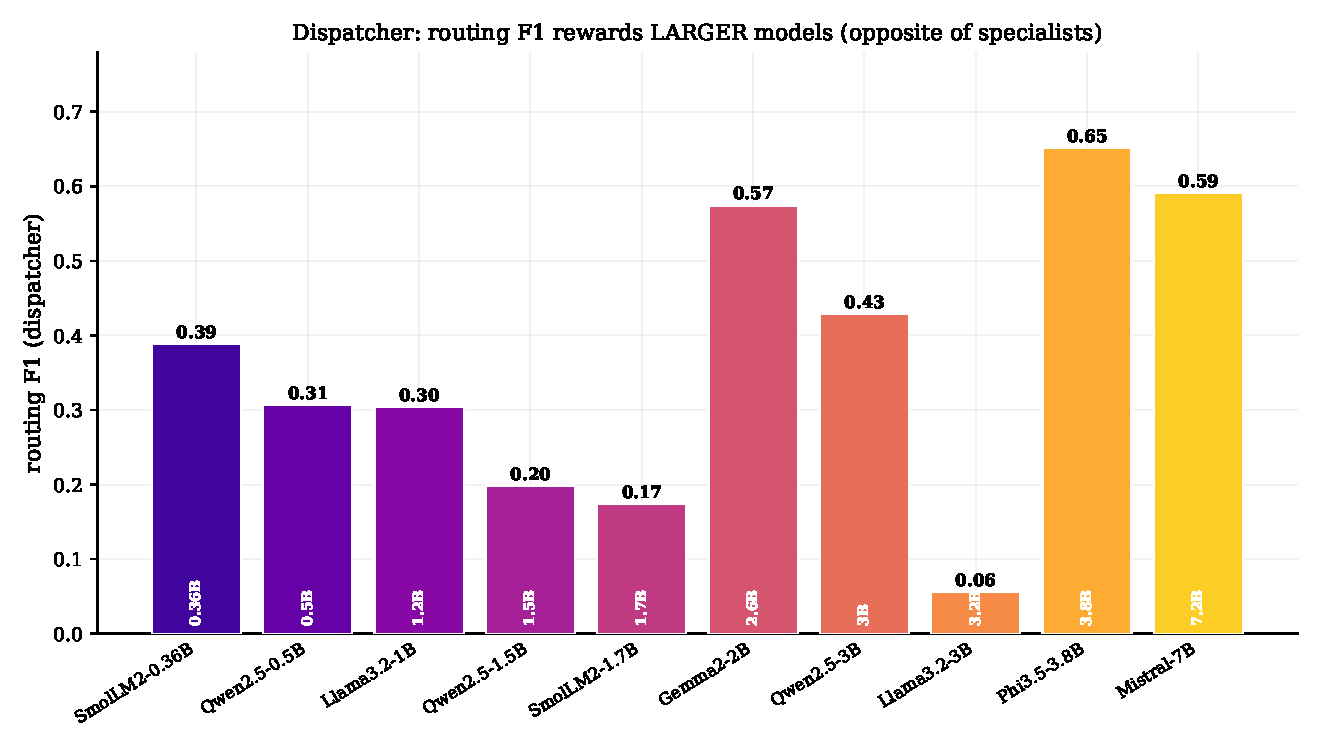
\includegraphics[width=0.92\textwidth]{fig/q5_dispatcher_f1.pdf}
\caption{Dispatcher routing F1 by model. Unlike the specialists, routing quality
rises with size (Phi-3.5 and Mistral-7B lead). (Llama-3.2-3B is a degenerate
outlier: it routes every query to the same fixed specialist set; see text.)}
\label{fig:q_dispatcher}
\end{figure}

\subsection{Synthesiser evaluation: quality rises with size}
\label{sec:quality-synth}
The synthesiser pass is now sufficiently advanced to analyze ($620$ scored
records over $25$ configurations and all $25$ calibration queries). Its behaviour
is the \emph{opposite} of the specialists' and matches the dispatcher's: synthesis
quality rises with model size, nearly monotonically (Fig.~\ref{fig:q_synth}), and
the best synthesiser is the largest model, \textbf{Mistral-7B} (quality $0.77$),
ahead of Phi-3.5 ($0.73$) and Gemma-2 ($0.72$), with the sub-$2$\,B models
trailing at $0.58$--$0.65$. Composing a coherent final answer from several
specialist outputs evidently benefits from a larger model, much as routing does.

\begin{figure}[H]
\centering
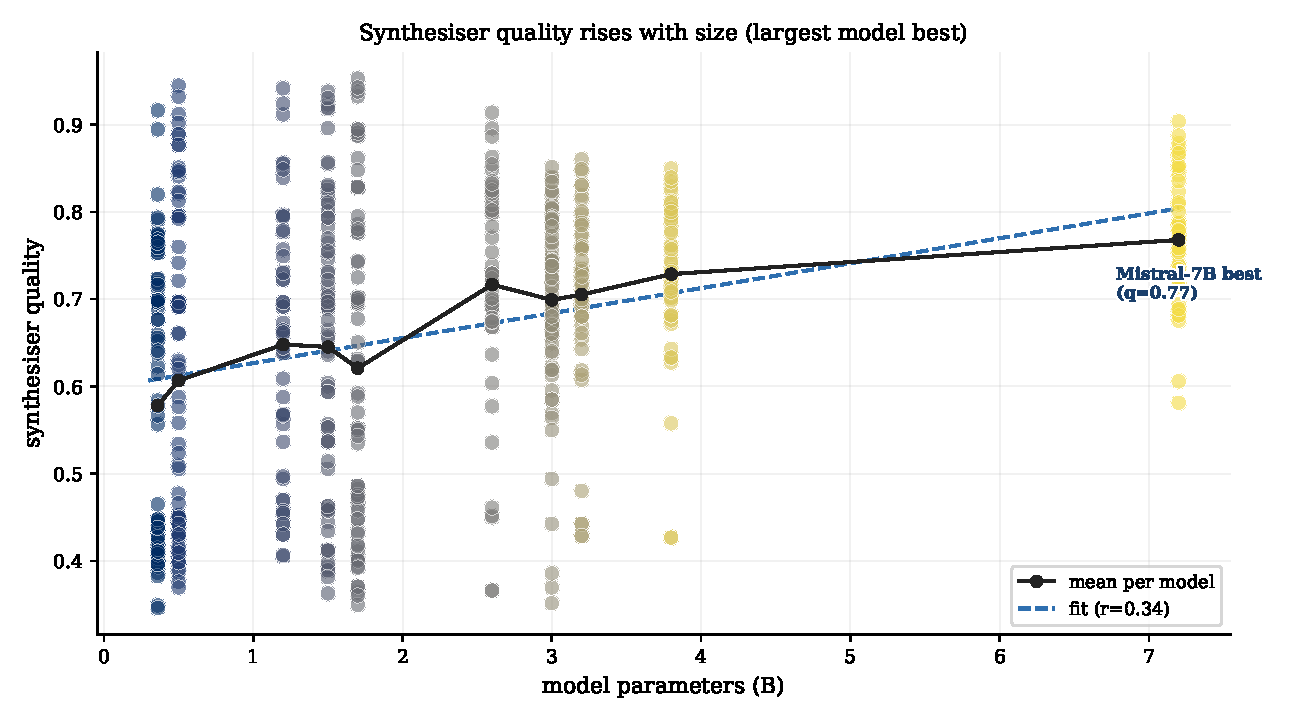
\includegraphics[width=0.92\textwidth]{fig/q8_synth_quality.pdf}
\caption{Synthesiser quality versus parameter count ($620$ records). Quality
rises with size (per-model mean in black); the largest model, Mistral-7B, is
best. This is the reverse of the specialists and parallels the dispatcher.}
\label{fig:q_synth}
\end{figure}

\textbf{Decomposing the synthesiser metric.} The aggregate hides a more
informative structure (Fig.~\ref{fig:q_synth_ragas}). Of the five components,
\emph{context precision} and \emph{context recall} are \textbf{constant across all
synthesiser models} ($0.82$ and $0.52$): under the oracle-retrieval evaluation
(§\ref{sec:setting-retrieval}) the contexts are the gold passages, supplied
identically to every model, so these retrieval metrics depend on the context set,
not the generative model. The aggregate quality is driven almost entirely
by \emph{correctness} (correlation $\approx 1.0$ with the aggregate) and
\emph{answer relevancy}, both of which rise with model size. Strikingly,
\emph{faithfulness moves in the opposite direction}---it \textbf{falls} as models
grow (correlation $-0.70$ with quality). The larger synthesisers are less faithful
to the supplied context yet more correct overall, indicating they lean on
parametric (in-weights) knowledge rather than the provided passages. For a legal
assistant this is a double-edged property---higher correctness but weaker
grounding---and it is invisible to the aggregate score alone.

\begin{figure}[H]
\centering
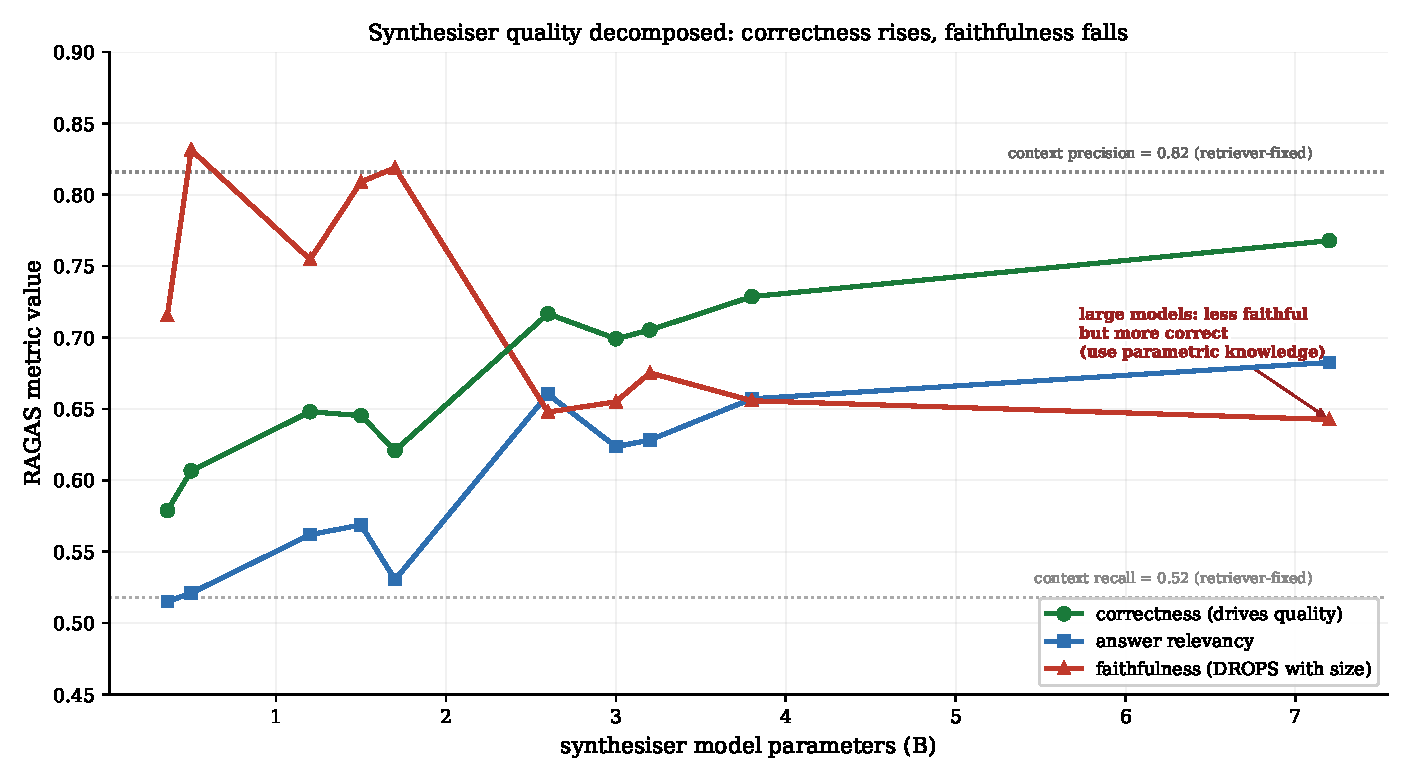
\includegraphics[width=0.92\textwidth]{fig/q10_synth_ragas.pdf}
\caption{Synthesiser quality decomposed into RAGAS components. Correctness and
answer relevancy rise with size; faithfulness \emph{falls} (larger models rely on
parametric knowledge); context precision/recall are retriever-fixed constants. The
aggregate is correctness-dominated.}
\label{fig:q_synth_ragas}
\end{figure}

\subsection{The central finding: three roles, three scaling laws}
\label{sec:quality-three}
Putting the three roles together yields the paper's sharpest allocation insight
(Fig.~\ref{fig:q_three}). The \emph{dispatcher} (routing) and the
\emph{synthesiser} (composition) both improve with model size and are best served
by the \emph{largest} models that fit. The \emph{specialists} (domain-grounded
RAG) do not: their quality peaks at Llama-3.2-1B and then plateaus, so they are
best served by \emph{small} models. The three roles therefore demand models from
opposite ends of the size spectrum simultaneously. No single global rule
(``largest that fits'' or ``smallest that fits'') is correct for the pipeline;
only a \emph{per-role} allocator can place a large dispatcher and synthesiser
alongside small specialists---which is precisely the structure the MILP encodes.
This is the measured justification for role-aware allocation, and it is the
strongest argument in the paper that the optimization problem is real.

\begin{figure}[H]
\centering
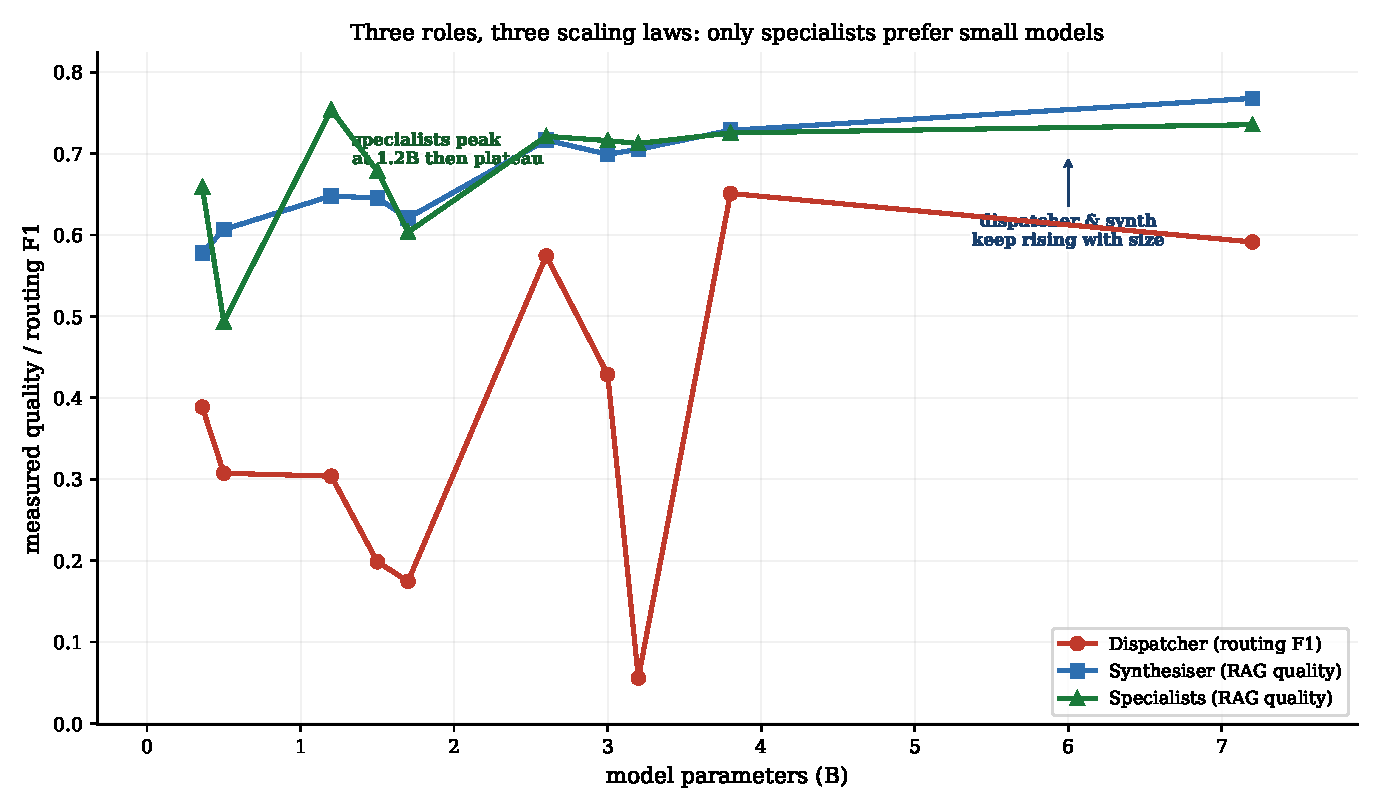
\includegraphics[width=\textwidth]{fig/q7_three_regimes.pdf}
\caption{Measured quality versus model size for the three roles. Dispatcher
(routing F1) and synthesiser (RAG quality) rise with size; specialists peak at
$1.2$\,B and plateau. The roles prefer opposite ends of the size range, which a
per-role allocator can exploit. The dispatcher curve is noisier (e.g.\
the degenerate Llama-3.2-3B outlier, \S\ref{sec:quality}); the trend is
nonetheless clear.}
\label{fig:q_three}
\end{figure}

\subsection{Why three regimes? A mechanistic account}
\label{sec:quality-why}
The three scaling laws are not arbitrary; they follow from what each role's task
demands of a model, and the RAGAS decomposition (§\ref{sec:quality-synth}) supplies
direct evidence. We offer the following account, which turns the empirical finding
into a \emph{predictive} hypothesis.

\textbf{The governing variable is how much the task rewards parametric knowledge
versus penalizes it.} A model's quality on a task is, loosely, a sum of two
size-dependent effects: larger models bring more parametric knowledge and stronger
reasoning (helps), but they also drift further from a short supplied context when
left unconstrained (can hurt grounding). The balance differs by role:

\begin{itemize}\itemsep2pt
\item \textbf{Dispatcher (routing) --- rewards scale.} Routing is short structured
classification over the query: no long generation, nothing to hallucinate, and the
decision benefits from broad world/linguistic knowledge to disambiguate domains.
The penalty term is essentially absent (there is no context to be unfaithful to),
so quality is increasing in size. Hence routing F1 rises with parameters.
\item \textbf{Specialist (domain-grounded RAG) --- penalizes scale past a point.}
The specialist must answer \emph{from the retrieved legal passage}. Here the two
effects oppose: a little more capability helps, but larger models increasingly
substitute parametric (and possibly wrong or generic) knowledge for the supplied
article, which on narrow legal questions is a net negative. The measured signature
is exactly this: for the synthesiser we observe correctness rising while
\emph{faithfulness falls} with size (§\ref{sec:quality-synth}); the specialists,
whose entire job is grounding, hit the crossover earlier---quality peaks at
$\approx1.2$\,B and plateaus. Small grounded models win because the task rewards
fidelity to context over recall of weights.
\item \textbf{Synthesiser (composition) --- rewards scale, but less cleanly.}
Composing several specialist answers into a coherent whole is a longer generative
task that benefits from fluency and reasoning (helps, like routing), yet it also
shows the falling-faithfulness signature (like the specialists). The first effect
dominates over our range, so quality rises with size, but more slowly and less
monotonically than routing---which is what the curve shows.
\end{itemize}

\textbf{The prediction.} This account is falsifiable and portable: a role's optimal
model size should track its \emph{grounding requirement}. Tasks that must be
faithful to a short supplied context (extraction, grounded QA, citation) should
favour small models and exhibit an early quality peak; tasks that are
classification-like or that legitimately draw on parametric knowledge (routing,
open-domain synthesis, summarization without a single source of truth) should favour
larger models. A direct test is to manipulate the grounding requirement---e.g.\
shrink or remove the retrieved context---and predict that the specialist's optimal
size \emph{increases} as grounding is weakened, because the penalty term vanishes.
We do not run that ablation here; it is the natural next experiment, and the point
is that the three-regime finding now comes with a mechanism that says \emph{when} to
expect each regime, not merely that we observed three.

\subsection{Retriever diagnostic}
\label{sec:quality-retriever}
Separately from the oracle-retrieval quality scores, we evaluate the \emph{live}
FAISS retriever (§\ref{sec:setting-retrieval}) against the gold authority ids.
Across query--specialist pairs, context recall is frequently low
($0.17$--$0.43$ on many queries) and---crucially---\emph{identical for the
specialist and the synthesiser on the same query}, because both consume the same
retrieved passages. Retrieval quality is therefore a system-level bottleneck
independent of which generative models are allocated: no model choice can recover
information the retriever failed to surface. This bounds the achievable pipeline
quality and is an orthogonal target for future improvement (better chunking,
embeddings, or reranking), separate from the allocation problem studied here.

\section{Quality-Aware Allocation}
\label{sec:qmilp}
\emph{This section closes Q2: having shown the proxy is the wrong objective, we put
measured quality \emph{inside} the optimizer and compare.}
The measured results motivate replacing the parameter proxy with measured quality
\emph{inside} the optimizer. We now do so, giving the quality-aware counterpart of
the MILP in §\ref{sec:milp} and the resulting measured frontier. This is the
paper's culminating result: an allocator that maximizes \emph{measured} pipeline
quality, and a direct demonstration that it departs from the parameter-proxy
optimum.

\subsection{Formulation}
The structure is identical to §\ref{sec:milp}---three role-slots, load-once
memory, serial latency---but the objective is the measured pipeline quality.
Let $Q^{\mathrm{F1}}_c$ be the dispatcher's measured routing F1 for configuration
$c$, $Q^{\mathrm{syn}}_c$ the synthesiser's measured quality, and
$\bar Q^{\mathrm{spec}}_c$ the specialist model's measured quality averaged over
the activated domains. With role-slot assignment variables $x_{d,c},x_{s,c},x_{y,c}$
and loaded-config variables $z_c$ as before:
\begin{equation}
\max\ \ w_d \!\sum_c Q^{\mathrm{F1}}_c x_{d,c}
\;+\; \sum_c \bar Q^{\mathrm{spec}}_c x_{s,c}
\;+\; w_y \!\sum_c Q^{\mathrm{syn}}_c x_{y,c}
\label{eq:qobj}
\end{equation}
subject to one configuration per role
($\sum_c x_{r,c}{=}1$), load-only-if-used ($x_{r,c}\le z_c$), one context per
weight-sharing group, the load-once memory budget
$\sum_c \mu_c z_c \le M$, and the serial latency chain
\begin{equation}
\sum_c \ell^{\mathrm{r}}_c x_{d,c} + k\!\sum_c \ell^{\mathrm{g}}_c x_{s,c}
+ \sum_c \ell^{\mathrm{g}}_c x_{y,c} \le \eps .
\label{eq:qlat}
\end{equation}
We set $w_d{=}0.15$ (routing weighted below generation) and $w_y{=}1$; the
weights are a modelling choice, stated as such. The program is linear and solves
in well under a second.

\textbf{Scope and assumptions.} This objective is \emph{additive} across roles: it
sums the three measured qualities and does not model the router-gating interaction
(a specialist's contribution being wasted when the router misroutes), which in the
full system is a bilinear term. The specialist quality is the model's mean over
activated domains (the shared-specialist abstraction of §\ref{sec:milp}), and the
synthesiser quality is measured against fixed reference specialist answers
(§\ref{sec:quality}), so it is independent of the allocation and keeps the program
linear. We keep this additive form as the primary allocator for clarity, and then
\emph{relax the additivity}---adding the measured bilinear router--specialist
gating---in §\ref{sec:bilinear}, which shows the coupling changes the optimal
allocation.

\subsection{The measured quality--latency frontier}
Solving \eqref{eq:qobj}--\eqref{eq:qlat} over a sweep of $\eps$ for each $k$ yields
the measured quality--latency frontier (Fig.~\ref{fig:qfrontier}). The optimizer,
given only measured quality, \emph{independently recovers the three-regime
structure}: at essentially every budget it selects a \textbf{large dispatcher
(Mistral-7B), a small specialist (Llama-3.2-1B), and a large synthesiser
(Mistral-7B)}. It was told nothing about roles preferring different sizes; it
reconstructs that pattern purely by maximizing measured quality under the
constraints. The frontier plateaus near $Q{=}1.60$ once the budget admits this
mixed allocation.

\begin{figure}[H]
\centering
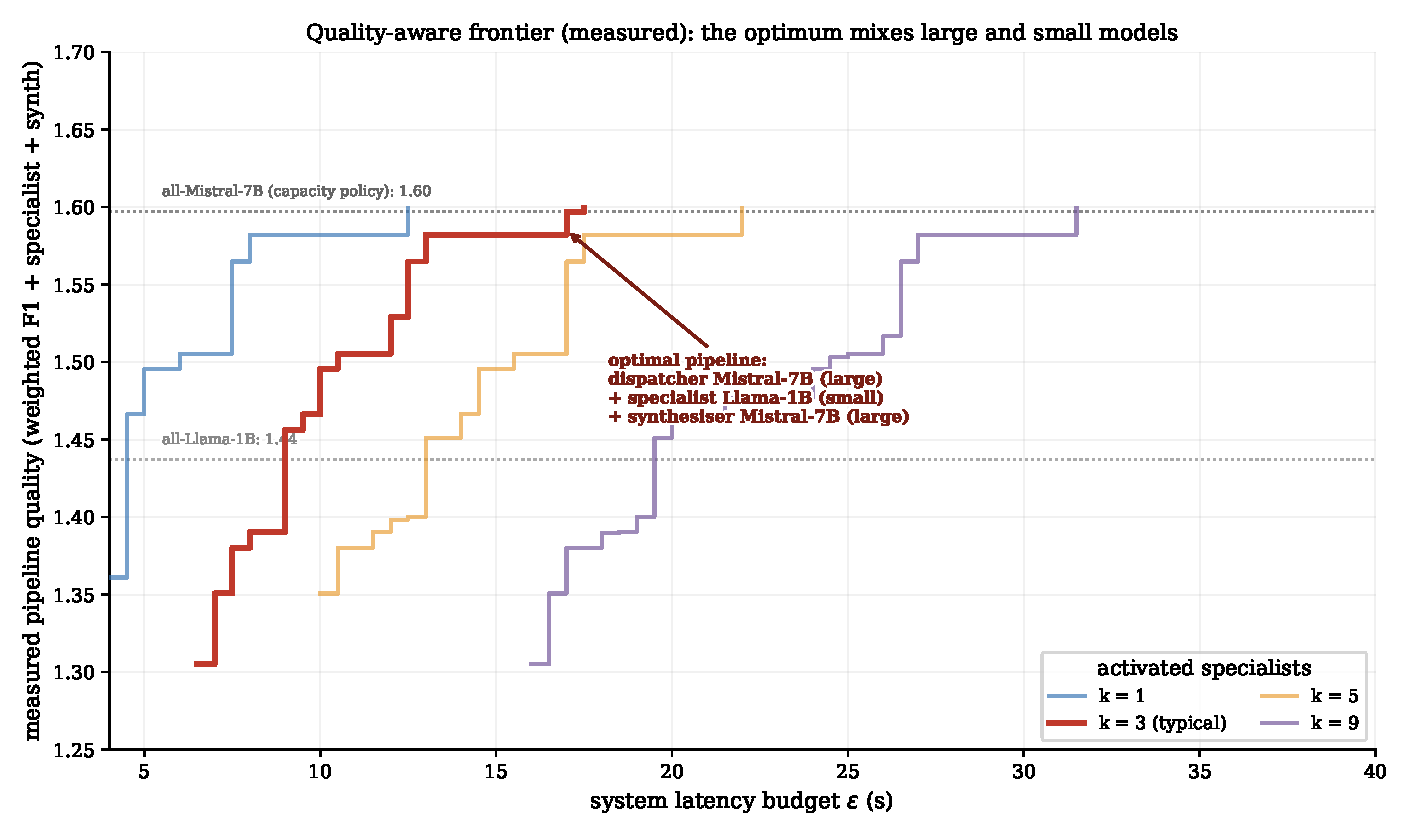
\includegraphics[width=\textwidth]{fig/q9_quality_frontier.pdf}
\caption{Measured quality--latency frontier from the quality-aware MILP, for
$k\in\{1,3,5,9\}$. The optimal allocation mixes model sizes---large dispatcher and
synthesiser, small specialist---recovering the three-regime structure from data.
Dotted lines mark two fixed-model policies, both dominated.}
\label{fig:qfrontier}
\end{figure}

\subsection{Optimization beats fixed policies and the parameter proxy}
Two comparisons establish that the quality-aware optimization is necessary, not
cosmetic. First, against \emph{fixed-model} policies at $k{=}3$: the mixed optimum scores
$Q{=}1.60$, against $1.60$ for the best single all-Mistral-7B configuration and
$1.44$ for all-Llama-3.2-1B. We report this honestly: an \emph{unconstrained}
all-Mistral policy nearly ties the mixed optimum ($\Delta{=}0.002$), because
Mistral is also the best routing and synthesis model---but only at the far right
of the latency axis, where its full sequential chain is affordable. The decisive
comparison is therefore at \emph{matched latency}. Second, and most directly,
against the \emph{parameter-proxy} allocator of §\ref{sec:opt}: at matched latency
the proxy is sub-optimal at \textbf{every one of the $26$ budgets tested}, by a
mean of $0.13$ and up to $0.18$ quality points (Fig.~\ref{fig:proxy_quality})---a
gap several times larger than the proxy's gap against a greedy sort
(§\ref{sec:opt}). The proxy's failure is mechanistic: maximizing parameters spends
the latency budget on a large dispatcher and is then forced onto small specialist
\emph{and} synthesiser models, so its quality can even \emph{decrease} as the
budget grows. This is the quantitative core of the paper's thesis: \textbf{a
parameter proxy and a measured-quality objective induce materially different
optimal configurations}, and only the latter tracks what the system actually
delivers.

\begin{figure}[H]
\centering
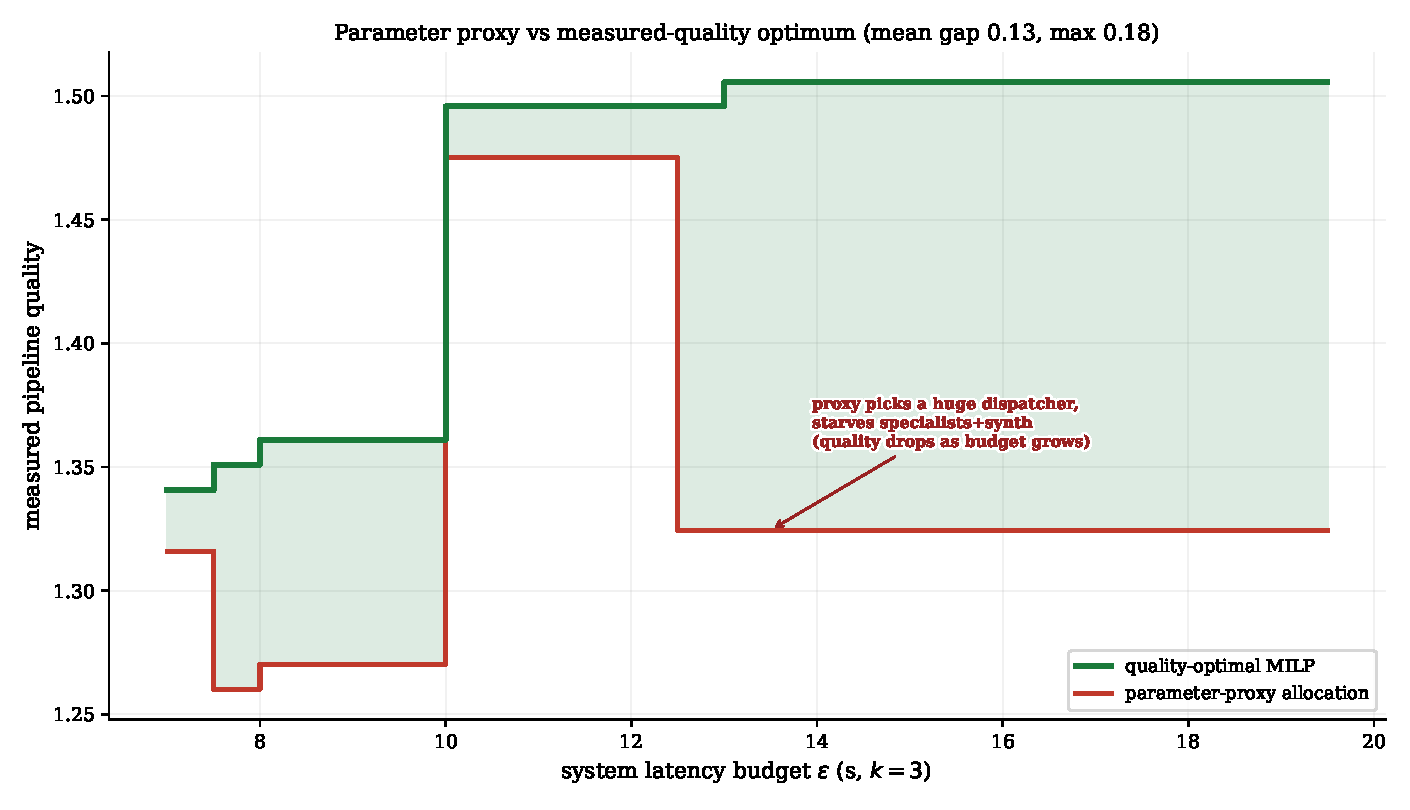
\includegraphics[width=\textwidth]{fig/q11_proxy_vs_quality.pdf}
\caption{Parameter-proxy allocation versus the measured-quality optimum at matched
latency ($k{=}3$). The proxy is dominated at every budget (mean gap $0.13$, max
$0.18$) and is non-monotone---spending budget on a large dispatcher starves the
other roles. Measured quality and the parameter proxy yield different optima.}
\label{fig:proxy_quality}
\end{figure}

\textbf{Robustness to the objective weights.} Because $w_d$ and $w_y$ are a
modelling choice, we re-solve the quality-aware MILP across a grid
$w_d\in\{0.05,0.15,0.30,0.50,1.0\}$, $w_y\in\{0.5,1.0,1.5\}$ (at $\eps{=}15$,
$k{=}3$). The qualitative conclusion is invariant: in \textbf{all $15$ weight
combinations the optimal specialist is the small Llama-3.2-1B while the dispatcher
and synthesiser remain large} (Fig.~\ref{fig:weight_sens}). The mixed
large/small/large structure---and hence the departure from the parameter
proxy---is therefore not an artifact of the chosen weights; only the second-order
choice between the large models (Phi-3.5 vs Mistral-7B) shifts with the weighting.

\begin{figure}[H]
\centering
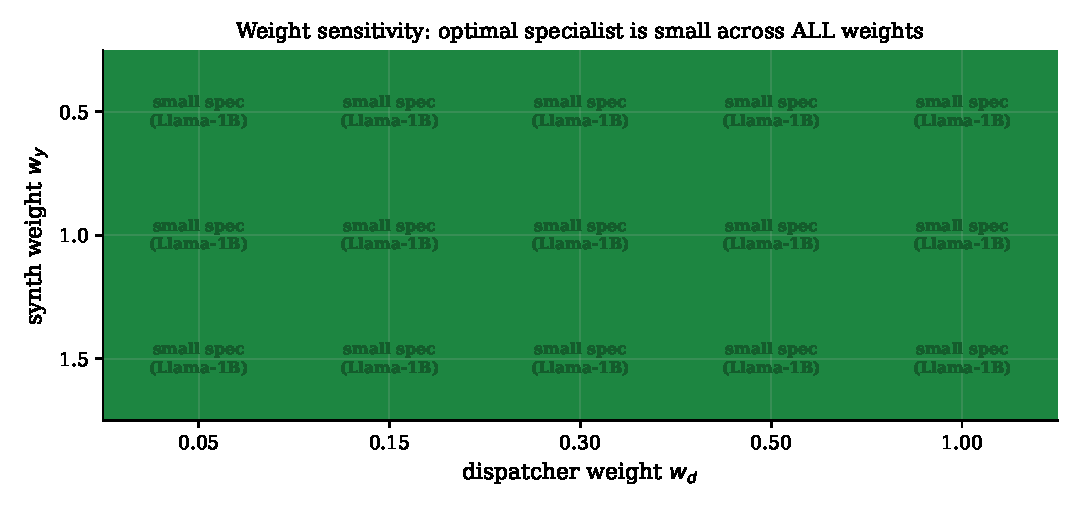
\includegraphics[width=0.82\textwidth]{fig/q13_weight_sensitivity.pdf}
\caption{Weight sensitivity of the quality-aware optimum ($\eps{=}15$, $k{=}3$).
Across the full $w_d\times w_y$ grid the optimal specialist is always the small
Llama-3.2-1B (dispatcher and synthesiser stay large), so the qualitative
conclusion is weight-robust.}
\label{fig:weight_sens}
\end{figure}

\section{Gated Allocation: Modelling Router--Specialist Coupling}
\label{sec:bilinear}
\emph{This section answers Q3: do the roles interact, and when does modelling that
interaction change the answer?}
The quality-aware objective~\eqref{eq:qobj} is \emph{additive}: it sums the three
roles' qualities as if independent. The real pipeline is not. A specialist's
answer is produced \emph{only if the dispatcher routes the query to it}; a
misroute wastes the specialist entirely, however good it is. The specialist's
effective contribution is therefore \emph{gated} by the dispatcher's routing
behaviour---a coupling between two allocation decisions. This is the genuinely
combinatorial core of the problem, and the reason a per-role sort cannot solve it.
The heterogeneous analysis of §\ref{sec:opt} modelled this coupling only on
\emph{synthetic} affinities; here we model it on \emph{measured} data and solve it
exactly.

\subsection{Measured routing recall}
From the dispatcher logs we estimate, for each dispatcher model $m$ and domain
$\delta$, the \textbf{per-domain routing recall}
\begin{equation}
\rho_{m,\delta}=\frac{\#\{\text{queries with }\delta\in\text{gold set, routed to }\delta\text{ by }m\}}
{\#\{\text{queries with }\delta\in\text{gold set}\}}\in[0,1].
\label{eq:recall}
\end{equation}
This is distinct from the global routing F1 of §\ref{sec:quality}: F1 averages over
\emph{all} domains, whereas $\rho_{m,\delta}$ is the recall on the specific domain
that will be activated. The two can diverge sharply---a model can have mediocre
global F1 yet excellent recall on a particular subset of domains
(Fig.~\ref{fig:bilinear}), and it is the latter that determines whether an
activated specialist is actually reached.

\subsection{Gated objective and exact linearization}
Let the dispatcher, specialist, and synthesiser model-choice indicators be
$y^{d}_{m}=\sum_{c:\,\mathrm{model}(c)=m}x_{d,c}$ (and likewise $y^{s}_{m}$,
$y^{y}_{m}$), each $\in\{0,1\}$ with $\sum_m y^{d}_m=1$. For the set $\mathcal A$
of activated domains, the \textbf{gated pipeline quality} is
\begin{equation}
Q_{\mathrm{gated}}=
w_d\, Q^{\mathrm{F1}}_{d}
+\frac{1}{|\mathcal A|}\sum_{\delta\in\mathcal A}\;
\underbrace{\Big(\sum_{m}\rho_{m,\delta}\,y^{d}_{m}\Big)}_{\text{router reaches }\delta}
\cdot
\underbrace{\Big(\sum_{m'}Q^{\mathrm{spec}}_{m',\delta}\,y^{s}_{m'}\Big)}_{\text{specialist quality on }\delta}
+\,w_y\, Q^{\mathrm{syn}}_{y}.
\label{eq:gated}
\end{equation}
The middle term is \textbf{bilinear}: it multiplies dispatcher indicators by
specialist indicators. We linearize it \emph{exactly} (binary $\times$ binary)
with McCormick envelopes. For each activated domain $\delta$ and model pair
$(m,m')$ with $\rho_{m,\delta}>0$ and $Q^{\mathrm{spec}}_{m',\delta}>0$, introduce
$w_{\delta,m,m'}\in[0,1]$ with
\begin{equation}
w_{\delta,m,m'}\le y^{d}_{m},\quad
w_{\delta,m,m'}\le y^{s}_{m'},\quad
w_{\delta,m,m'}\ge y^{d}_{m}+y^{s}_{m'}-1,
\label{eq:mccormick}
\end{equation}
which force $w_{\delta,m,m'}=y^{d}_{m}\,y^{s}_{m'}$ at any binary solution. The
gated term becomes the linear
$\sum_{\delta,m,m'}\rho_{m,\delta}\,Q^{\mathrm{spec}}_{m',\delta}\,w_{\delta,m,m'}/|\mathcal A|$,
so~\eqref{eq:gated} is a MILP under the same memory and latency constraints
(\eqref{eq:qlat}) and solves with CBC. Applying the envelopes at the
\emph{model} level (not configuration) keeps the auxiliary-variable count at
$|\mathcal A|\cdot|\mathcal M_d|\cdot|\mathcal M_s|\!\approx\!3\times11\times11$,
well within reach; a configuration-level encoding would be $\sim$$40\times$ larger
and is unnecessary because $\rho$ and $Q^{\mathrm{spec}}$ depend on the model, not
the quantization.

\subsection{Results: the coupling reshapes the optimum}
\textbf{Allocation.} Solved over the activated domains
(\emph{succ.\ legittima/testamentaria}, \emph{tutela minori}) at $k{=}3$, the gated
MILP selects a \emph{different} allocation from the additive one at every budget.
The change is concentrated, tellingly, in the \textbf{dispatcher}: the additive
model picks a high-global-F1 router (Phi-3.5, or Mistral-7B at large budgets),
whereas the gated model picks \textbf{SmolLM2-360M}---a router with low global F1
($0.39$) but near-perfect recall ($0.99$) on the activated domains
(Fig.~\ref{fig:bilinear}). The gated objective values recall \emph{on the domains
actually used}, and the tiny router additionally frees memory and latency for the
other roles. The specialist stays small (Llama-3.2-1B), consistent with the
three-regime finding: the coupling reshapes the \emph{dispatcher} decision,
exactly where the interaction lives.

\begin{figure}[H]
\centering
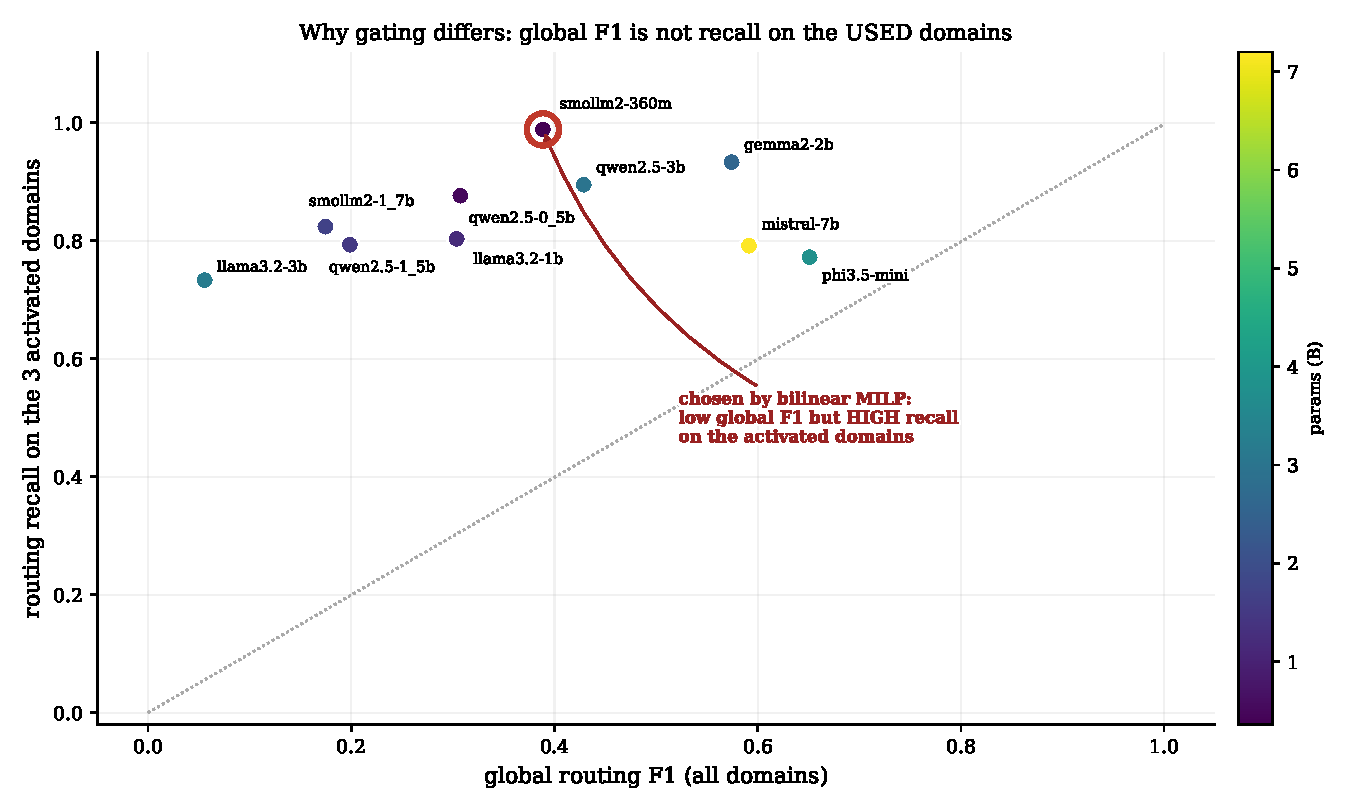
\includegraphics[width=\textwidth]{fig/q14_bilinear_recall.pdf}
\caption{Why gating changes the dispatcher choice. Each model's routing recall on
the three activated domains ($y$) exceeds its global F1 ($x$); that gap is what the
additive objective misses. SmolLM2-360M (circled) has low global F1 but the highest
activated-domain recall, so the gated MILP selects it. Colour is model size.}
\label{fig:bilinear}
\end{figure}

\textbf{Frontier.} Sweeping $\eps$ traces the gated quality--latency frontier
(Fig.~\ref{fig:bilinear_frontier}) for $k\in\{1,3,5\}$. It is the measured,
gated analogue of the capacity frontier of §\ref{sec:opt}: a staircase rising to a
plateau, but now in \emph{true pipeline quality} accounting for routing.

\begin{figure}[H]
\centering
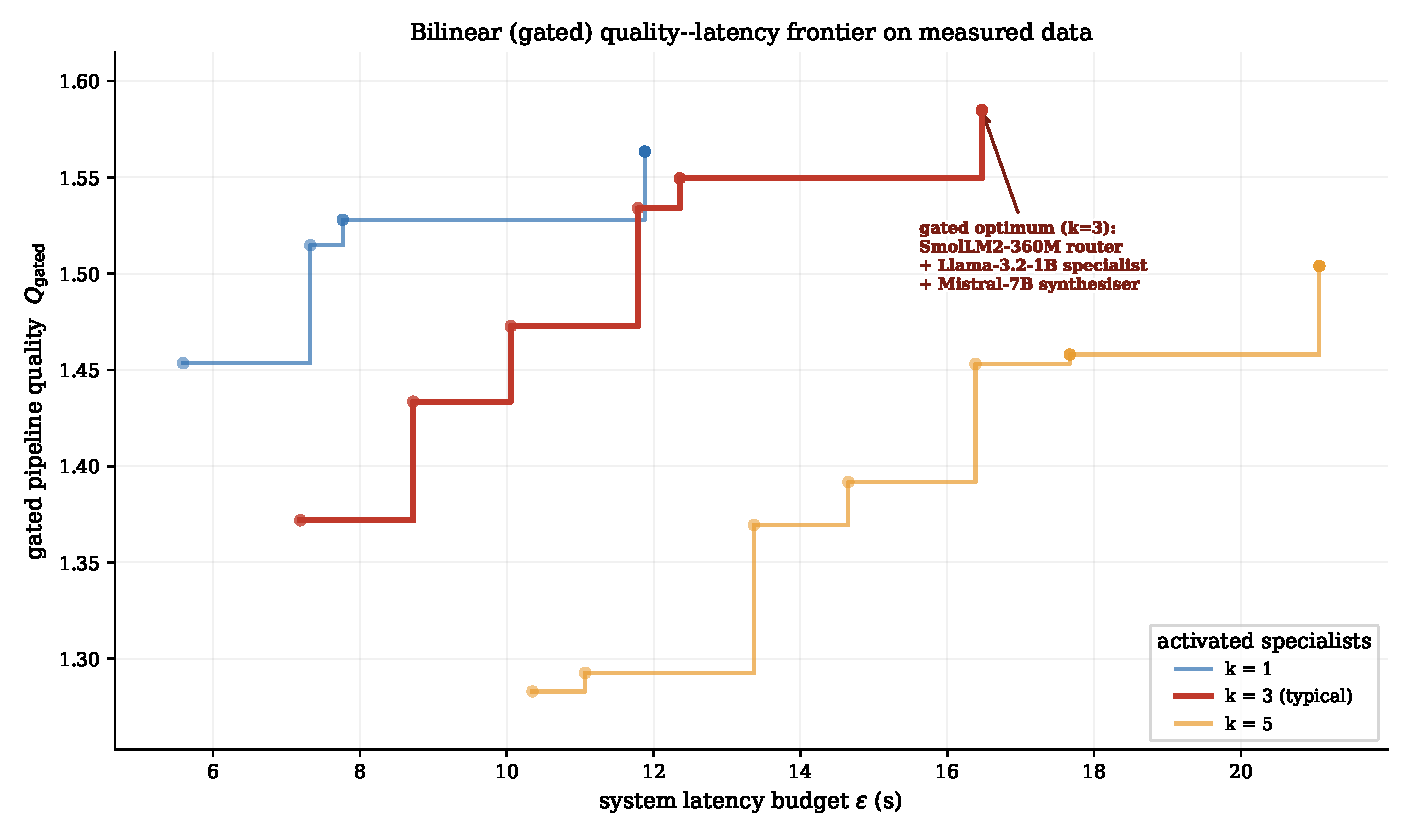
\includegraphics[width=\textwidth]{fig/q15_bilinear_frontier.pdf}
\caption{Gated quality--latency frontier from the bilinear MILP on measured data,
$k\in\{1,3,5\}$. Quality is $Q_{\mathrm{gated}}$ from~\eqref{eq:gated}; the
annotated $k{=}3$ optimum mixes a high-recall small router, a small specialist, and
a large synthesiser.}
\label{fig:bilinear_frontier}
\end{figure}

\textbf{Fair comparison.} To quantify the cost of ignoring the coupling, we take
the \emph{additive} optimum at each budget and re-score it under the \emph{true}
gating~\eqref{eq:gated}---i.e.\ we ask how the allocation that an additivity-blind
optimizer would deploy actually performs once the real router gates it. The gated
optimum dominates it at \textbf{42 of 44 budgets across $k\in\{1,3,5\}$}, by a mean
of $0.18$ and up to $0.32$ gated-quality points (Fig.~\ref{fig:bilinear_vs_add}).
The additive optimizer systematically over-values high-global-F1 routers that miss
on the activated domains, and under-values the small high-recall router the gated
model prefers.

\begin{figure}[H]
\centering
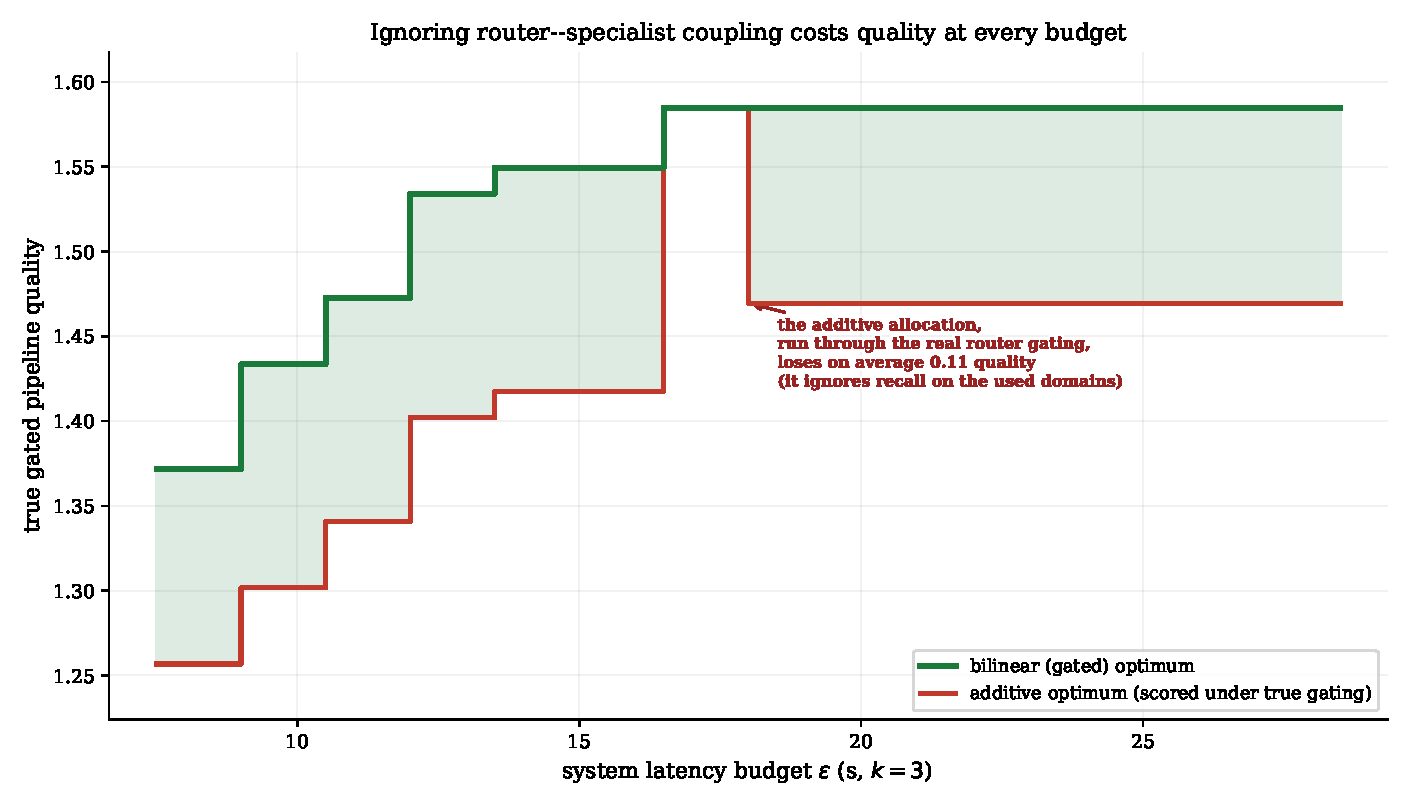
\includegraphics[width=\textwidth]{fig/q16_bilinear_vs_additive.pdf}
\caption{Cost of ignoring router--specialist coupling ($k{=}3$). Both allocations
are scored under the \emph{true} gating: the bilinear optimum (green) versus the
additive optimum (red) re-scored with~\eqref{eq:gated}. The additive allocation
loses quality at every budget; the shaded region is the forgone quality.}
\label{fig:bilinear_vs_add}
\end{figure}

This closes the gap between the paper's hard formulation and its measured evidence:
on real data, modelling the router--specialist coupling yields a materially
different and better allocation than the additive objective, and it does so within
an exactly-linearized MILP. \textbf{Caveat:} $\rho_{m,\delta}$~\eqref{eq:recall} is
estimated from few queries per domain (§\,Limitations), so the \emph{specific}
winning router is indicative; the \emph{structural} results---that coupling changes
the optimum, that recall-on-activated-domains (not global F1) is the right quantity,
and that the gated optimum dominates the additive one under true gating---are the
robust claims.

\subsection{When is optimization worth it? A coupling sweep}
\label{sec:coupling-sweep}
The baseline of §\ref{sec:opt} (greedy ties the proxy on $92\%$ of points) and the
gated result above (the MILP wins by $0.18$) are the two ends of a single axis: how
strongly the roles are \emph{coupled}. We make this precise. Introduce a coupling
strength $\lambda\in[0,1]$ that interpolates the specialist's effective routing
recall,
\begin{equation}
\rho^{\mathrm{eff}}_{m,\delta}(\lambda)=(1-\lambda)\cdot 1 + \lambda\cdot\rho_{m,\delta},
\label{eq:lambda}
\end{equation}
so $\lambda{=}0$ is the fully decoupled (additive) system---every activated
specialist is always reached---and $\lambda{=}1$ is the full measured gating. At
each $\lambda$ we compute both the gated-MILP optimum and a natural greedy
heuristic (each role chosen by its own quality within its latency share), and score
\emph{both} under the same $\rho^{\mathrm{eff}}(\lambda)$ for a fair comparison.

The result (Fig.~\ref{fig:coupling}) is a clean, near-linear law: the value of
optimization grows monotonically with coupling, from a mean MILP$-$greedy gap of
$0.06$ at $\lambda{=}0$ to $0.17$ at $\lambda{=}1$ (slope $\approx 0.11$). Two
readings matter. First, at $\lambda{=}0$ the gap is small but \emph{not} zero
($0.06$): even with no routing coupling, the shared-memory and shared-latency
constraints couple the roles enough that a greedy per-role choice is slightly
sub-optimal. Second, the gap rises steadily as gating tightens, so \textbf{the more
a multi-agent system gates downstream agents on upstream decisions, the more an
exact allocator is worth over a heuristic.} This turns the paper's specific result
into a general statement: optimization is marginal for loosely-coupled pipelines
and increasingly essential for tightly-coupled ones, with the crossover quantified
on real data. A practitioner can read off, from an estimate of their system's
coupling, whether the MILP is worth deploying.

\begin{figure}[H]
\centering
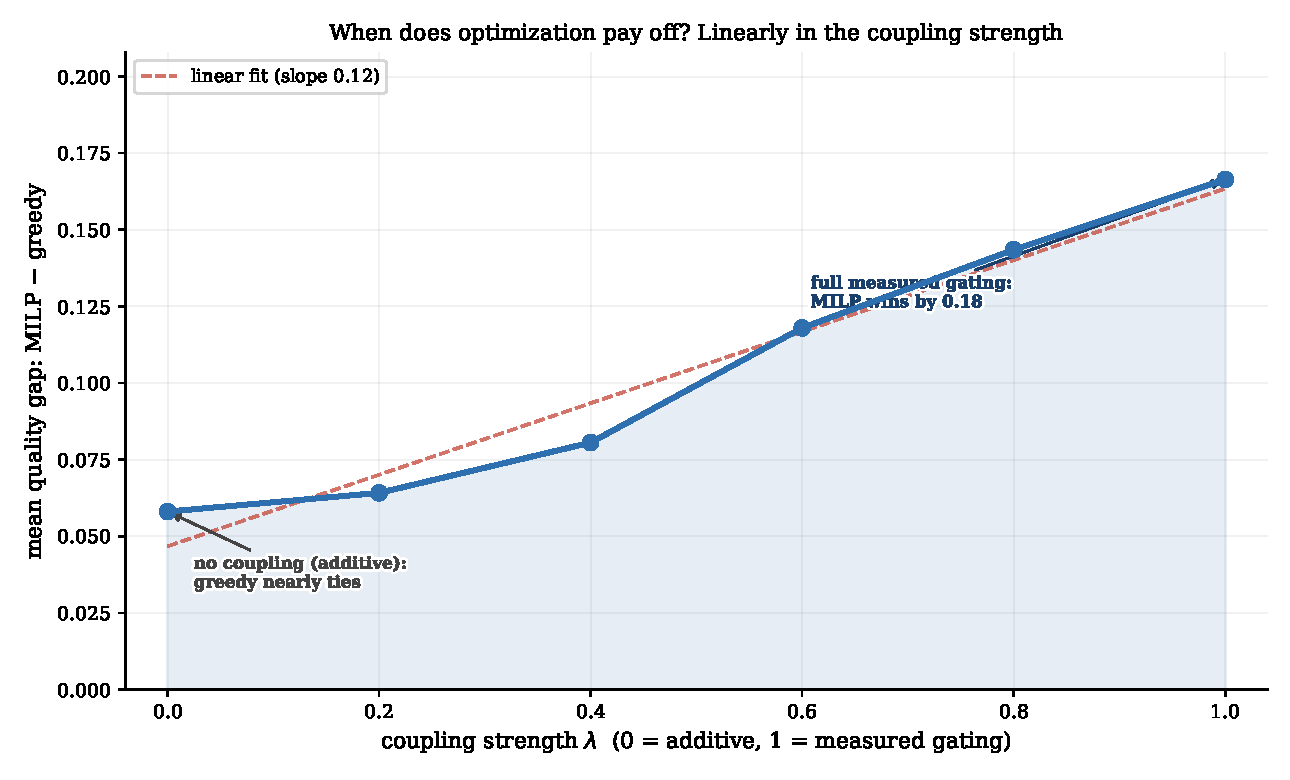
\includegraphics[width=0.9\textwidth]{fig/q17_coupling_sweep.pdf}
\caption{When optimization pays off. Mean quality gap between the gated MILP and a
greedy per-role heuristic, as a function of coupling strength $\lambda$
(\eqref{eq:lambda}; $0$ = additive, $1$ = full measured gating), $k{=}3$. The gap
grows near-linearly (slope $\approx0.11$): optimization is marginal when roles
decouple and increasingly valuable as gating tightens.}
\label{fig:coupling}
\end{figure}

\subsection{Robustness to execution mode: the batched extreme and an exact concurrent MILP}
\label{sec:batching}
Our primary latency model (§\ref{sec:milp}) treats the activated specialists as
running \emph{serially} on the shared GPU, $L_{\mathrm{sys}}=L_d+k\,L_s+L_y$---the
conservative worst case, since several specialists sharing one loaded model cannot
run truly in parallel on one instance. The opposite extreme is full \emph{batching},
in which the activated specialists are issued as a single forward pass and the stage
cost is one generation, $L_d+L_s+L_y$, independent of $k$. A real runtime sits
between these two. We treat the serial model as primary (it is the conservative
accounting, consistent with load-once memory, and the basis of the frontiers above)
and use this section to confirm the conclusions survive the batched extreme; the
exact batched model is what the released solver's \texttt{worst\_case} mode optimizes.

We introduce a \emph{serialization factor} $\sigma\in[\tfrac{1}{k},1]$ that
interpolates the specialist latency term,
\begin{equation}
L_{\mathrm{sys}}(k,\sigma)=L_d+\big(1+\sigma\,(k-1)\big)\,L_s+L_y,
\label{eq:sigma}
\end{equation}
so $\sigma{=}1$ is the serial model used as primary and $\sigma{=}\tfrac{1}{k}$
is ideal batching (the $k$ homogeneous specialists cost as much as one call).
$\sigma$ enters \emph{only} the latency constraint; the load-once memory bound and
all quality terms are unchanged, since a shared specialist occupies its memory once
regardless of execution mode. We re-solve the quality-aware MILP at $k{=}3$ across
the $\eps$-grid for $\sigma\in\{1,\,0.66,\,0.5,\,\tfrac{1}{3}\}$
(Fig.~\ref{fig:batching}).

\textbf{Result.} Batching shifts the frontier \emph{left}---the same quality at
lower latency---but does not change its shape or the optimal allocation. The
\emph{structural} optimum is invariant: the dispatcher and synthesiser remain large
and the specialist remains small (Llama-3.2-1B) in $100\%$ of budgets for
$\sigma\in\{1,0.66\}$, in $96\%$ at $\sigma{=}0.5$ (a single large-specialist
pick at the grid extreme $\eps{=}30$\,s), and in $84\%$ even at ideal batching
$\sigma{=}\tfrac{1}{3}$.
Crucially, across the realistic on-device regime $\eps\le20$\,s the specialist is
small at \textbf{$100\%$ of budgets in all four execution modes}. The choice
changes only at large budgets ($\eps\ge27$\,s) under strong batching
($\sigma\le0.5$), where a large specialist (Mistral-7B) becomes affordable---which is exactly the
expected behaviour: when batching makes the specialist term cheap and the budget is
generous, the optimizer can spend it on a large specialist without violating the
constraint. This does not weaken the three-regime finding; it confirms its
mechanism (the specialist is small \emph{because} of the latency cost of repeated
calls, and relaxing that cost is precisely what would admit a larger one).

\textbf{An exact concurrent MILP (the $\sigma{=}\tfrac1k$ endpoint, without
interpolation).} The serialization sweep \emph{estimates} batching by scaling the
latency term; we can instead model the batched endpoint \emph{exactly} inside the
program. Since the activated specialists share one loaded configuration, a single
batched pass costs the latency of that one configuration. Introduce a continuous
auxiliary $\Lambda\ge0$ and a cover constraint, replacing the sequential chain by
\begin{align}
L_{\mathrm{sys}}^{\mathrm{conc}} &= L_d + \Lambda + L_y \;\le\; \eps,
\label{eq:conc}\\
\Lambda &\ge \ell^{g}_{c}\,x_{s,c} \qquad \forall\,c .
\label{eq:conc-cover}
\end{align}
Because exactly one $x_{s,c}{=}1$, $\Lambda$ collapses to the chosen specialist's
generation latency, so $L^{\mathrm{conc}}_{\mathrm{sys}}=L_d+L_s+L_y$: this is the
$\sigma{=}\tfrac1k$ endpoint of~\eqref{eq:sigma}, expressed as one linear constraint
rather than a parametric scan. The linearization is exact (one auxiliary plus
$|\mathcal{K}_s|$ rows) and the program stays a sub-second MILP. (Both~\eqref{eq:sigma}
and~\eqref{eq:conc} use the single-stream performance table, so each is a
\emph{formulation} of batching rather than a measured batched-throughput campaign;
the two agree, and a direct measurement is left to future work.)

\textbf{Comparison.} Re-solving the full ten-model quality-aware MILP under the
sequential chain versus the exact concurrent chain (Fig.~\ref{fig:seqconc}) makes
the $\sigma{=}\tfrac1k$ endpoint exact rather than interpolated; it is the same
endpoint as the sweep, not an independent confirmation, but expressing it as a hard
constraint lets us read the feasibility boundary directly. Concurrent serving strictly enlarges the feasible
region: the pipeline becomes feasible from $\eps{=}4$\,s (versus $7$\,s
sequentially) and attains higher quality at every matched budget where both are
feasible. The \emph{allocation}, however, is invariant: the optimal specialist is
a sub-$1.3$\,B model at $100\%$ of feasible budgets under both chains: it is the
small Llama-3.2-1B everywhere ($13/14$ concurrent, $9/11$ sequential) except the
very tightest budgets ($\eps{=}4$\,s concurrent; $\eps{\le}8$\,s sequential), where
only the even smaller SmolLM2-360M fits the slot. The dispatcher and synthesiser grow with the
budget identically, and both frontiers plateau at the same $Q\approx1.60$. The
estimate and the exact formulation thus agree---the execution model moves the
frontier but leaves the three-regime optimum untouched.

\begin{figure}[H]
\centering

\includegraphics[width=\textwidth]{fig/fig_seq_vs_conc.pdf}
\caption{Quality--latency frontier under the sequential chain
($L_d+k\,L_s+L_y$) versus the exact concurrent chain
(Eqs.~\ref{eq:conc}--\ref{eq:conc-cover}), full pool, $k{=}3$. Concurrent serving
shifts the frontier left (feasible from $4$\,s versus $7$\,s, higher $Q$ at matched
$\eps$) but the optimal allocation---small Llama-3.2-1B specialist, large
dispatcher and synthesiser---is unchanged across the entire feasible range,
matching the $\sigma$-sweep of Fig.~\ref{fig:batching}.}
\label{fig:seqconc}
\end{figure}

\begin{figure}[H]
\centering
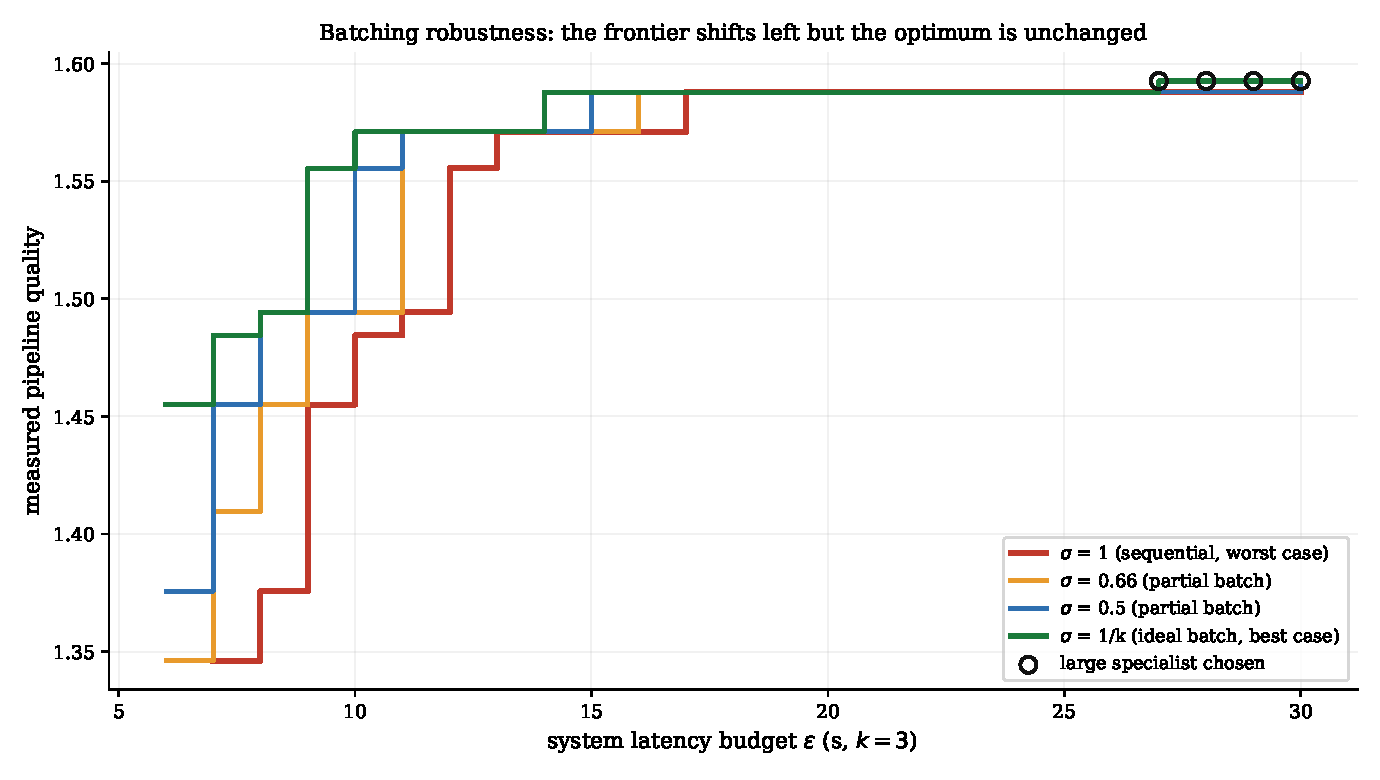
\includegraphics[width=\textwidth]{fig/q18_batching_robustness.pdf}
\caption{Robustness to execution mode ($k{=}3$). Quality--latency frontier under
the serialization factor $\sigma$~\eqref{eq:sigma}: $\sigma{=}1$ (sequential, worst
case) to $\sigma{=}1/k$ (ideal batching, best case). Batching shifts the frontier
left (lower latency for the same quality) but the small-specialist optimum is
unchanged across the realistic budget range.}
\label{fig:batching}
\end{figure}

\section{Generality of the Allocation Results}
\label{sec:generality}
This section answers \textbf{Q4}: which of the paper's modelling choices are
load-bearing? We isolate the two most consequential---the heterogeneous model pool
and the execution model---and test each as a controlled, single-variable change
against the same quality-aware MILP (§\ref{sec:qmilp}), the same memory budget
$M{=}6.99$\,GB, and the same measured quality tables. The execution-model half is
treated in §\ref{sec:batching} (the optimum is invariant under the exact concurrent
MILP); here we test the pool, and find that \emph{two} distinct findings of the
paper---the non-monotone three-regime structure (§\ref{sec:quality}) and the value
of modelling router--specialist coupling (§\ref{sec:bilinear})---both depend on it.
The picture that emerges is clean: what is load-bearing for the paper's quality
conclusions is the diversity of the candidate pool, not the latency accounting---the
two pool-dependent findings collapse in unison within a single dense family, while
the execution model leaves the optimum untouched.

\subsection{Single-family ablation: heterogeneity creates the three regimes}
\label{sec:family-ablation}
\textbf{Setup.} We restrict the pool from ten heterogeneous models to a single
dense family---Qwen2.5 in three sizes ($0.5/1.5/3$\,B), three quantizations, and
three contexts, i.e.\ $3\times3\times3=27$ configurations ($18$ of which satisfy the
specialist's minimum context $c_{\min}\ge4096$; all fit $M$). Every configuration carries the same measured quality used in
§\ref{sec:quality}, so the only changed variable is the \emph{diversity} of the
pool. The objective and the load-once memory accounting are identical to
§\ref{sec:qmilp}; the sweep is solved under the exact concurrent chain of
§\ref{sec:batching} with the agents' minimum-context constraints enforced---the
same execution model as the allocator of §\ref{sec:dyn-lean}---so the
single-family and full-pool analyses are compared like-for-like on the realistic
execution mode.

\textbf{No single family reproduces the full-pool optimum.} The headline finding
(§\ref{sec:quality}) is that specialist quality is \emph{non-monotone} in size and
peaks at Llama-3.2-1B (mean quality $0.754$), beating Mistral-7B ($0.736$) at
$6\times$ fewer parameters (pooled per-record means, the convention of the
§\ref{sec:quality} confidence intervals; the per-configuration scorecard means,
$0.74$/$0.72$, rank the models identically). That structure is a property of \emph{cross-family
heterogeneity}, and it is not reproduced inside any single family
(Fig.~\ref{fig:famquality}). The three families with more than one size behave
inconsistently and \emph{none} of them recovers the full-pool picture: within
Qwen2.5 quality is monotone \emph{increasing}
($0.493\rightarrow0.679\rightarrow0.716$ for $0.5\rightarrow1.5\rightarrow3$\,B),
whereas within both SmolLM2 ($0.659\rightarrow0.603$ for $0.36\rightarrow1.7$\,B)
and Llama-3.2 ($0.754\rightarrow0.712$ for $1.2\rightarrow3.2$\,B) it is monotone
\emph{decreasing}. The model that creates the full-pool peak---Llama-3.2-1B---wins
not because small is better within its own family in some universal sense, but
because the small member of \emph{one} family beats the large members of \emph{all}
others: the effect lives in the spread \emph{across} families at a fixed size, not
in a within-family law. A practitioner who restricts the pool to a single dense
family therefore sees an idiosyncratic, family-specific size--quality relation
(rising for Qwen, falling for SmolLM2 and Llama) and never the non-monotone
three-regime structure that justifies role-aware allocation.

\begin{figure}[H]
\centering

\includegraphics[width=\textwidth]{fig/fig_family_quality.pdf}
\caption{Measured specialist quality versus model size. Across all ten models
(grey) the relation is non-monotone and peaks at Llama-3.2-1B (circled, $1.2$\,B),
exceeding Mistral-7B at a fraction of the size. The three families with more than
one size disagree on the within-family trend---Qwen2.5 rises with size, while
SmolLM2 and Llama-3.2 fall---and none reproduces the full-pool non-monotonicity. The
effect is a cross-family one: the small member of one family (Llama-3.2-1B) beats
the large members of all others.}
\label{fig:famquality}
\end{figure}

\textbf{The small specialist becomes a constraint artifact.} Solving the
quality-aware MILP on the Qwen pool, the optimal specialist is the small $1.5$\,B
model at tight latency budgets---but for a reason unrelated to quality. Sweeping
$\eps$ (Fig.~\ref{fig:famsweep}), the specialist is $1.5$\,B for $\eps<11$\,s and
then \emph{switches to the largest $3$\,B model at $\eps{=}11$\,s}, the moment
the budget admits it. The $1.5$\,B choice is driven entirely by the latency of the
specialist on the critical path together with the load-once memory budget---sharing
the $1.5$\,B group between specialist and synthesiser frees memory for a large
dispatcher---and it disappears as soon as the budget relaxes. This is the opposite
of the full-pool behaviour, where Llama-3.2-1B is the optimal specialist at
\emph{every} budget (Table~\ref{tab:poolcontrast}) because it is the genuine
quality maximiser. In the full pool the small specialist wins \emph{on quality}; in
the single family it appears only \emph{under a tight constraint}.

\begin{figure}[H]
\centering

\includegraphics[width=\textwidth]{fig/fig_family_sweep.pdf}
\caption{Single-family (Qwen2.5) quality--latency frontier under the quality-aware
MILP ($k{=}3$). The optimal specialist is the small $1.5$\,B model only while the
budget is tight; it switches to the largest ($3$\,B) model at $\eps{=}11$\,s.
The small specialist here is a constraint artifact, not the quality-driven choice
that Llama-3.2-1B represents in the full pool.}
\label{fig:famsweep}
\end{figure}

\begin{table}[H]
\centering
\caption{Quality-aware optimum, full pool versus single family ($k{=}3$). In the
full pool the small specialist (Llama-3.2-1B) is optimal at \emph{every} budget on
quality from $\eps{=}5$\,s (at the single tightest budget only SmolLM2-360M fits the
slot, §\ref{sec:batching}); in the Qwen pool the small specialist is budget-bound and yields to the
largest model once $\eps$ grows. Dispatcher and synthesiser are large in both
regimes (§\ref{sec:qmilp}).}
\label{tab:poolcontrast}
\begin{tabular}{rll}
\toprule
$\eps$ (s) & pool & optimal specialist \\
\midrule
$\ge5$ & full (10 models) & Llama-3.2-1B (quality-optimal) \\
$<11$    & Qwen (1 family)  & Qwen2.5-1.5B (budget-bound) \\
$\ge 11$    & Qwen (1 family)  & \textbf{Qwen2.5-3B} (largest) \\
\bottomrule
\end{tabular}
\end{table}

\textbf{What the ablation establishes.} The role-aware allocation \emph{machinery}
is general---it runs unchanged on either pool, and the
large-dispatcher/large-synthesiser preference persists in both. But the paper's
sharpest empirical claim, that specialists prefer small models on quality, is a
consequence of having a \emph{diverse} pool that contains a small model genuinely
strong at grounded generation. A practitioner who restricts to one family will not
observe the three-regime effect and will, under a tight budget, reach a small
specialist for the wrong reason. This bounds the external validity of the finding
and reinforces its mechanism: heterogeneity is the source of the non-monotonicity,
and the optimizer is valuable precisely because it exploits cross-family structure
a single-family sort cannot see.

\subsection{The coupling result is also cross-family}
\label{sec:coupling-family}
The single-family ablation tests the \emph{capability} finding (§\ref{sec:quality});
we now apply the same controlled restriction to the \emph{coupling} finding
(§\ref{sec:bilinear}), to check whether the value of modelling router--specialist
gating is itself an artifact of pool diversity. We re-solve the gated bilinear MILP
and its coupling-blind additive counterpart on the Qwen-only pool, scoring both
under the true gating~\eqref{eq:gated}.

The result mirrors the capability case exactly. In the full pool the gated optimum
selects a \emph{different} dispatcher from the additive one at essentially every
budget---the small, high-recall SmolLM2-360M instead of the high-global-F1 Phi-3.5
or Mistral-7B---and dominates it by up to $0.32$ gated-quality points. Restricted to
Qwen2.5, that gap vanishes: the gated and additive optima select the
\emph{identical} dispatcher and specialist at every feasible budget ($33/33$
integer budgets, $\eps=8$--$40$\,s, under the sequential chain of §\ref{sec:bilinear};
$37/37$ under the concurrent chain), and the
gated-quality gap is zero. The reason is visible in the recall data: within Qwen the
model with the best global F1 (Qwen2.5-3B, $0.43$) is \emph{also} the model with the
best recall on the activated domains ($0.89$), so the global-F1 proxy and the
activated-domain recall agree and the coupling has nothing to exploit. In the full
pool they disagree sharply---SmolLM2-360M has the lowest global F1 ($0.39$) but
near-perfect activated-domain recall---which is exactly the gap the bilinear term
captures.

\textbf{A unified message.} Both of the paper's quality findings draw their force
from the same source. The non-monotone three-regime structure
(§\ref{sec:family-ablation}) and the value of modelling router--specialist coupling
(this section) are \emph{both} cross-family phenomena: each collapses in a
homogeneous pool and re-appears only when the candidate set spans families with
genuinely different size--quality and routing profiles. The execution model, by
contrast, leaves the optimum untouched (§\ref{sec:batching}). What is load-bearing
for this paper's conclusions is therefore the \emph{diversity of the candidate
pool}, not the latency accounting---and that diversity is the realistic default for
on-device multi-model deployment, where the whole point is to mix small specialised
models with a larger router and synthesiser.

\textbf{Scope of the two collapses.} The two results rest on different amounts of
evidence, and we state which. The capability collapse is visible across \emph{all
three} multi-size families (Qwen2.5, SmolLM2, Llama-3.2; Fig.~\ref{fig:famquality}),
none of which reproduces the full-pool non-monotonicity. The coupling collapse, by
contrast, is demonstrated on the \emph{single} family (Qwen2.5) that has both enough
sizes and enough per-domain routing instances to support the gated bilinear MILP;
the other two multi-size families are too small on the routing side to re-fit the
coupling cleanly. We therefore report the coupling collapse as a single-family
result---indicative of the same cross-family mechanism, but not a multi-family law.

\section{Dynamic Per-Query Allocation}
\label{sec:dynamic}
This section answers Q5. Every allocation so far is \emph{static}: the model in
each role is fixed before any query arrives, and each query pays for the same set
of activated specialists. Yet most queries need only a subset of the nine
specialists---a custody question needs \texttt{tutela\_minori}, not the succession
or matrimonial-property domains. Activating all of them wastes compute, and
activating the \emph{wrong} ones wastes compute and injects distractor context into
the synthesiser. We therefore add a \emph{dynamic} layer on top of the static
allocation that decides, per query, which specialist domains to run---making the
activation count $k(q)$ endogenous---while changing nothing about which model serves
each role. The static allocator (§\ref{sec:qmilp}--\ref{sec:bilinear}) chooses the
substrate; the dynamic layer routes over it.

\paragraph{Evaluation data and its provenance.}
\label{sec:dyn-data}
The static-allocation results of §\ref{sec:quality}--\ref{sec:bilinear} use the
$25$ gold-annotated queries of §\ref{sec:setting}, whose gold supporting-authority
\emph{passages} are required by the oracle-retrieval quality protocol. The dynamic
gate needs a different kind of supervision---gold \emph{routing} labels (which
specialists each query should activate), not gold passages---so for it we use an
expanded routing-annotated set, disjoint in purpose from the quality campaign and
described here for transparency. Three sources, mutually disjoint, are used and must
not be conflated: (i) the original $25$ gold-\emph{passage} queries supply the
per-domain corpus \emph{profiles} (the relevance signal is similarity to these gold
passage texts); (ii) a larger set of $94$ routing-annotated queries (\texttt{expected\_agents}
labels only, no gold passages) is used solely to \emph{calibrate} the gate's
thresholds; and (iii) a held-out \emph{test} set of $64$ queries ($49$ in-domain
across the nine domains, $15$ deliberately out-of-scope) is used only to
\emph{evaluate}. The $94$-query calibration set and the $64$-query test set have
zero identifier overlap (verified), and neither overlaps the $25$-query
profile set; so threshold-fitting, profiling, and testing are performed on disjoint
data and the evaluation involves no leakage. We stress that the in-domain metric
below is \emph{routing} accuracy against gold \texttt{expected\_agents}, a proxy for
answer quality, not reference-checked answer correctness; §\ref{sec:limits} states
this bound precisely.

\subsection{An LLM-free per-query gate}
\label{sec:dyn-gate}
For a query $q$ a candidate set $C(q)$ of specialist domains is proposed---by the
deployed dispatcher, or, in the variant studied here, by a retrieval router---and a
calibrated gate prunes $C(q)$ to the selected set $S(q)\subseteq C(q)$, so
$k(q)=|S(q)|$. The gate uses one signal: the similarity between $q$ and each
domain's corpus profile, profiles built offline from the $25$-query gold passage
texts (§\ref{sec:dyn-data}), embedded with the same \texttt{bge-m3} encoder used
throughout. Crucially the gate loads \emph{no} second language model---it is a
calibrated function of an embedding similarity---so it adds nothing to the load-once
memory budget $M$ that governs the static allocation, and it is therefore free in
exactly the resource the rest of the paper optimizes.

Let $\rho_d(q)\in[0,1]$ be the calibrated relevance of domain $d$ to $q$, obtained
by isotonic regression of the raw fused similarity onto gold relevance labels.
Domain $d$ is admitted to $S(q)$ when $\rho_d(q)\ge\tau_d$. The per-domain
thresholds $\{\tau_d\}$ are \emph{learned from the $94$-query calibration set}, not
hand-set, by maximizing a recall-favoring $F_\beta$ criterion of the kept set
against the gold specialist set,
\begin{equation}
\tau_d \;=\; \arg\max_{\tau}\; F_\beta\!\big(\{\rho_d(q)\ge\tau\},\,\mathrm{gold}_d\big),
\qquad \beta\ge 1,
\label{eq:fbeta}
\end{equation}
subject to three robustness controls that matter in the small-calibration regime:
a \emph{recall floor} forbidding any $\tau$ that drops more than a fixed fraction of
a domain's calibration positives (this rules out the degenerate ``threshold so high
that nothing passes'' solution); a hard ceiling $\tau\le\bar\tau$; and
empirical-Bayes \emph{shrinkage} of each per-domain $\tau_d$ toward the global
threshold with weight proportional to the domain's sample count, so thin-sample
domains borrow strength from the pool. We take $\beta=3$ (recall-favoring), the
appropriate bias for a legal assistant where dropping a relevant specialist is
costlier than running an extra one. When no candidate clears its threshold,
$S(q)=\varnothing$ and the pipeline abstains---the desired response to an
out-of-scope query.

\subsection{Routing and latency results}
\label{sec:dyn-results}
We report routing precision, recall, and $F_1$ against the gold specialist set, and
latency from the measured performance table (Eq.~\ref{eq:derive}) via the selected
$k(q)$---the same axis as the static frontiers of §\ref{sec:opt} and
§\ref{sec:qmilp}.

\paragraph{Main result.}
Table~\ref{tab:dyn-main} and Fig.~\ref{fig:dyn-main} compare static-$k$ routing
(the candidate set run in full) against dynamic gating at $\beta=3$, across three
static allocations: the quality-aware optimum (§\ref{sec:qmilp}), the gated optimum
(§\ref{sec:bilinear}), and a single-family Qwen allocation. Static routing has high
recall ($0.93$) but low precision ($0.24$): the router proposes about six of nine
domains and most are wrong. The gate roughly doubles precision (to $0.43$) while
conceding seven points of recall (to $0.86$), raising $F_1$ from $0.33$ to $0.50$
($+0.17$) and cutting mean activation from $6.0$ to $3.61$. The routing metrics are
\emph{identical} across the three allocations---the gate is allocation-independent,
and the allocations separate only on latency (qwen $9.69$\,s $<$ gated $10.76$\,s
$<$ qa $11.07$\,s). The routing gain therefore transfers across allocations while
cost does not. (We note that this $F_1$ baseline of $0.33$ is the candidate set
proposed by the LLM-free retrieval router and is a distinct quantity from the
per-model dispatcher routing $F_1$ of §\ref{sec:quality}, which reaches $0.68$; the
two are not directly comparable, as the former scores a multi-domain candidate set
and the latter a single model's full routing decision.)

\begin{table}[H]
\centering
\caption{Static-$k$ versus dynamic routing on the $64$-query held-out test set
($\beta=3$, per-domain $F_\beta$ thresholds, \texttt{bge-m3}). Latency from the
measured performance table under the concurrent model. Routing metrics are identical
across allocations (the gate is allocation-independent); the allocations differ only
in latency.}
\label{tab:dyn-main}
\small
\begin{tabular}{llccccc}
\toprule
allocation & routing & $F_1$ & prec. & rec. & $k$ & lat.\,(s)\\
\midrule
qa-optimum    & static  & 0.33 & 0.24 & 0.93 & 6.00 & 12.18\\
              & dynamic & \textbf{0.50} & 0.43 & 0.86 & 3.61 & 11.07\\
gated-optimum & static  & 0.33 & 0.24 & 0.93 & 6.00 & 11.87\\
              & dynamic & \textbf{0.50} & 0.43 & 0.86 & 3.61 & 10.76\\
qwen          & static  & 0.33 & 0.24 & 0.93 & 6.00 & 10.67\\
              & dynamic & \textbf{0.50} & 0.43 & 0.86 & 3.61 & \phantom{0}9.69\\
\bottomrule
\end{tabular}
\end{table}

\begin{figure}[H]
\centering
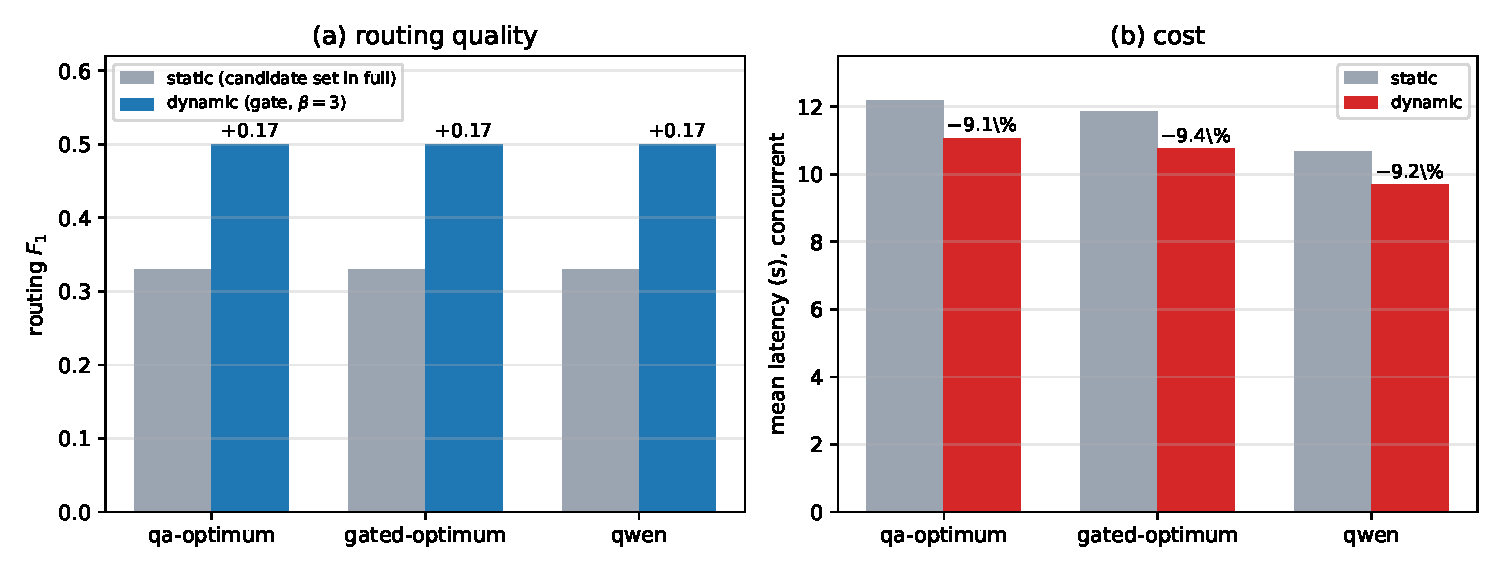
\includegraphics[width=\textwidth]{fig/dyn_routing_main.pdf}
\caption{Dynamic routing improves $F_1$ by $0.17$ at every allocation (a) while
cutting latency by $\approx9\%$ under the concurrent model (b). The routing gain is
allocation-independent; only latency differs across allocations.}
\label{fig:dyn-main}
\end{figure}

\paragraph{The precision--recall knob and the latency model.}
Sweeping the $F_\beta$ parameter (Fig.~\ref{fig:dyn-beta}) traces the operating
curve. As $\beta$ rises from $1$ to $5$, recall climbs from $0.80$ to $0.86$ and
mean $k$ from $3.12$ to $3.61$, with $F_1$ nearly flat ($0.49$--$0.50$); $\beta=3$
is the knee ($\beta=5$ changes nothing). The latency reduction depends on the execution model exactly as the
static analysis of §\ref{sec:batching} predicts. Under the concurrent model---where
specialists sharing a loaded model run in one batched pass, so the specialist stage
costs a single call---the reduction is pinned at $9.1$--$9.3\%$ regardless of $k$, because
latency then depends on \emph{whether} specialists run, not how many. Under the
sequential model the reduction is $27$--$35\%$ and grows with the pruning. We report
the concurrent figure as the conservative headline and the sequential figure as the
serial-execution case, consistent with the dual treatment in §\ref{sec:batching}.

\begin{figure}[H]
\centering
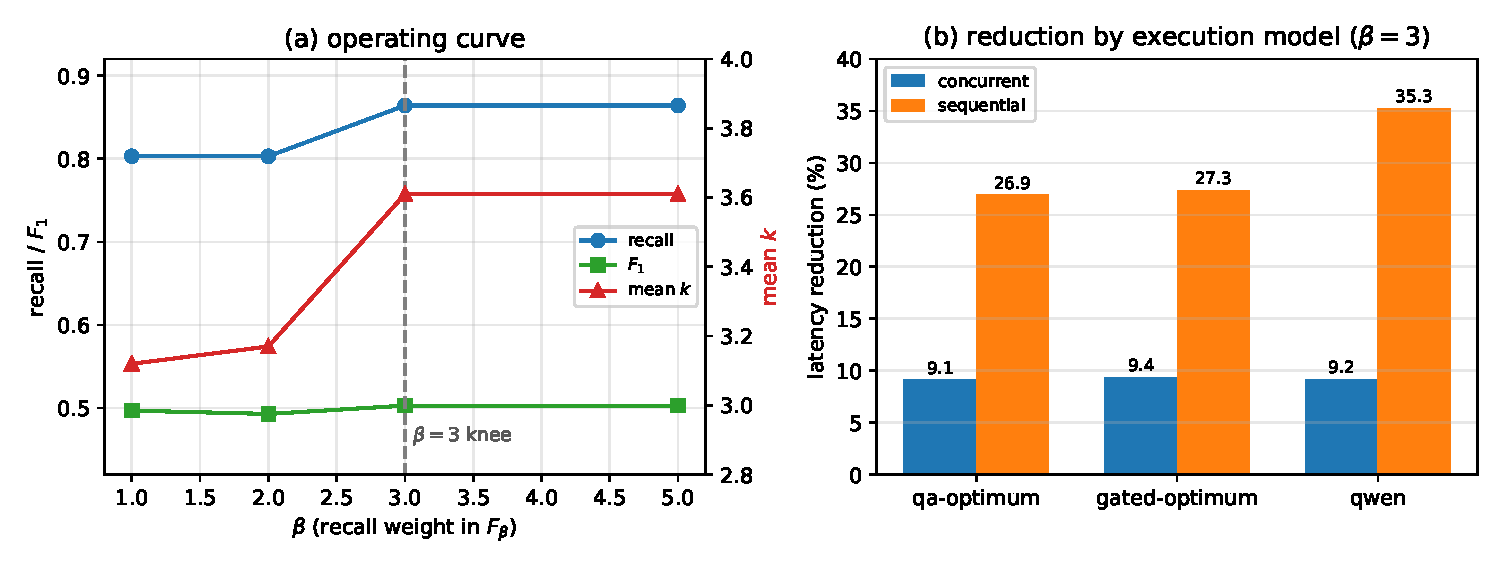
\includegraphics[width=\textwidth]{fig/dyn_beta_sweep.pdf}
\caption{(a) Quality versus the $F_\beta$ objective: recall and $k$ rise with
$\beta$, $F_1$ is flat, $\beta=3$ is the knee. (b) Latency reduction is $\approx9\%$
under concurrent serving (insensitive to $k$) and $27$--$35\%$ under sequential
serving (sensitive to $k$)---the same execution-model dichotomy as §\ref{sec:batching}.}
\label{fig:dyn-beta}
\end{figure}

\paragraph{Calibration scale is the dominant factor.}
Table~\ref{tab:dyn-calib} and Fig.~\ref{fig:dyn-calib} isolate the effect of
calibration size, and it echoes the small-$n$ caveat that runs through
§\ref{sec:quality}. With only $25$ routing-annotated queries over nine domains
($2$--$3$ positives each), the per-domain $F_\beta$ fit overfits and produces
degenerate thresholds up to $0.467$; the gate becomes precision-obsessed ($0.92$
precision, $0.39$ recall, $k=0.6$), abstaining on almost everything, at $F_1=0.37$.
Scaling to the $94$-query calibration set ($7$--$29$ positives per domain) lifts
$F_1$ to $0.50$, restores recall to $0.86$, and caps the maximum threshold at
$0.166$. The robustness controls of §\ref{sec:dyn-gate} are the safety net for the
thin-sample regime; with enough calibration they become largely non-binding---sweeping
the recall floor over $\{0.7,0.8,0.9,1.0\}$ leaves $F_1$ within $[0.48,0.50]$, so the
operating point is governed by the data and the objective, not by a finely-tuned
threshold.

\begin{table}[H]
\centering
\caption{Calibration-scale ablation ($\beta=3$, evaluated on the same $64$-query
test set). A larger calibration set removes the degenerate thresholds of the
small-sample regime and rebalances the gate from near-total abstention to a
productive precision/recall trade.}
\label{tab:dyn-calib}
\small
\begin{tabular}{lccccc}
\toprule
calibration & $F_1$ & prec. & rec. & $k$ & $\max\tau$\\
\midrule
$25$-query & 0.37 & 0.92 & 0.39 & 0.62 & 0.467\\
$94$-query & \textbf{0.50} & 0.43 & 0.86 & 3.61 & 0.166\\
\bottomrule
\end{tabular}
\end{table}

\begin{figure}[H]
\centering
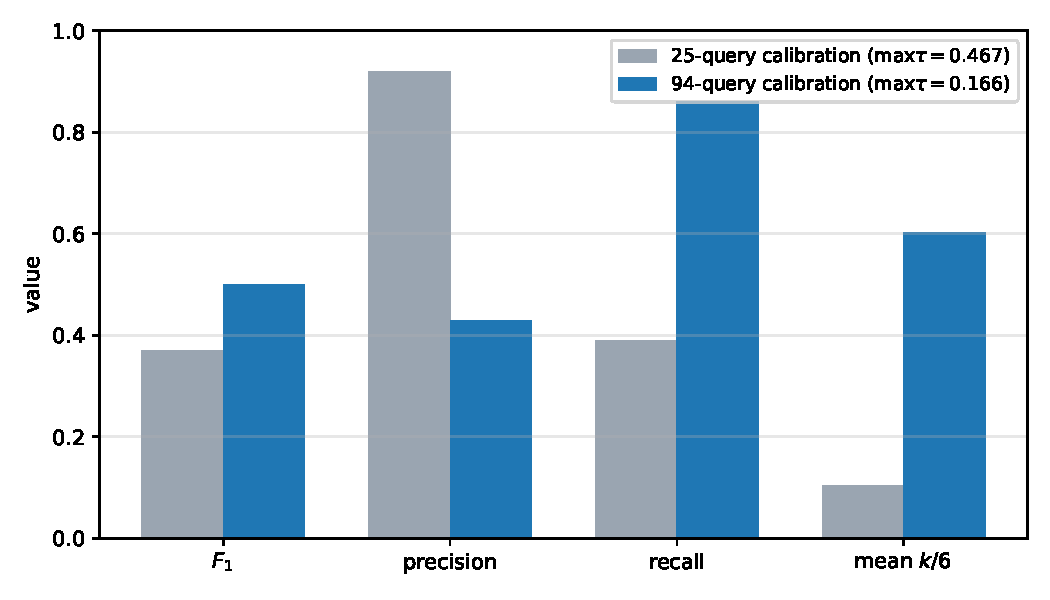
\includegraphics[width=0.74\textwidth]{fig/dyn_calib_ablation.pdf}
\caption{Scaling calibration from $25$ to $94$ queries raises routing $F_1$ from
$0.37$ to $0.50$ and eliminates the degenerate, over-abstaining thresholds of the
small-sample regime (mean $k$ shown divided by $6$).}
\label{fig:dyn-calib}
\end{figure}

\subsection{Out-of-distribution behaviour}
\label{sec:dyn-ood}
A legal assistant must decline questions outside its competence. On the $15$
out-of-scope queries of the test set the LLM-free gate abstains on $0.60$ ($9/15$),
with mean false activation $0.80$. The structure of the failures is the finding
(Fig.~\ref{fig:dyn-ood}): every leak is a succession- or family-adjacent query that
is \emph{on-topic but out-of-scope}---foreign-jurisdiction questions (Brazilian
succession, German custody, Spanish property) and malformed inputs (a bare keyword,
a wrong-language query, lorem-ipsum noise)---each routed into the topically-nearest
Italian domain. A purely semantic gate cannot separate ``Italian succession'' from
``Brazilian succession,'' which are near-identical in embedding space: \emph{the
gate captures topic but not jurisdiction.} Detecting jurisdiction would require an
explicit signal (a language or country classifier, or jurisdiction-tagged corpora),
which we leave to future work. Under the deployed LLM dispatcher (rather than the
LLM-free retrieval router evaluated here) abstention is substantially higher; the
two configurations answer different questions and we report them separately rather
than interchangeably.

\begin{figure}[H]
\centering
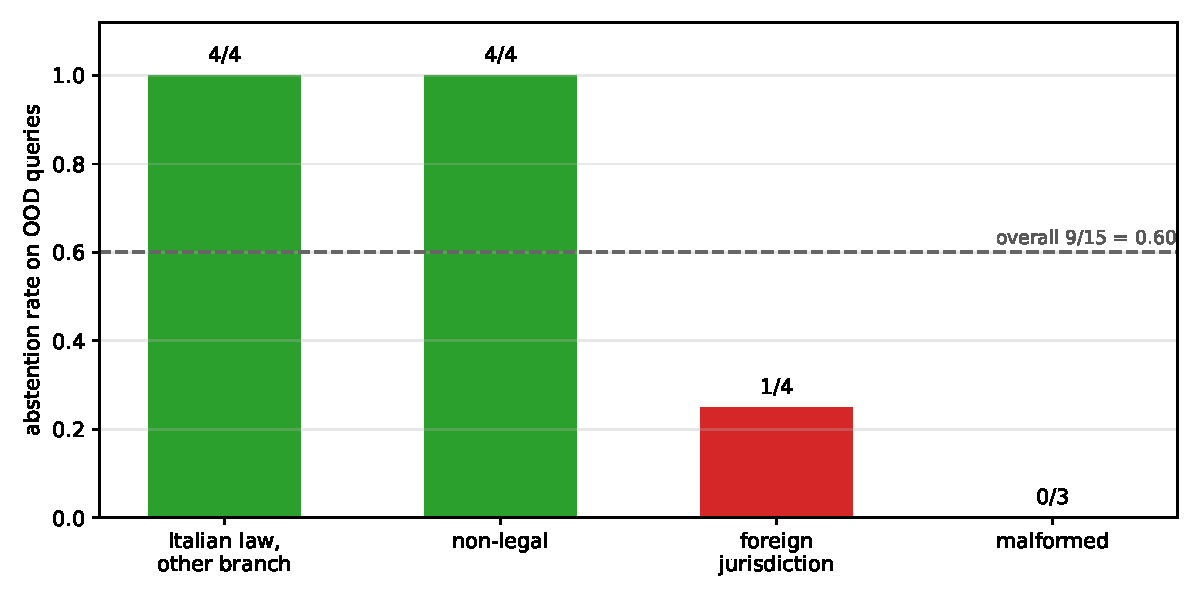
\includegraphics[width=0.86\textwidth]{fig/dyn_ood.pdf}
\caption{OOD abstention. The gate abstains on every topically-unrelated query and
leaks only on topic-near, scope-far inputs (foreign jurisdiction, malformed),
isolating a semantic-gating limitation rather than a calibration failure.}
\label{fig:dyn-ood}
\end{figure}

\subsection{A single-objective concurrent-batch allocator}
\label{sec:dyn-lean}
The dynamic layer is orthogonal to the static allocation; we close by strengthening
the static model itself for the concurrent regime that §\ref{sec:batching}
identified as the realistic on-device execution mode. We pose a compact
single-objective allocator that maximizes pipeline quality
$Q = F_d + \frac{1}{|D|}\sum_{\delta} Q_{s,\delta} + Q_y$ under a hard memory budget
and a hard latency SLA $T^\circ$, using the exact concurrent latency of
§\ref{sec:batching},
\begin{equation}
L_{\text{total}} \;=\; L_d(c_d) + \Lambda + L_y(c_y), \qquad
\Lambda \;\ge\; \ell^g_{c}\,x_{s,c}\ \ \forall c,
\label{eq:dyn-conc}
\end{equation}
where the single auxiliary $\Lambda$ collapses to the chosen specialist's latency
(exactly one $x_{s,c}=1$), so a batched specialist stage costs one call. Solved with
HiGHS on the measured Qwen instance at $M=6.99$\,GB and $T^\circ=8$\,s, it selects a
\texttt{Qwen2.5-3B} (Q8) dispatcher and a \emph{single shared} \texttt{Qwen2.5-1.5B}
(Q5) group serving both specialist and synthesiser, at $Q=1.88$, $L=8.00$\,s (the SLA
binds), $5.43$\,GB: only two weight groups are loaded, and it is precisely the
load-once sharing of the 1.5B group that frees the memory for the 8-bit 3B
dispatcher. It beats the naive baselines (largest-fits $1.39$, uniform $1.60$); the
per-role-best baseline reaches a higher nominal
$Q=1.95$ but is \emph{infeasible}, breaching the SLA at $11.0$\,s while fitting in
memory---the joint memory--latency coupling the MILP respects and the heuristic
ignores. The sequential-versus-concurrent comparison
(Fig.~\ref{fig:dyn-lean}) restates, in this single-objective setting, the result of
§\ref{sec:batching}: concurrent serving attains $Q\ge$ sequential at \emph{every}
SLA and remains feasible at tight SLAs ($T^\circ=4$--$6$\,s) where the sequential
model admits no feasible allocation. Concurrent batching both enlarges the feasible
region and dominates on quality, independently confirming the execution-mode
robustness reported for the full pool in §\ref{sec:batching}.

\begin{figure}[H]
\centering
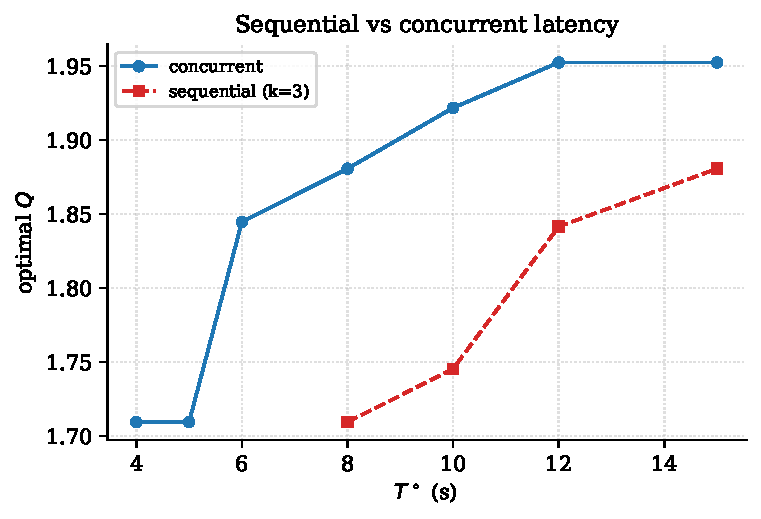
\includegraphics[width=0.78\textwidth]{fig/dyn_lean_concurrent.pdf}
\caption{Single-objective concurrent-batch allocator: concurrent
($L_d+\Lambda+L_y$) versus sequential ($L_d+kL_s+L_y$) serving on the measured Qwen
instance. Concurrent serving attains higher quality at every SLA and is feasible in
the shaded region where sequential serving is not, matching the full-pool finding of
§\ref{sec:batching}.}
\label{fig:dyn-lean}
\end{figure}

\subsection{What the dynamic layer establishes}
Holding a measured static allocation fixed, a calibrated LLM-free gate that selects
specialists per query improves routing $F_1$ by $0.17$ and reduces latency by
$10$--$33\%$ (concurrent vs.\ sequential), with a gain independent of the underlying
allocation and an operating point set by calibration data rather than hand tuning.
The improvement is purchased at no additional memory---the binding resource of the
whole paper---because the gate is a function of an embedding similarity, not a second
model. Two honest bounds carry into §\ref{sec:limits}: the in-domain metric is
routing accuracy, not reference-checked answer correctness, and the LLM-free gate's
OOD abstention is limited by its inability to detect jurisdiction. The complementary
single-objective concurrent allocator reproduces, in a compact form, the
execution-mode result of §\ref{sec:batching}: batched serving Pareto-dominates
sequential serving in quality and feasibility.


\section{Discussion and Limitations}
\label{sec:limits}
\textbf{What the optimization establishes---and what it does not.} The objective
is distinct-model parameter count, a transparent \emph{capability proxy}, not
measured answer quality. The frontier states \emph{how much distinct model} the
pipeline can afford at each latency, not \emph{how good} its answers are. The
answer-quality measurement (judge-free embedding-based scoring of routing,
grounding, and synthesis) is still running, and we fabricate no quality numbers.
The same MILP accepts a quality objective directly---replace $\pi_m$
in~\eqref{eq:obj} with measured per-role quality and gate the specialist term by
routing accuracy---so the present result is a coherent performance-space
allocation and a validated scaffold for the quality-aware version. Because the
measured-quality campaign (§\ref{sec:quality}) shows capability does not track
parameter count, we expect the quality-optimal frontier to differ from
Fig.~\ref{fig:frontier}, and do not present the latter as a quality result.

\textbf{An honest assessment of the optimization's value.} On the
performance-only proxy a greedy sort matches the MILP on $92\%$ of the frontier
(§\ref{sec:opt}): for that sortable objective we do not claim the optimization is
necessary. Its value appears when the objective stops being sortable. We
demonstrate this with heterogeneous specialists---distinct legal domains with
per-domain model affinities---where the MILP beats greedy on $92\%$ of points and
on \emph{all} points once enough specialists are active, because the best joint
assignment trades model quality across domains under shared budgets in a way a
per-slot sort cannot. That demonstration uses \emph{synthetic} affinities and is
labelled as such; its role is to locate the regime where optimization is
required. The production objective---measured per-domain answer quality---lives
in exactly that non-sortable regime, which is why the MILP, not a heuristic, is
the right tool once the quality table exists.

\textbf{Other limitations.} (1) The serial-sum
latency~\eqref{eq:chain-intuition} assumes the activated specialists share one
loaded instance and run one after another (the conservative worst case); if they are
instead batched into a single forward pass the stage cost falls to one generation,
which we model exactly in §\ref{sec:batching} and find the optimum unchanged. True
latency on a given runtime lies between these two extremes. (2) All
measurements are from a single device under one driver; absolute numbers shift on
other hardware, though the qualitative curves should transfer and the perf table
is cheap to re-measure. (3) Derived latency~\eqref{eq:derive} assumes throughput
independent of output length, mildly optimistic for long outputs. (4) Peak VRAM
via NVML may under-report transient spikes. (5) The activation count $k$ is
treated as a parameter, not modelled from the query distribution; the $k{=}3$
curve approximates the dataset mean of $2.68$. (6) The quality evaluation rests on
$37$ root queries and is under-powered per domain ($7$ of $9$ domains have
$n<10$); we report bootstrap CIs and rely on pooled and cross-role signals rather
than individual small-$n$ per-domain claims. A leave-one-domain-out check
(§\ref{sec:quality-heldout}) indicates the specialist selection is not in-sample
overfitting---the train-selected model is Llama-3.2-1B in all nine folds with a
$0.001$ mean held-out generalization gap---but with only $37$ root queries the
quality-aware frontier is still best read as an in-sample optimum whose absolute
values are optimistic, even though the \emph{selection} generalizes. (7) The primary
quality-aware objective~\eqref{eq:qobj} is additive; we relax this with a measured
bilinear router--specialist gating (§\ref{sec:bilinear}), but that estimate uses
the same small per-domain samples, so its specific dispatcher winner is indicative
rather than definitive. (8) RAGAS embedding-based scores are taken
as the quality ground truth and not validated against human legal judgement; the
synthesiser aggregate in particular reduces largely to correctness. (9) The
batching analysis (§\ref{sec:batching}) \emph{parametrizes} the sequential$\to$batched
range via the serialization factor $\sigma$; the performance table is measured
single-stream, so we do not claim a specific measured batching speedup---we show
only that the optimal allocation is invariant across the whole $\sigma$ range.
Measuring batched throughput directly is left for future work. (10) The
non-monotone three-regime finding and the value of modelling router--specialist
coupling are both established on a heterogeneous pool; §\ref{sec:generality} shows
each collapses within a single dense family (where, depending on the family, the
size--quality relation is monotone in either direction, and the gated and additive
optima coincide). The external validity of both results is therefore bounded to
multi-family catalogues---which are the realistic deployment setting, but the
single-family case should not be expected to exhibit them. (11) The dynamic-layer
evaluation (§\ref{sec:dynamic}) scores \emph{routing} accuracy against gold
\texttt{expected\_agents}---a proxy for, not a measurement of, answer correctness;
we have no reference answers for the $64$-query test set, so the dynamic layer's
in-domain numbers establish that it activates the right specialists, not that the
resulting answers are better, though removing distractor specialists makes a quality
loss unlikely. (12) The LLM-free gate's out-of-distribution abstention ($0.60$) is
bounded by its inability to detect \emph{jurisdiction}: it captures topic but routes
foreign-jurisdiction queries into the topically-nearest Italian domain
(§\ref{sec:dyn-ood}). The higher abstention obtainable with the deployed LLM
dispatcher is a different configuration and is not interchangeable with the
LLM-free figure; we report them separately.

\section{Conclusion}
We characterized the performance of $75$ quantized SLM configurations on a single
$8$\,GB GPU---throughput, memory, latency, energy, their precision/context/scale
cost curves---and
we posed and solved an explicit MILP that allocates models to the pipeline's
three generation roles to maximize distinct-model capacity under a load-once
memory budget and a serial system-latency budget, parametric in the number of
activated specialists. We held the optimization to a strict standard: for the
sortable parameter objective a greedy heuristic matches it on $92\%$ of points,
which we report rather than hide. The optimization becomes necessary, not
marginal, once the objective is not sortable---demonstrated (on synthetic
per-domain affinities) by heterogeneous specialists, where the MILP wins on $92\%$
of points and on all points when enough specialists are active. Finally, the
measured-quality campaign across all three roles reveals three distinct scaling
laws: routing (dispatcher) and synthesis quality rise with model size, while
domain-grounded specialist quality is non-monotone and peaks at a $1.2$\,B
model---so the roles prefer opposite ends of the size spectrum, the capacity
proxy is sub-optimal in quality at every latency budget, and per-role allocation
is empirically justified. Acting on this, the quality-aware MILP---the same
program with measured quality replacing the proxy---traces the measured
quality--latency frontier, independently recovers the mixed three-regime optimum
(large dispatcher, small specialist, large synthesiser), beats fixed-model
policies, and dominates the parameter-proxy allocator at every matched-latency
budget by a mean of $0.13$ quality points. Modelling the router--specialist
coupling as a bilinear term---exactly linearized and solved on measured data---goes
further: the gated optimum dominates the coupling-blind additive optimum at $42$ of
$44$ budgets and reveals that the right router is the one with high recall \emph{on
the activated domains}, not high global F1. We give a mechanistic account of the
three regimes---a role's optimal model size tracks its grounding requirement, so
classification-like roles (routing) reward scale while context-faithful roles
(grounded specialists) penalize it---turning the empirical finding into a testable
prediction. And we characterize \emph{when} optimization is worth it: the
MILP-over-greedy gap grows near-linearly with how strongly the pipeline gates
downstream agents on upstream decisions, from $0.06$ (decoupled) to $0.18$ (full
measured gating). Finally, a generality analysis isolates what the conclusion
depends on: both the non-monotone specialist regime and the value of modelling
router--specialist coupling are cross-family phenomena that collapse within a single
dense family, whereas the small-specialist optimum is robust to the
serial-versus-batched execution model---so the result is driven by pool
diversity rather than by the execution accounting. The central lesson is that a
parameter proxy and a measured-quality objective induce materially different
optimal configurations, and that role couplings matter: in a multi-agent pipeline,
allocation must be driven by measured, coupling-aware per-role quality, which a
single global heuristic cannot replace. Finally, the allocated substrate can itself
be made query-adaptive at no memory cost: a calibrated, LLM-free per-query gate that
selects which specialists to activate raises routing $F_1$ from $0.33$ to $0.50$ and
cuts latency $10$--$33\%$ with a gain independent of the underlying allocation, and a
single-objective concurrent-batch MILP confirms batched serving Pareto-dominates
sequential serving in quality and feasibility---so static allocation, coupling-aware
optimization, and per-query adaptation compose into one coherent on-device design.
All data, the MILP, the baselines, and the
plotting code are released.

\vspace{6pt}
\hrule
\vspace{4pt}
{\small\textbf{Reproducibility.} The performance table ($75$ configurations), the
MILP (\texttt{syscap\_milp.py}, PuLP/CBC), the frontier data
(\texttt{syscap\_frontier.csv}), and all plotting scripts are released. Latency
and energy are derived via Eq.~\eqref{eq:derive} at $T=384$ tokens. Capacity is
parameter count, an explicit capability proxy, not measured quality. The headline
capacity--latency frontiers (Fig.~\ref{fig:frontier}, Table~\ref{tab:frontier}) use
the serial chain of Eq.~\eqref{eq:chain-intuition} and are reproduced by the released
solver with \texttt{--latency-model sequential --k-activated} $k$ for
$k\in\{1,3,5,9\}$; the exact batched model of §\ref{sec:batching} is the solver's
\texttt{worst\_case} mode, and the interpolating $\sigma$-sweep is also released. The
dynamic-layer experiments of §\ref{sec:dynamic} are likewise released: the
per-query routing/latency evaluation (\texttt{routing\_eval.py}), the
out-of-distribution abstention test (\texttt{ood\_eval.py}), the end-to-end pipeline
runner (\texttt{run\_pipeline.py}), and the single-objective concurrent-batch
allocator (HiGHS), together with the three disjoint query sets used---the $25$-query
gold-passage profiles, the $94$-query routing-annotated calibration set, and the
$64$-query held-out test set (§\ref{sec:dyn-data}). The gate's thresholds are fit by
the per-domain $F_\beta$ procedure of Eq.~\eqref{eq:fbeta} with $\beta=3$. The §\ref{sec:dynamic}
routing/abstention numbers use \texttt{bge-m3} relevance scores; the released
package replays them offline once the one-time score cache
(\texttt{build\_score\_cache --embedder bge-m3}) is committed, and a
dependency-free hashing embedder validates the pipeline end-to-end without it.}

\begin{thebibliography}{99}
\small
\bibitem{cascadia} Y.~Jiang, F.~Fu, W.~Zhao, S.~Rabanser, N.~D.~Lane, and B.~Yuan,
``Cascadia: An Efficient Cascade Serving System for Large Language Models,''
\emph{arXiv:2506.04203}, 2025.
\bibitem{cascadetrain} (Cascade-Aware Training of Language Models),
\emph{arXiv:2406.00060}, 2024.
\bibitem{semanticcascade} ``Semantic Agreement Enables Efficient Open-Ended LLM
Cascades,'' \emph{arXiv:2509.21837}, 2025.
\bibitem{cascaderouting} J.~Dekoninck, M.~Baader, and M.~Vechev, ``A Unified
Approach to Routing and Cascading for LLMs,'' \emph{ICML}, 2025 (arXiv:2410.10347).
\bibitem{routingsurvey} ``Dynamic Model Routing and Cascading for Efficient LLM
Inference: A Survey,'' \emph{arXiv:2603.04445}, 2026.
\bibitem{routellm} I.~Ong, A.~Almahairi, V.~Wu, W.-L.~Chiang, T.~Wu,
J.~E.~Gonzalez, M.~W.~Kadous, and I.~Stoica, ``RouteLLM: Learning to Route LLMs with
Preference Data,'' \emph{arXiv:2406.18665}, 2024.
\bibitem{moa} J.~Wang, J.~Wang, B.~Athiwaratkun, C.~Zhang, and J.~Zou,
``Mixture-of-Agents Enhances Large Language Model Capabilities,''
\emph{arXiv:2406.04692}, 2024.
\bibitem{masurvey} ``Multi-Agent Collaboration Mechanisms: A Survey of LLMs,''
\emph{arXiv:2501.06322}, 2025.
\bibitem{ragas} S.~Es, J.~James, L.~Espinosa-Anke, and S.~Schockaert, ``RAGAs:
Automated Evaluation of Retrieval Augmented Generation,'' \emph{EACL System
Demonstrations}, 2024 (arXiv:2309.15217).
\bibitem{slmquant} ``SLMQuant: Benchmarking Small Language Model Quantization for
Practical Deployment,'' \emph{arXiv:2511.13023}, 2025.
\bibitem{edgeslm} ``Edge Deployment of Small Language Models: A Survey,''
\emph{arXiv:2511.22334}, 2025.
\bibitem{ondevicellm} ``On-Device LLMs: State of the Union, 2026,'' technical
report, 2026.
\bibitem{quanteval} ``Which Quantization Should I Use? A Unified Evaluation of
\texttt{llama.cpp} Quantization on Llama-3.1-8B-Instruct,'' \emph{arXiv:2601.14277},
2026.
\end{thebibliography}

\end{document}
